% !TeX spellcheck = en_GB
\documentclass{article}
\usepackage{graphicx}
\usepackage{titlesec}
\usepackage{array}
\usepackage[table]{xcolor}
\usepackage{color, colortbl}
\usepackage{stackengine}
\usepackage{fancyhdr}
\usepackage{longtable}
\usepackage{changepage}
\usepackage{tikz, graphicx}
\usepackage{hyperref}
\usepackage{listings}
\usepackage{float}

\newcommand\xrowht[2][0]
{\addstackgap[.5\dimexpr#2\relax]{\vphantom{#1}}}

\setlength{\arrayrulewidth}{0.4mm}
\setlength{\tabcolsep}{20pt}
\renewcommand{\arraystretch}{1.6}
\setcounter{tocdepth}{4}
\setcounter{secnumdepth}{4}

\pagestyle{fancy}
\renewcommand{\headrulewidth}{2pt}
\renewcommand{\footrulewidth}{1pt}

\begin{document}
\begin{titlepage}
	\begin{center}
		\begin{figure}
			\centering
			
\includegraphics[scale=0.3]{LogoPolimi.PNG} \\
			[0.3cm]
		\end{figure}
		\Huge{\bfseries - DD -} \\
		[0.5cm]
		\huge{Design Document} \\
		[1mm]
		\rule{300pt}{3pt} \\
		[1.0cm]
		\textsc{\Large Computer Science and Engineering} \\ 
		\textsc{\Huge Software Engineering II} \\
		\textsc{\Large A.A. 2020/2021} \\
		[1cm]
		\textsc{\LARGE Daniele Mammone - 10625264} \\
		\textsc{\LARGE Gianmarco Naro - 10610374} \\
		\textsc{\LARGE Massimo Parisi - 10583470} \\
	\end{center}
\end{titlepage}

\newpage

\renewcommand\contentsname{Contents}
\tableofcontents

\newpage

\section{Introduction}

	\subsection{Purpose}
	The main target of this document is to describe the {\bfseries Customer Line-Up} (\emph{CLup}) design from a more detailed point of view. This document follows faithfully what was defined in the Requirement Analysis and Specification Document and must be read carefully before starting the software implementation in order to understand the software design in detail. Moreover, we tried to maintain independence between \emph{DD} document and \emph{RASD} document in order to allow greater flexibility in case you want to reuse the design model.
	
	\subsection{Scope}
	\emph{CLup} is a booking application and nowadays this type of applications are more and more widespread in people's everyday life and are becoming more and more indispensable. For this reason, intelligent design choices have been made that extrapolate the positive aspects of existing booking apps, in order to make CLup really “achievable” in real life.
	
	The main purpose of CLup is to facilitate customers to access at a store in {\bfseries security}, both allowing them to reserve a spot on the queue for entering the store through the app and to book a visit at the store at a determined time of a certain day, selected by the customer. Thanks to this, store managers can manage the {\bfseries affluence} in their store more easily, and moreover can reduce the crowd in front of the store, that is one of the main purposes of the application. Another important feature deals with obtaining statistics from customers and generic information from stores in order to help customers during their reservation. For this, the system has to store a very large amount of data. This data are mined and used later, which is why it is very important to identify the user's role so that we can provide him with more accurate and suitable information. Indeed a customer wants to provide information about the stores while, for example, a store manager is more interested in information about customer permanence in the store.
	
	\subsection{Definitions, Acronyms, Abbreviations}
	\bigskip
		\subsubsection{Definitions}
			\begin{center}
				\rowcolors{2}{}{gray!20}
				\rowcolors{1}{gray!20}{white}
				\renewcommand{\arraystretch}{2.5}
				
				\begin{adjustwidth}{-2.3cm}{}
					\begin{tabular}[h!]{|m{8em}|m{31em}|}
						\hline
						\xrowht{5pt}
						QR Code & Bi dimensional bar code that allows the user to check-in/check-out at the store entries/exits \\
						\xrowht{5pt}
						Reservation & Indicates both booked visits and spots on the queue to enter the store as soon as possible \\
						\xrowht{5pt}
						Customer & The clients of the store, that uses the system to get a reservation to access the store \\
						\xrowht{5pt}
						Store manager & The app user that access to stores’ bookings, occupancy and settings, in order to manage the flow of customers \\
						\xrowht{5pt}
						QR Code Reader & Device used to scan customers’ \emph{QR Code} \\
						\xrowht{5pt}
						Totem & Electronic device that allows customers to physically get a spot on the queue to enter the store a soon as possible; it allows to specify the same parameters that can be inserted through the app \\
						\xrowht{5pt}
						QR Code Printer & Device used by totems to print \emph{QR Code} \\
						\xrowht{5pt}
						Department & Part of the store that contains the same category of products \\
						\xrowht{5pt}
						Query & Synonym for request \\
						\hline
					\end{tabular}
				\end{adjustwidth}
			\end{center}
		\subsubsection{Acronyms}
			\begin{center}
				\rowcolors{2}{}{gray!20}
				\rowcolors{1}{gray!20}{white}
				\renewcommand{\arraystretch}{2.5}
				
				\begin{adjustwidth}{-2.3cm}{}
					\begin{tabular}[h!]{|m{4em}|m{35em}|}	
						\hline
						\xrowht{5pt}
						\centering RASD & Requirement Analysis and Specification Document \\
						\xrowht{5pt}
						\centering DD & Design Document \\
						\xrowht{5pt}
						\centering ETA & Estimated Time of Arrival \\
						\xrowht{5pt}
						\centering GPS & Global Positioning System \\
						\xrowht{5pt}
						\centering API & Application Programming Interface \\
						\xrowht{5pt}
						\centering UML & Unified Modeling Language \\
						\xrowht{5pt}
						\centering DBMS & DataBase Management Service \\
						\xrowht{5pt}
						\centering OS & Operative System \\
						\xrowht{5pt}
						\centering HTTPS & HyperText Transfer Protocol over Secure Socket Layer \\
						\xrowht{5pt}
						\centering TCP & Trasmissione Control Protocol \\
						\xrowht{5pt}
						\centering IP & Internet Protocol \\
						\hline	
					\end{tabular}
				\end{adjustwidth}
			\end{center}
		\bigskip
		\subsubsection{Abbreviations}
			\begin{center}
				\rowcolors{2}{}{gray!20}
				\rowcolors{1}{gray!20}{white}
				\renewcommand{\arraystretch}{2.5}
				
				\begin{adjustwidth}{-2.3cm}{}
					\begin{tabular}[h!]{|m{4em}|m{35em}|}
						\hline
						\xrowht{5pt}
						\centering IIT & Implementation, Integration and Testing \\
						\xrowht{5pt}
						\centering Rn & Requirement number n \\
						\xrowht{5pt}
						\centering ASAP & As soon as possible \\
						\xrowht{5pt}
						\centering POV & Point of view \\
						\hline
					\end{tabular}
				\end{adjustwidth}
			\end{center}
	\subsection{Revision History}
		\begin{center}
			
			\renewcommand{\arraystretch}{1.5}
			\begin{adjustwidth}{-2.3cm}{}
				\begin{tabular}[h!]{|m{4em}|m{5em}|m{26em}|}	
					\hline
					\rowcolor{gray!20}
					\xrowht{5pt}
					\centering Version & \centering Date & Changelog \\
					\hline
					\xrowht{5pt}
					\centering 1.0 & 24/12/2020 & First version \\
					\hline	
				\end{tabular}
			\end{adjustwidth}
			
		\end{center}
	\subsection{Software and Tools}
		\begin{itemize}
			\item {\LaTeX} as software system for docuement preparation
			\item UMLet for the UML diagrams and other diagrams
			\item Photoshop for the mockups
			\item Git \& Github as work space. The repository is \href{https://github.com/danmaam/MammoneNaroParisi}{here}.
		\end{itemize}
	\subsection{Reference Documents}
		\begin{itemize}
		\item Specification Document
		\item Slides of the lectures
		\end{itemize} 
	\subsection{Document Structure}
		The structure of the document is thought with the intention of allowing simple navigation through it. Also, various abbreviations, highlighted in Abbreviations section, have been used to make the content smoother.
		Hence, the structure of the document is the following one:
		\begin{itemize}
			\item {\bfseries Introduction}: this section gives a general view of the problem and describes the scope and purpose of the \emph{DD}, including a set of definitions, acronyms and abbreviations used.
			
			\item {\bfseries Architectural Design}: this section starts with a high level description of the architecture of the system and continues going into details, specifying the components and interfaces used.
			
			\item {\bfseries User Interface Design}: this section presents the mockups of the application, describing how the clients can navigate the application, highlighting the actions they can do.
			
			\item {\bfseries Requirements Traceability}: this section describes the connection between the RASD and the DD, identifying the relation between goals and requirements described previously and the components that allow to realize them.
			
			\item {\bfseries Implementation, Integration and Test Plan}: this section establishes a plan for the development of components, identifying the conditions needed to be met before starting the development process and then maximizing the efficiency of the developer teams with a precise schedule.
			
			\item {\bfseries Effort Spent}: the main focus of this section is to track the time spent to complete this project. In particular, is highlighted the subdivision of the working hours of the various sections.
			
			\item {\bfseries References}: this section is dedicated to all references used in this project.
		\end{itemize}

\section{Architectural Design}
	The aim of this section is to give a look to the architectural aspect of the analyzed system. In doing this, a top-down approach will be followed, starting from a very general view of the system, then going into more detail through {\bfseries Component Diagrams}, more and more detailed. This allows us to precisely describe each component of \emph{CLup}, so that who will develop the system, well know the behaviour of each component.
	
	\subsection{Overview}
	A first high level overview can be done through the system's \textbf{Composition Diagram}. In fact, here there is a first subdivision of the system's component, each one with a different task.
	\begin{itemize}
		\item \textbf{Communication Interfaces}: to work properly, the system needs to interface overt the network with both remote applications, and external services. Because of this, there are some components devoted to interact with remote devices:
		\begin{itemize}
			\item{\bfseries UserHandler}: to interact with users, both managers and customers, the latter both at \emph{totems}, and on app.
			\item{\bfseries EntranceManagement}: so that the store can process a scanned \emph{QR Code} at entry/exit.
			\item{\bfseries NumberCallingInterface}: to notify the call of a certain number.
		\end{itemize}
		and others deputy to access external services, such as 
		\begin{itemize}
			\item{\bfseries Map Component}: to access an external {\bfseries Map Provider}.
			\item{\bfseries Notification Component}: to send notifications to customers through an external {\bfseries Notification Service}.
			\item{\bfseries Mail Component}: to externally sending mails, avoiding building an internal {\bfseries Mail Manager}.
		\end{itemize}
	\begin{figure}[!h]
		\centering
		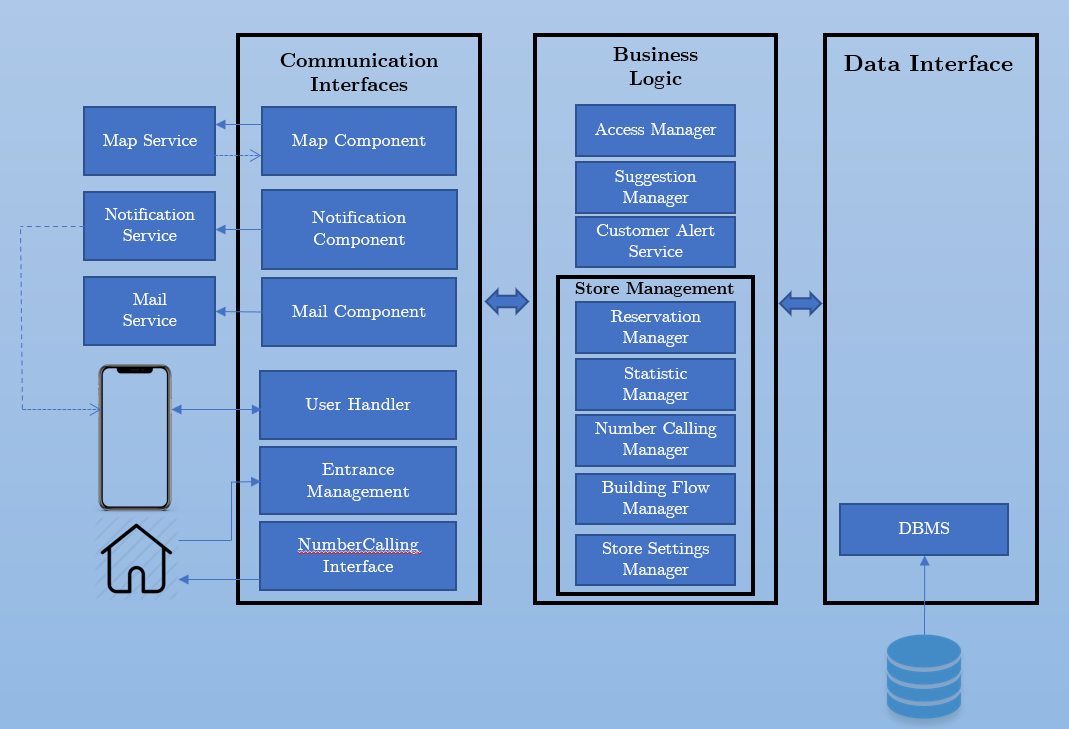
\includegraphics[scale=0.5]{../UML Diagrams/CompositionDiagram/CompositionDiagram.png} \\
		\caption{\emph{Number calling system}}
	\end{figure}
	
		\item{\bfseries Business Logic}: here there is the whole Business Logic of the system. Since each store may maintain a different logic from another, there is a Component for each store managed by the system. Each store, manages the following aspects:
		\begin{itemize}
			\item{\bfseries Reservation Manager}: manages all the things concerning reservations and their making. It's useful also to retrieve some important data, such as \emph{ETA}s and available time intervals to enter the store.
			\item{\bfseries Statistic Manager}: it's the part used for the calculation of statistics about customers' shopping time, and about the average time spent in a single department. Since each store is different from the other, the statistics are maintained unique per store. This part is also used by \textbf{Reservation Manager} to calculates \emph{ETA}s and time intervals;
			\item{\bfseries Number Calling System}: is the component dedicated to admit reserved customers inside the store.
			\item{\bfseries Building Flow Manager}: it takes care of processing scanned \emph{QR Codes} at the entry and the exit of the store.
			\item{\bfseries Store Settings Manager}: manages all the things concerning stores' settings and parameters, such as working hours and capacity (also for each department).
			
		\end{itemize} This subdivision allows to separate better the logic off each store. Moreover, there are component common to each store, so the ones deputy to allow users to request services to the system.
		\begin{itemize}
			\item {\bfseries Access Manager}: manages users' registraion and log-in;
			\item {\bfseries Suggestion Manager}: manages the retrieve of suggestions when required, or necessary;
			\item{\bfseries Customer Alert Service}: takes care of sending departing notifications to customers.
		\end{itemize}
	At the end, there is another block: the \textbf{Data Interface}: it represents the \emph{Data Tier} of the system and separates the Business Logic from the data. It interacts with the \emph{DBMS} to store and load informations.
	\end{itemize}

	
	\subsection{Component View}
		The aim of this section is to give a look to the architectural aspect of the analyzed system. In doing this, a top-down approach will be followed, starting from a very general view of the system, then going into more detail through {\bfseries Component Diagrams}, more and more detailed. This allows us to precisely describe each component of \emph{CLup}, so that who will develop the system, well know the behaviour of each component.\\
		
		\begin{itemize}
			\item {\bfseries MobileApp}: it is the component relative to the mobile application used by store managers and customers; in order to access \emph{CLup} services. It uses three interfaces: \emph{CustomerInterface}, \emph{StoreInterface}, used to access functionalities respectively for customers and store managers, and \emph{AccessInterface}, that allows users to log-in and register.
			
			\item {\bfseries CLupServer}:  it is the component deputy to manage users’ access, and customers requests.
			
			\item {\bfseries StoreComponent}: it is the component that principally manages the business logic of the system, since takes care of the functionalities associated with a single store. Each store will have its own {\bfseries Store Component} deployed in a dedicated container. The aim of this is to separate the critical functionalities of each store, to reduce the risk of a complete block of the system and to make maintenance easier in case of malfunctionalities of a single store.
			
			\item {\bfseries TotemApp}: it is the component that represents the interface used by a physical totem installed at stores in order to request the issue of a ticket. The totem interface is separated from the Mobile App’s one, since a totem can request tickets only to the store where it’s installed, directly communicating with it.
			
			\item {\bfseries ScannerApp}: it is the component that represents \emph{QR Scanners}’, that asks the associated store to process the scanned \emph{QR Codes}.
			
			\item {\bfseries NumberCallingApp}: it is the component deputy to notify at stores that a number has been called. It’s used by the associated store to notify that some customers are admitted to enter the store.		
		\end{itemize}
	
		Moreover, to exploit some features, \emph{CLup} relies on some external services, using them through their \emph{API}s:
		
		\begin{itemize}
			\item {\bfseries MapsAPI}: exploits the \emph{API}s of an external map services, necessary to compute percurrency times and sort stores depending on the position.
			
			\item {\bfseries NotificationAPI}: it is the interface used to send notifications to customers’ devices. Since each mobile \emph{OS} already has its own notification system, \emph{CLup} exploits this in sending notifications, without the need of building a new in-house notification service.
			
			\item {\bfseries EmailAPI}: it is the interface used to communicate with a mail provider service, to send emails to customers.
			
			\item {\bfseries DBMSAPI}: the interface used to access the Data Logic of \emph{CLup}.
		\end{itemize}
	
		It has been chosen to not develop these features, since there isn’t a real necessity of making them from scratch: the existing ones work well, are already tested and complete (for example, developing an internal map service will require inserting the whole world cartography, while a non \emph{OS}-integrated notification service must deal with aggressive \emph{OS}es’ power management). Moreover, this outsourcing allows to reduce the time for developing the system, and the maintenance costs, since it’s externally done by the service provider.

		\begin{figure}
			\begin{adjustwidth} {-3cm}{}
				\centering
				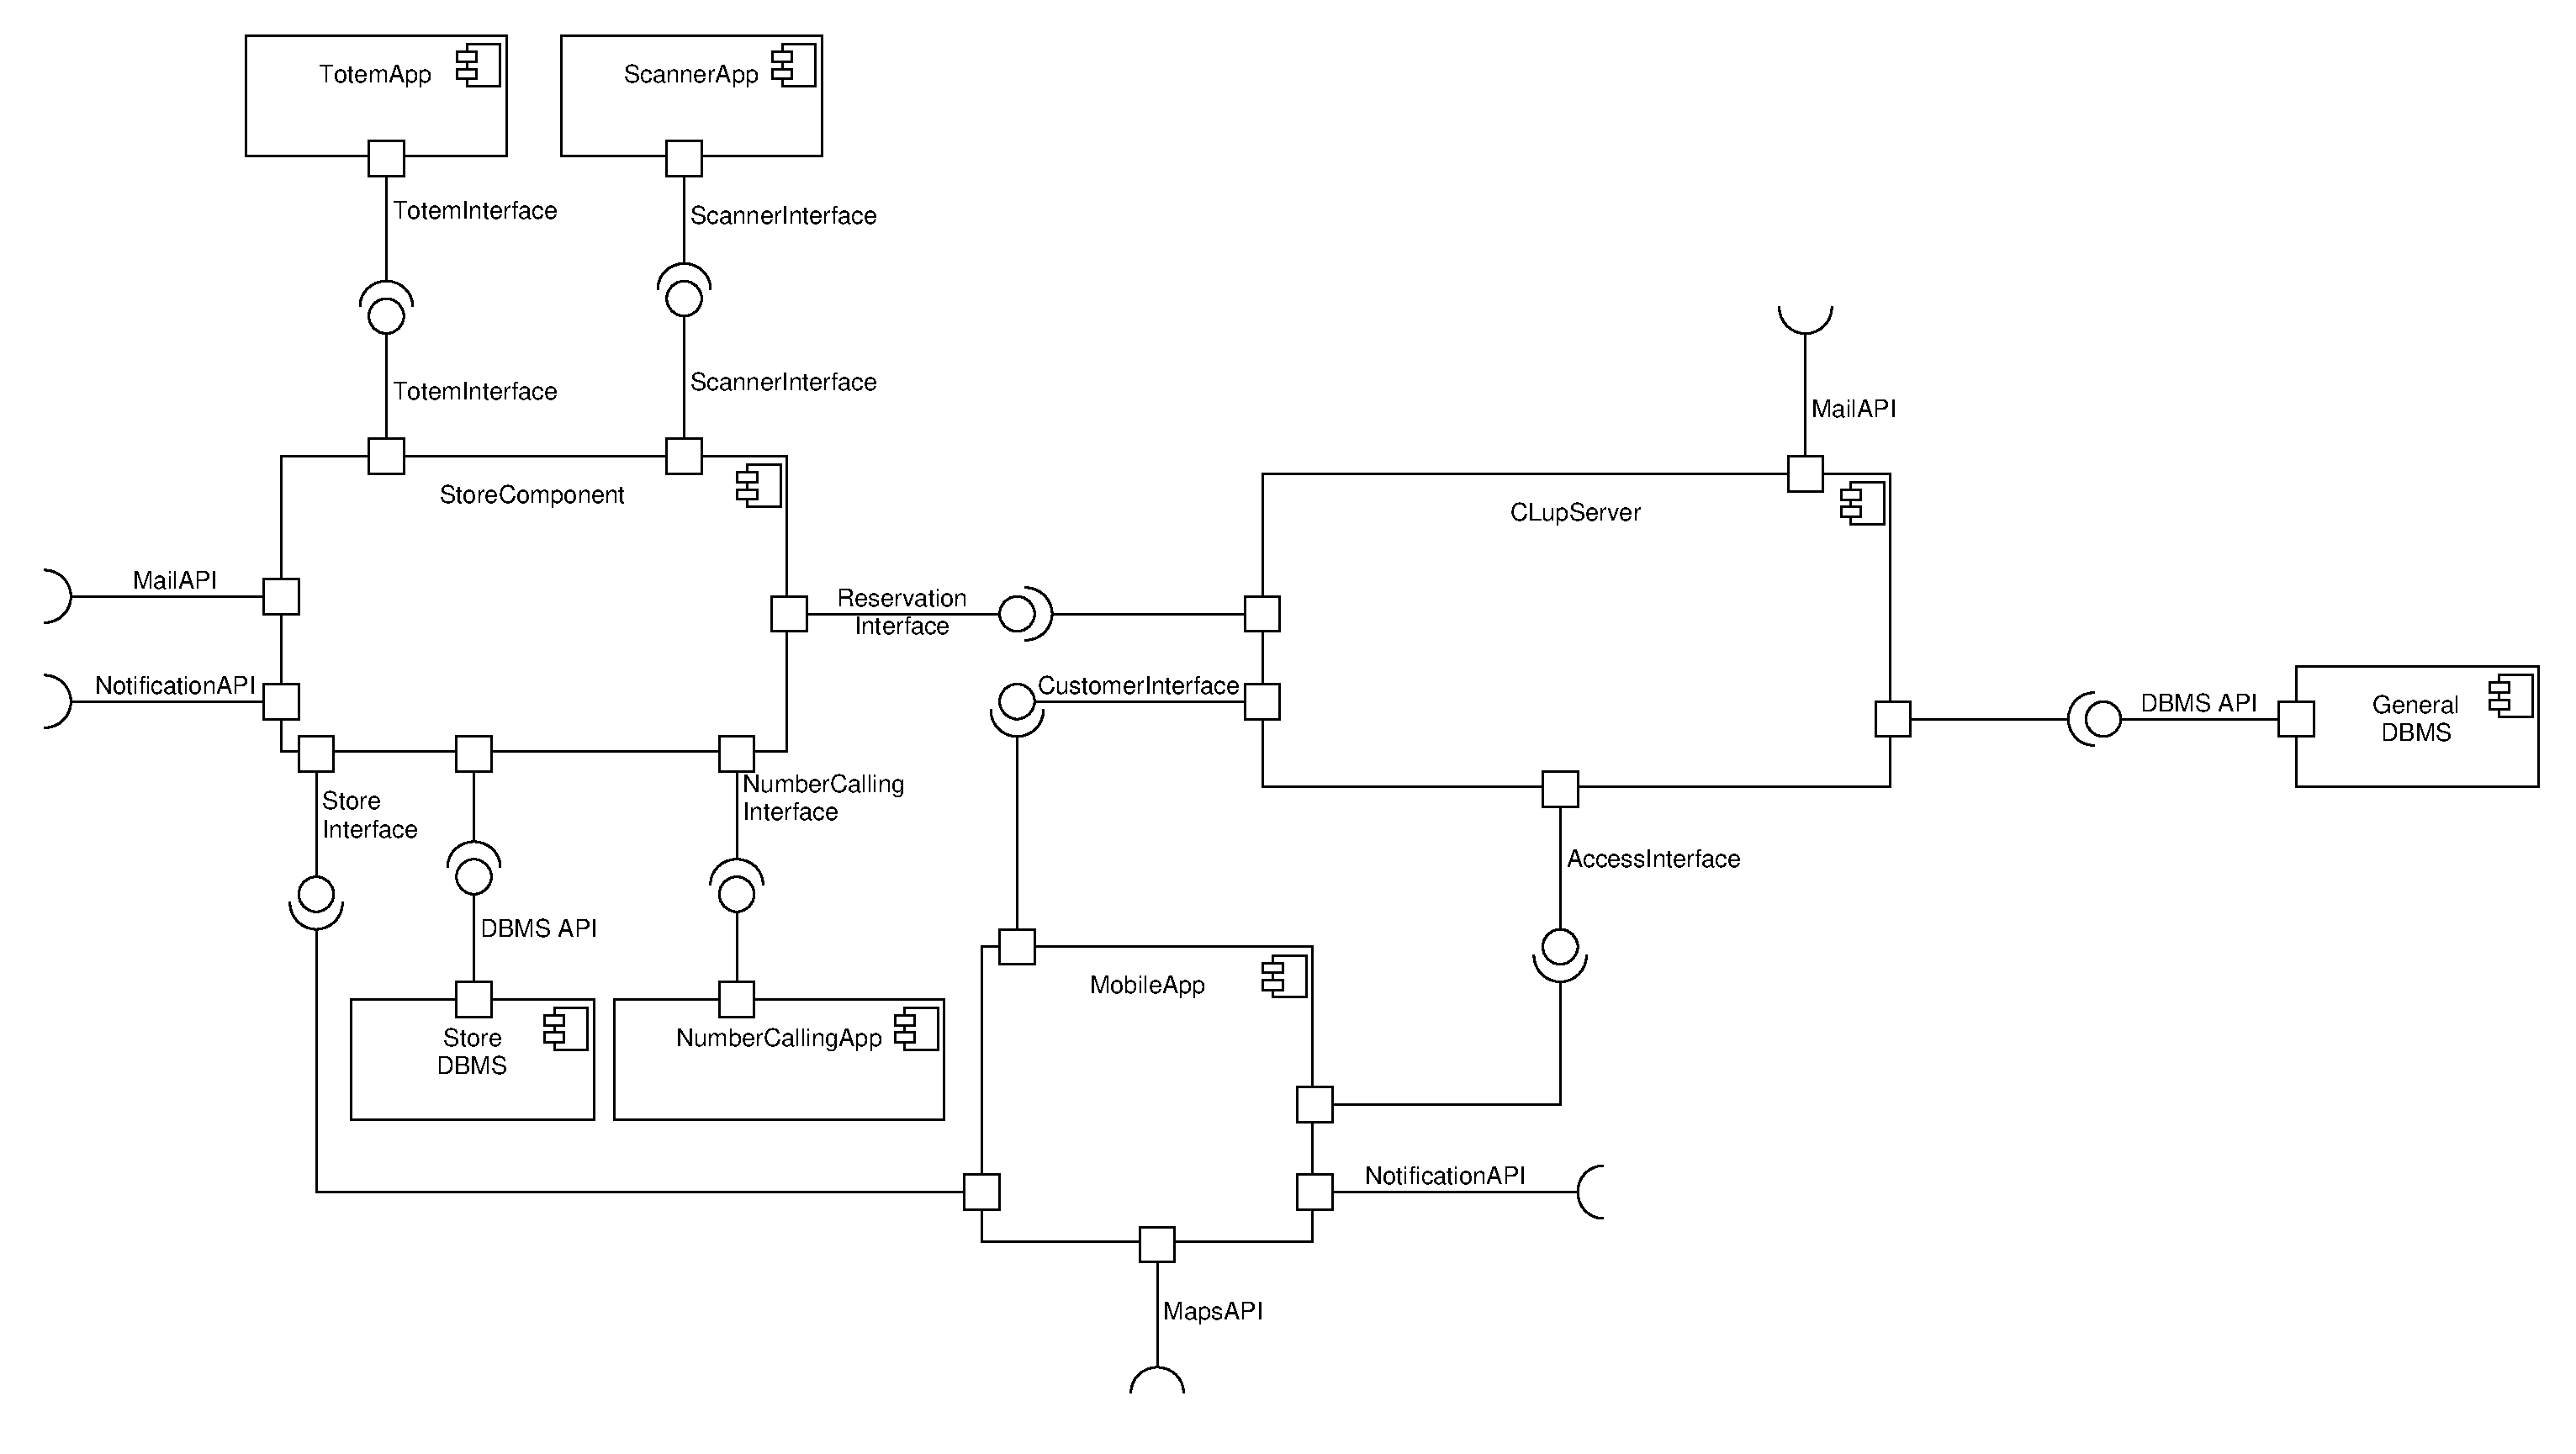
\includegraphics[scale=0.35, angle=90, trim= 0 0 0 -5cm]{Component Diagrams/HighLevelComponentDiagram.pdf}\\
			\end{adjustwidth}
			\caption{\emph{High Level Component Diagram}}
		\end{figure}
		\newpage
		\subsubsection{Adapters}
			The system uses some “Adapters” to access the external services; no \emph{API}s are directly exposed to any component but the adapters. So, it is sufficient to change the corresponding adapter to migrate to another service, without the need of rewriting code of other components. Moreover, if required in some circumstances, it’s possible to use different external services: it is sufficient to use the correct adapter in order to access the desidered service.
			
			\begin{itemize}
				\item {\bfseries MapManager}: it is the component that takes requests from other components, and redirect them to the chosen external {\bfseries Map Service}.
				
				\item {\bfseries NotificationComponent}: since each mobile \emph{OS} uses its own notification service, this adapter takes in requests of notification sending, and redirect them to the correct service; the latter will take care of delivering the notification to the customer.
				
				\item {\bfseries MailComponent}: an adapter used to send emails; as the previous ones, allows to change the used mail service painlessly.
				
				\item {\bfseries DataManager}: probably, the most important adapter of the system, since it is the one connecting the other components to the system’s data logic. 
			\end{itemize}
		
		Here, there is described the one for \emph{DBMS}, since it’s the most articulated among those.
		
			\paragraph{Data Manager Component}
				The Data Manager is the component that manages the requests for data manipulation. The components analyzed two aspects:
				
				\begin{itemize}
					\item Data Manipulation
					\item Query Execution
				\end{itemize}
			
				The components’ services are requested through the \emph{DataInterface}, while it access to the \emph{DBMS} through its \emph{API}s. Data can be accessed or written to the \emph{DBMS}. This partition is very important because it allows to avoid writing instead of reading and vice versa.
				
				\begin{itemize}
					\item {\bfseries DataRequestor}: it is the component that manages the data reading. Indeed if \emph{DataInterface} asks for a data, this component allows to satisfy this request
					
					\item {\bfseries DataStorer}: it is the component that manages the data writing. Indeed if \emph{DataInterface} asks to write new data in the \emph{DBMS}, this component allows to satisfy this request.
					
					\item {\bfseries QueryExecutor}: it is the component that manages the connection with the \emph{DBMS}. It uses the \emph{DBMSAPI} and both \emph{DataRequestor} and \emph{DataStorer} rely on him to interface directly with the database
				\end{itemize}
			
				\begin{figure}
					\begin{adjustwidth} {-1cm}{}
						\centering
						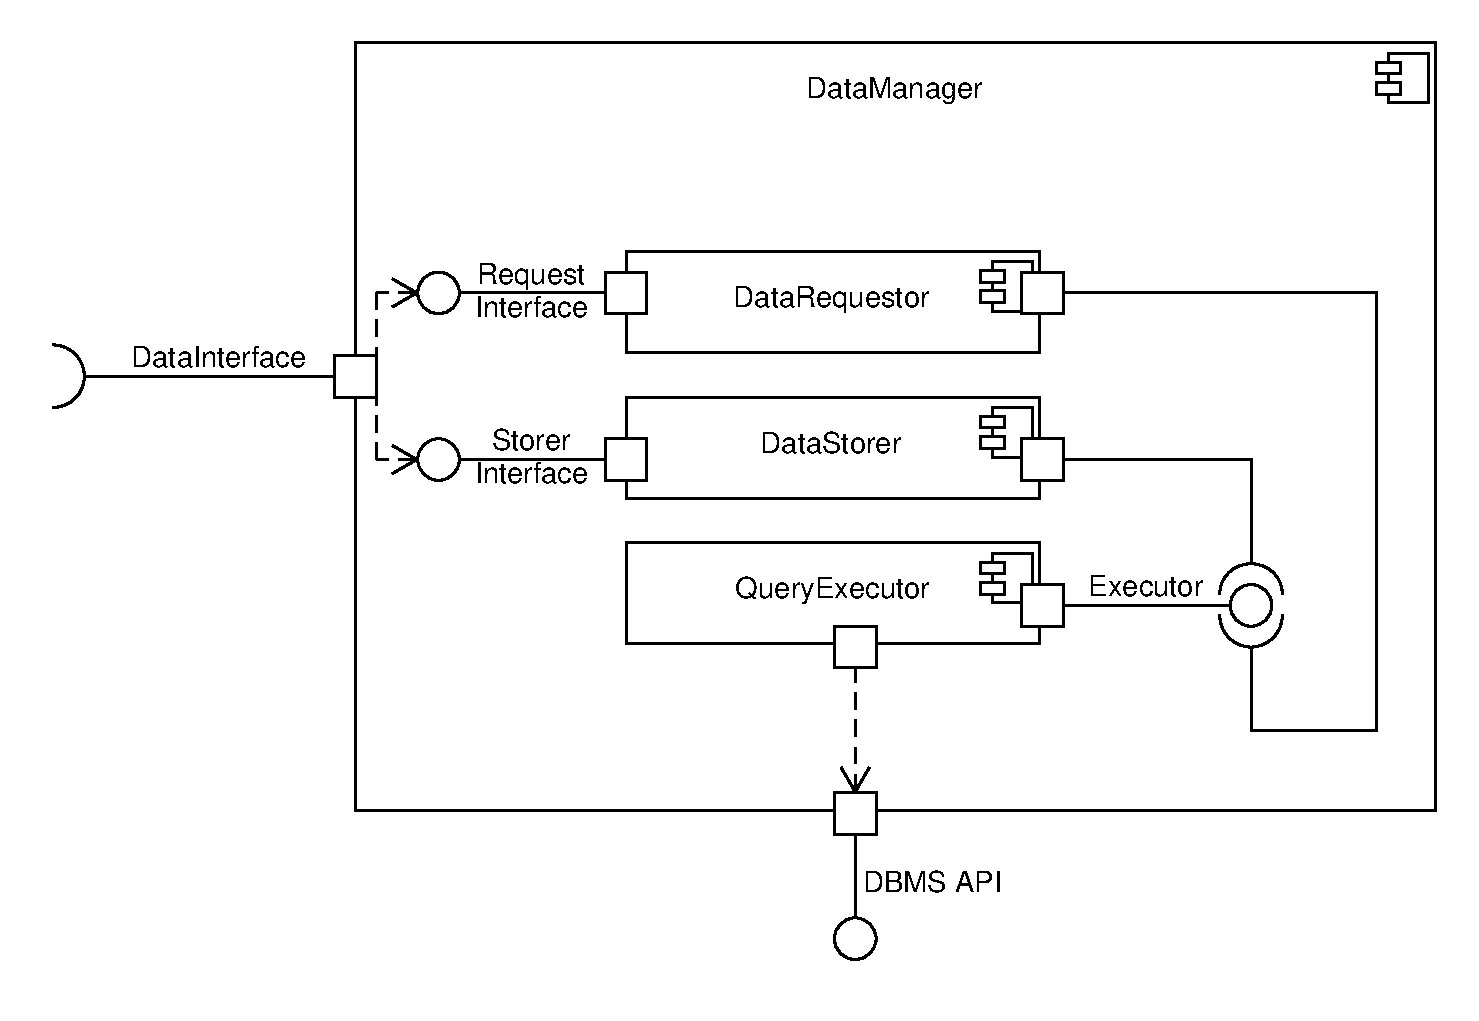
\includegraphics[scale=0.5]{Component Diagrams/DataManagerComponentView.pdf}\\
					\end{adjustwidth}
					\caption{\emph{Data Manager Component View}}
				\end{figure}
			
			\subsubsection{CLup Server}
			As said before, it manages customers’ requests and access operations, through the two interfaces it expose:
			
			\begin{itemize}
				\item {\bfseries CustomerInterface}: expose all the methods relative to services a customer can access, such as making a reservation and retrieving already made reservations.
				
				\item {\bfseries AccessManager}: the interface deputy to manage login and registration of users. After a login, will send to the user the correct set of operations the user can do, depending on their role: customers or store managers.
			\end{itemize}
			
			In the following paragraphs, there is a description of the most relevant component contained in {\bfseries CLup Server}.
			\begin{figure}
				\begin{adjustwidth} {0cm}{}
					\centering
					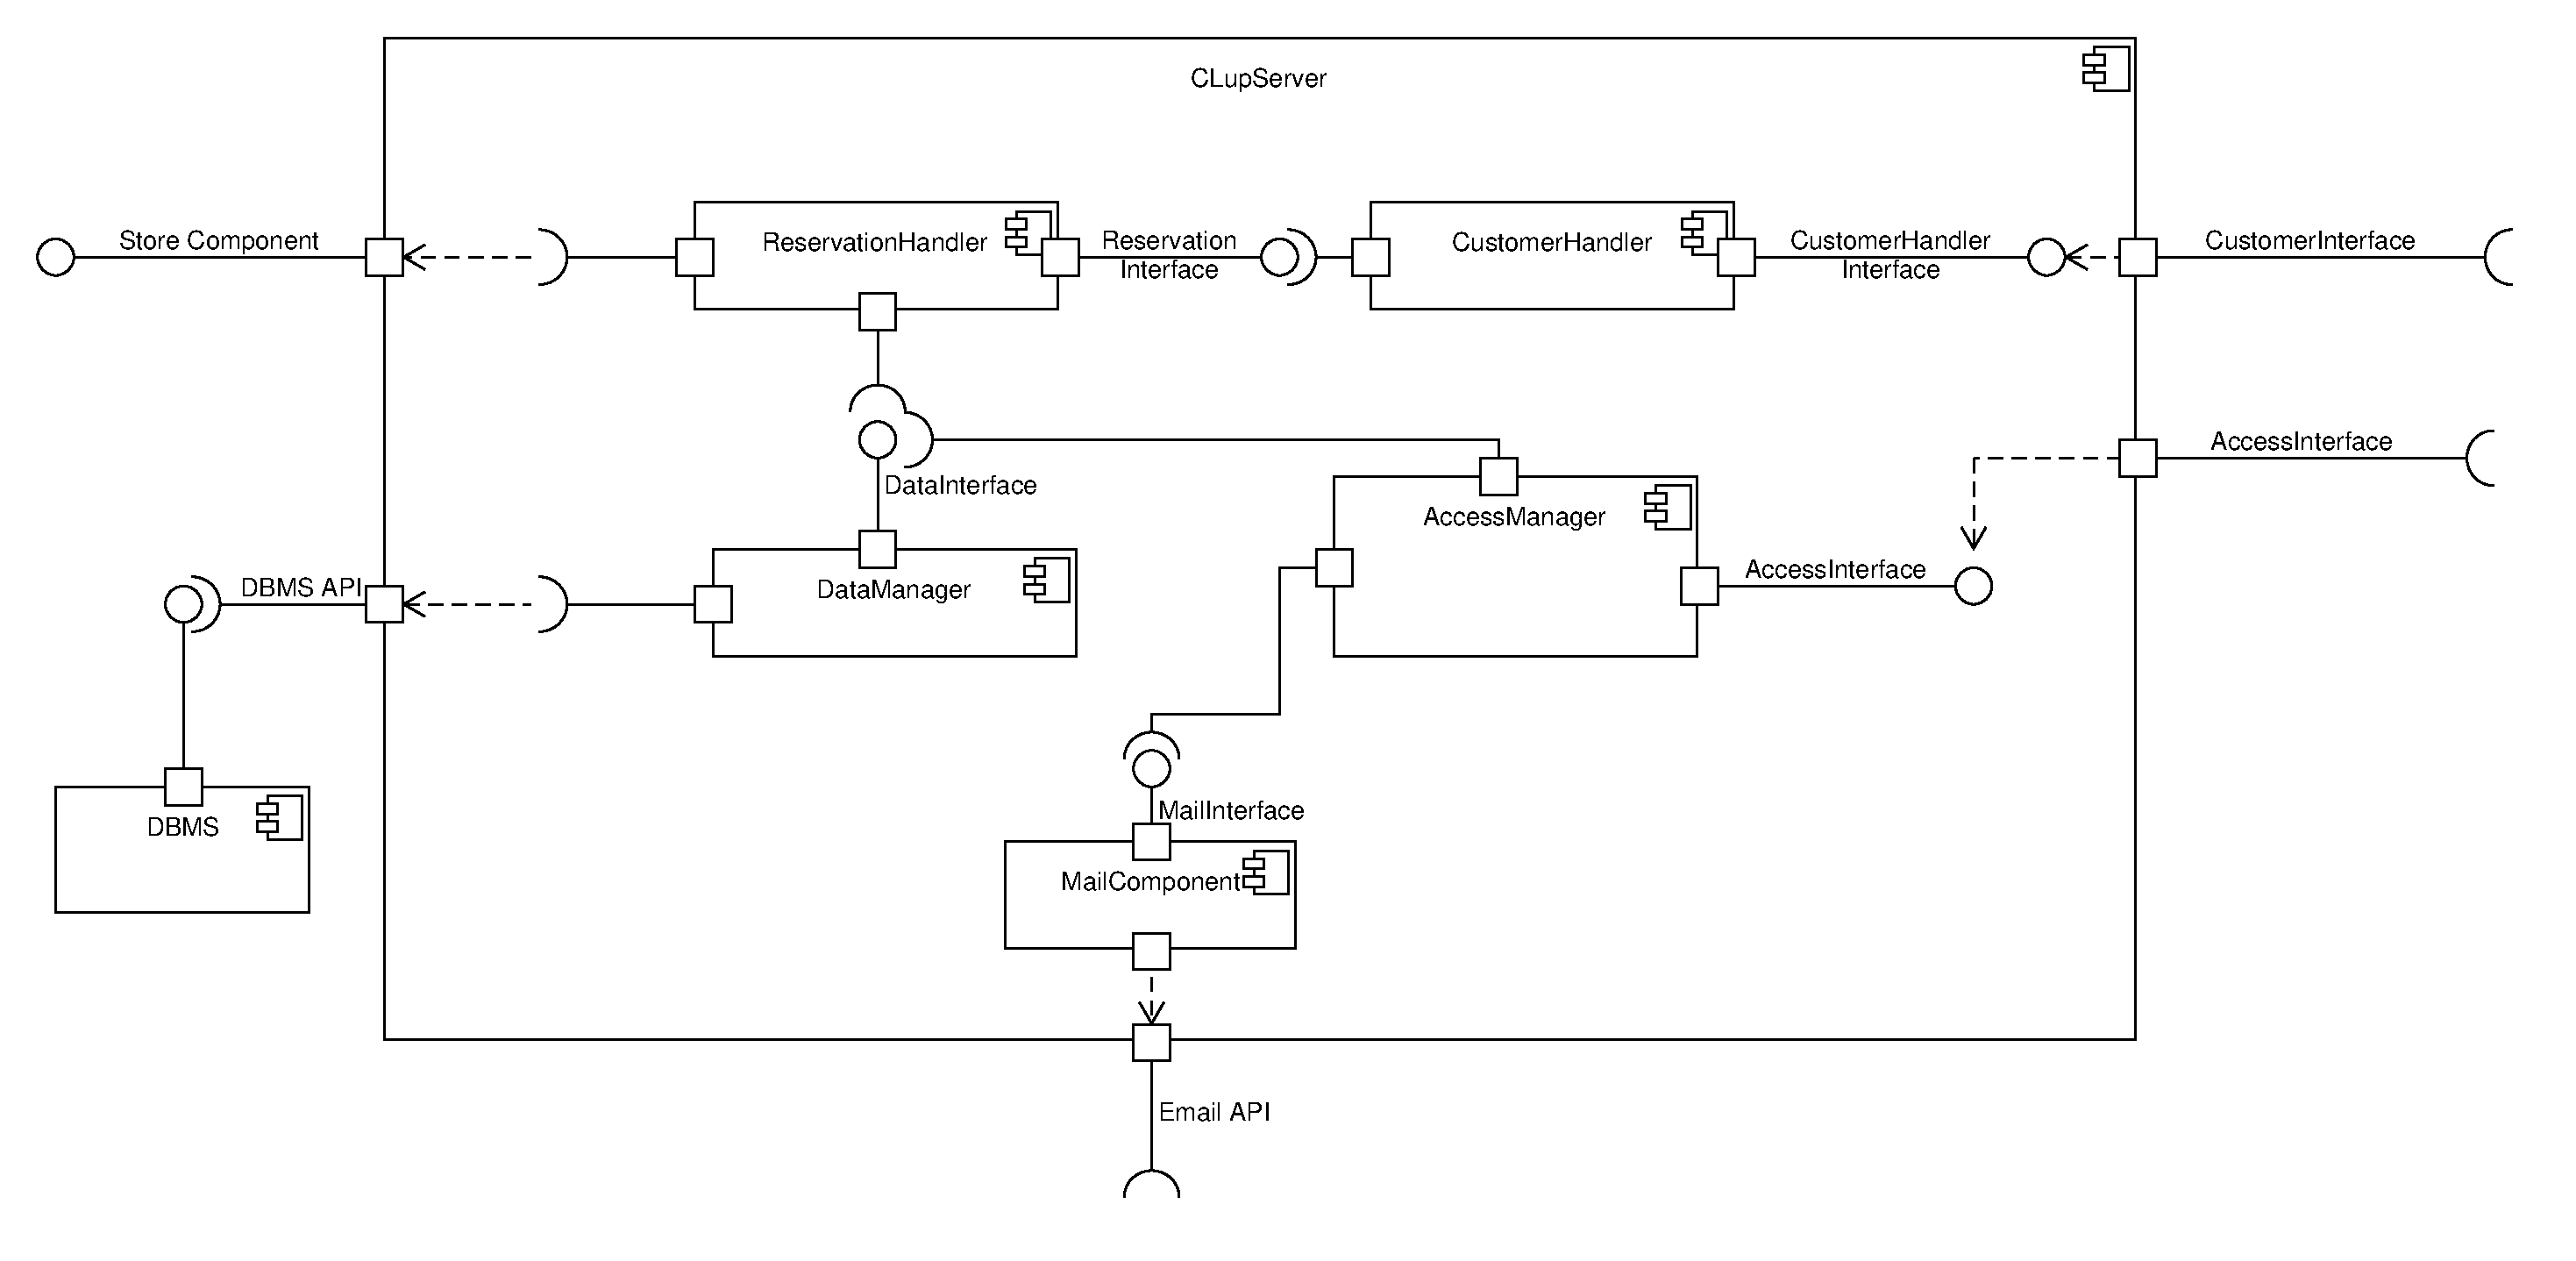
\includegraphics[scale=0.37, angle=90, trim= 0 0 0 -5cm]{Component Diagrams/ServerComponentView.pdf}\\
				\end{adjustwidth}
				\caption{\emph{Server Component View}}
			\end{figure}
			\newpage
				\paragraph{Customer Handler Component}
					The CustomerHandler is the component that manages all the actions that a customer can make within the application. The component analyze the aspects concerning reservations.
					
					This component is used by invoking methods on the \emph{CustomerHandlerInterface}. This component is divided in some subcomponents:
					
					\begin{itemize}
						\item {\bfseries ASAPManager}: it is the component that manages the \emph{ASAP} reservations and it is formed from two sub-component: {\bfseries DeleteRes} and {\bfseries AddRes}. The first one deals with deleting an \emph{ASAP} reservation while the second one deals with creating a new \emph{ASAP} reservation.
						
						\item {\bfseries BookingManager}: it is the component that manages the booking via app and it is formed from three sub-component: {\bfseries DeleteRes}, {\bfseries ModifyRes} and {\bfseries AddRes}. The first one deals with deleting a reservation, the second one deals with modifying a reservation while the third one deals with adding new reservations. 
						
						\item {\bfseries RetriveReservation}: it is the component that is used to retrieve and update all user’s reservations.
					\end{itemize}
				
					All of these components uses the \emph{ReservationInterface} to complete their tasks.
					\bigskip
					\begin{figure}[h]
						\begin{adjustwidth} {-4cm}{}
							\centering
							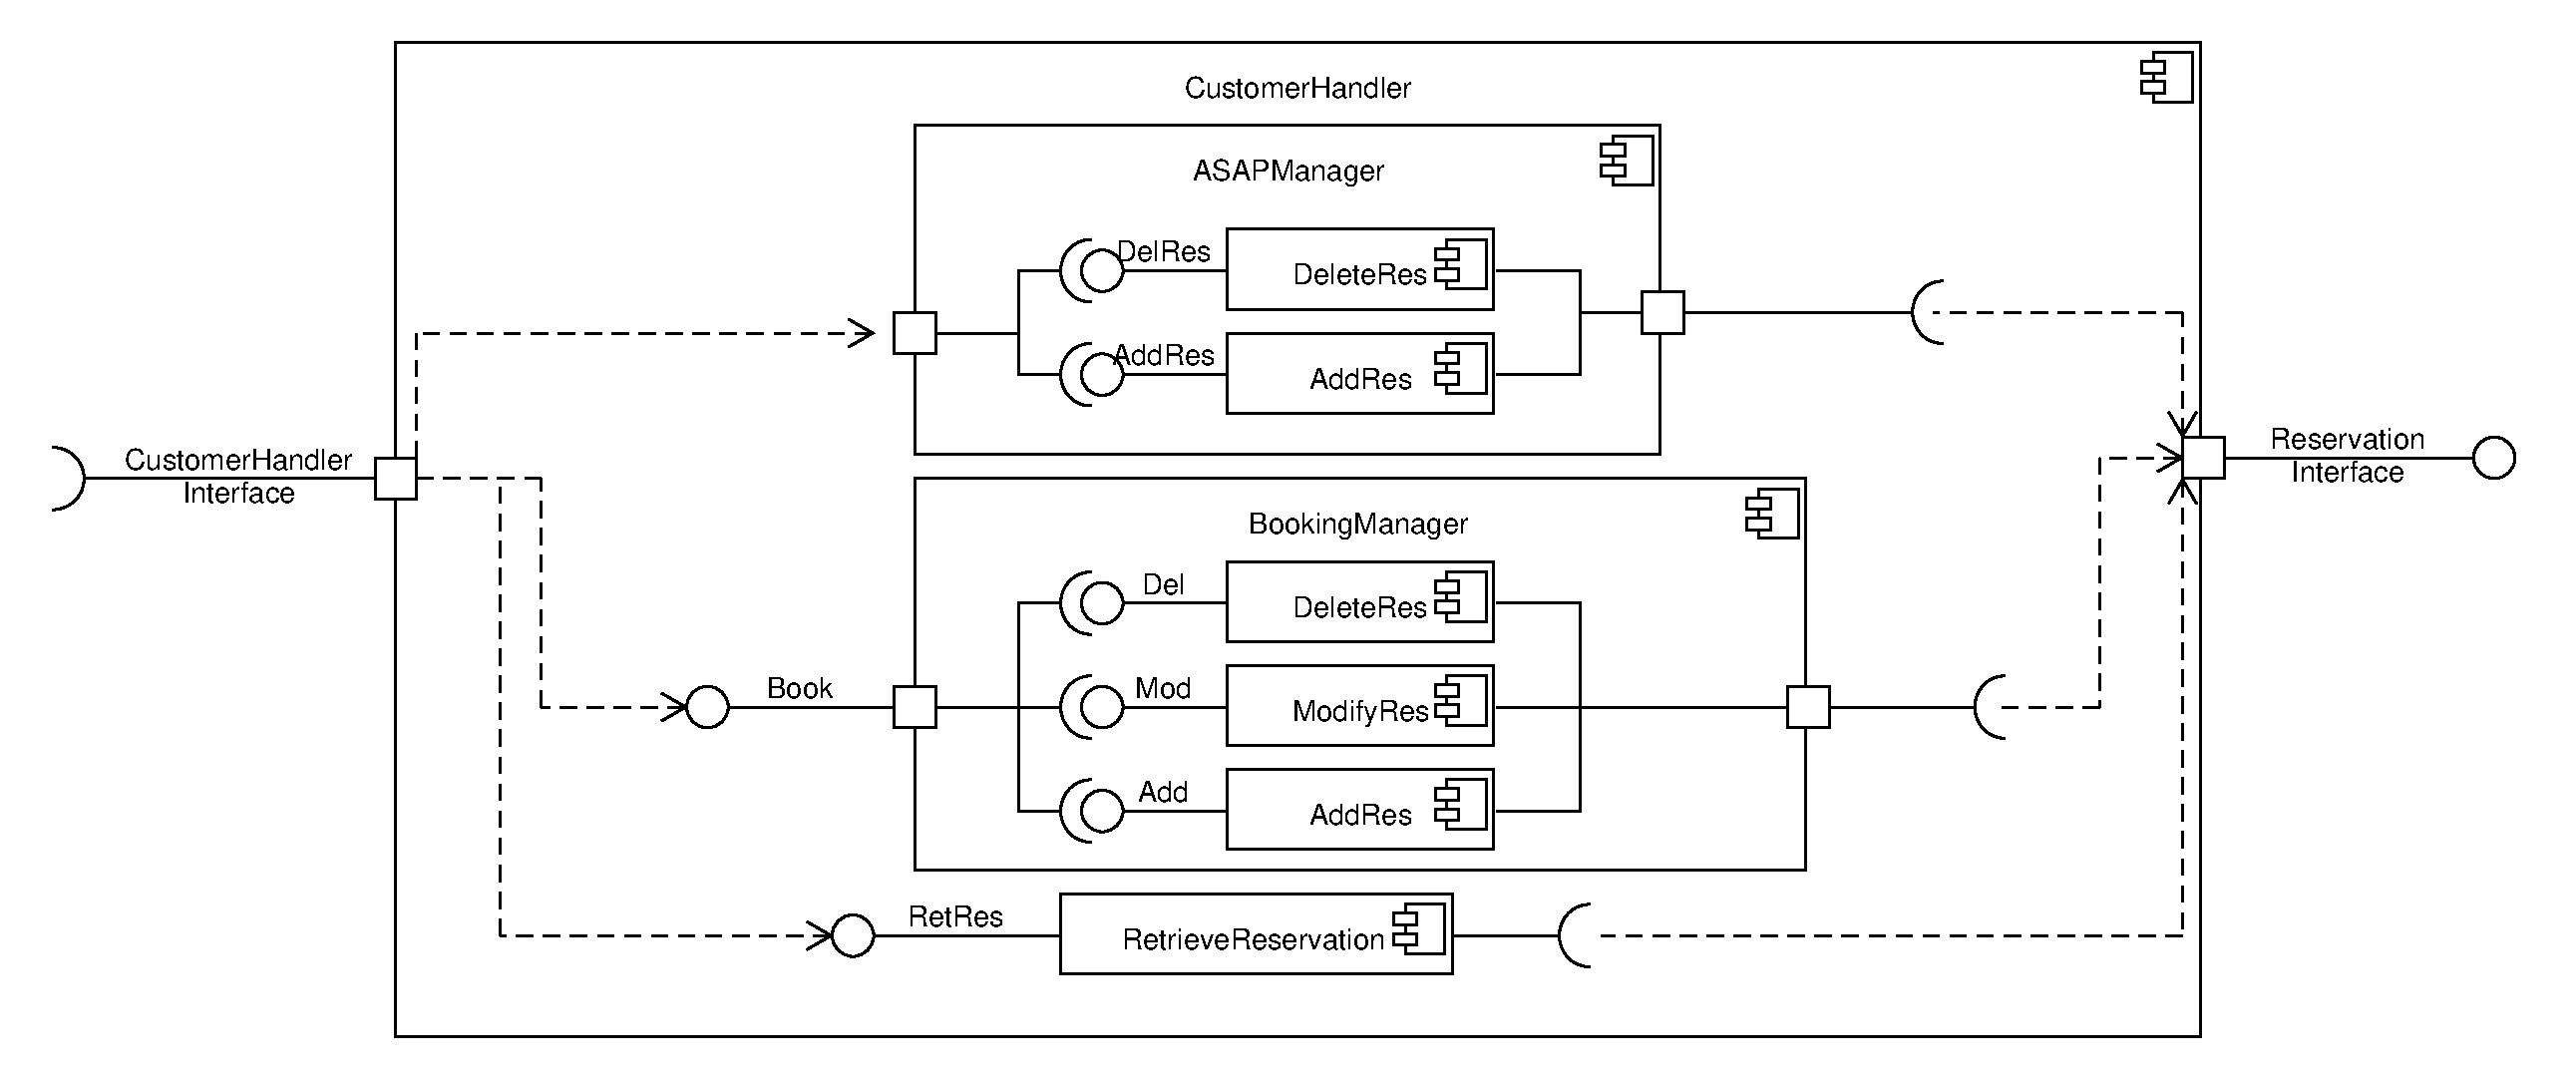
\includegraphics[scale=0.45]{Component Diagrams/CustomerHandlerComponentView.pdf}\\
						\end{adjustwidth}
						\caption{\emph{Customer Handler Component View}}
					\end{figure}
				\newpage
				\paragraph{Access Manager Component}
					The Access Manager is the component that manages all the issues concerning the access of the users. Indeed, as mentioned above, it is very important to recognize the role of the users in the app in order to provide them correct information, and only the functionalities/data they are authorized to use. The component analyze two main aspects:
					
					\begin{itemize}
						\item Login
						\item Registration
					\end{itemize}
				
					The component uses two very important interfaces: \emph{EmailAPI} and \emph{DataInterface}. The first one is used for the registration, in order to send confirmation messages, while the second one is used for storing registration data, and to check credentials for log-in operations. Furthermore, its services are requested through the \emph{AccessInterface}, that implements the interfaces exposed by {\bfseries Login Component}, and {\bfseries Registration Component}. This component is invoked by \emph{StoreManageAccessInterface} and \emph{CustomerAccessInterface} in case an user wants to log in or register
					
					\begin{itemize}
						\item {\bfseries LoginManager}: it is the component that manages user’s login. Indeed, if a user logs in, the component checks if the credentials are correct and then allows the user to use their personal area.
						
						\item {\bfseries RegistrationManager}: it is the component that manages the user’s registration. Indeed, if a user makes a registration, this component, at the beginning, checks through \emph{DataInterface} if the data inserted by the user are valid (e.g. uniqueness of the email, or certification for store managers). Then, if the data are correct, the user’s data are stored in the \emph{DBMS}.
						
						\begin{itemize}
							\item {\bfseries RegistrationChecker}: it is the component that checks if the information is inserted during the registration, from the user, are valid. In case of customers, this component checks if the email is valid while in case of store manager checks if the store certification is valid and the registration \emph{ID} is unique.
							
							\item {\bfseries RegistrationStorer}: it is the component that stores the new data in the \emph{DBMS} after checking.
						\end{itemize}
					\end{itemize}
				
				\begin{figure}[h]
					\begin{adjustwidth} {-2.5cm}{}
						\centering
						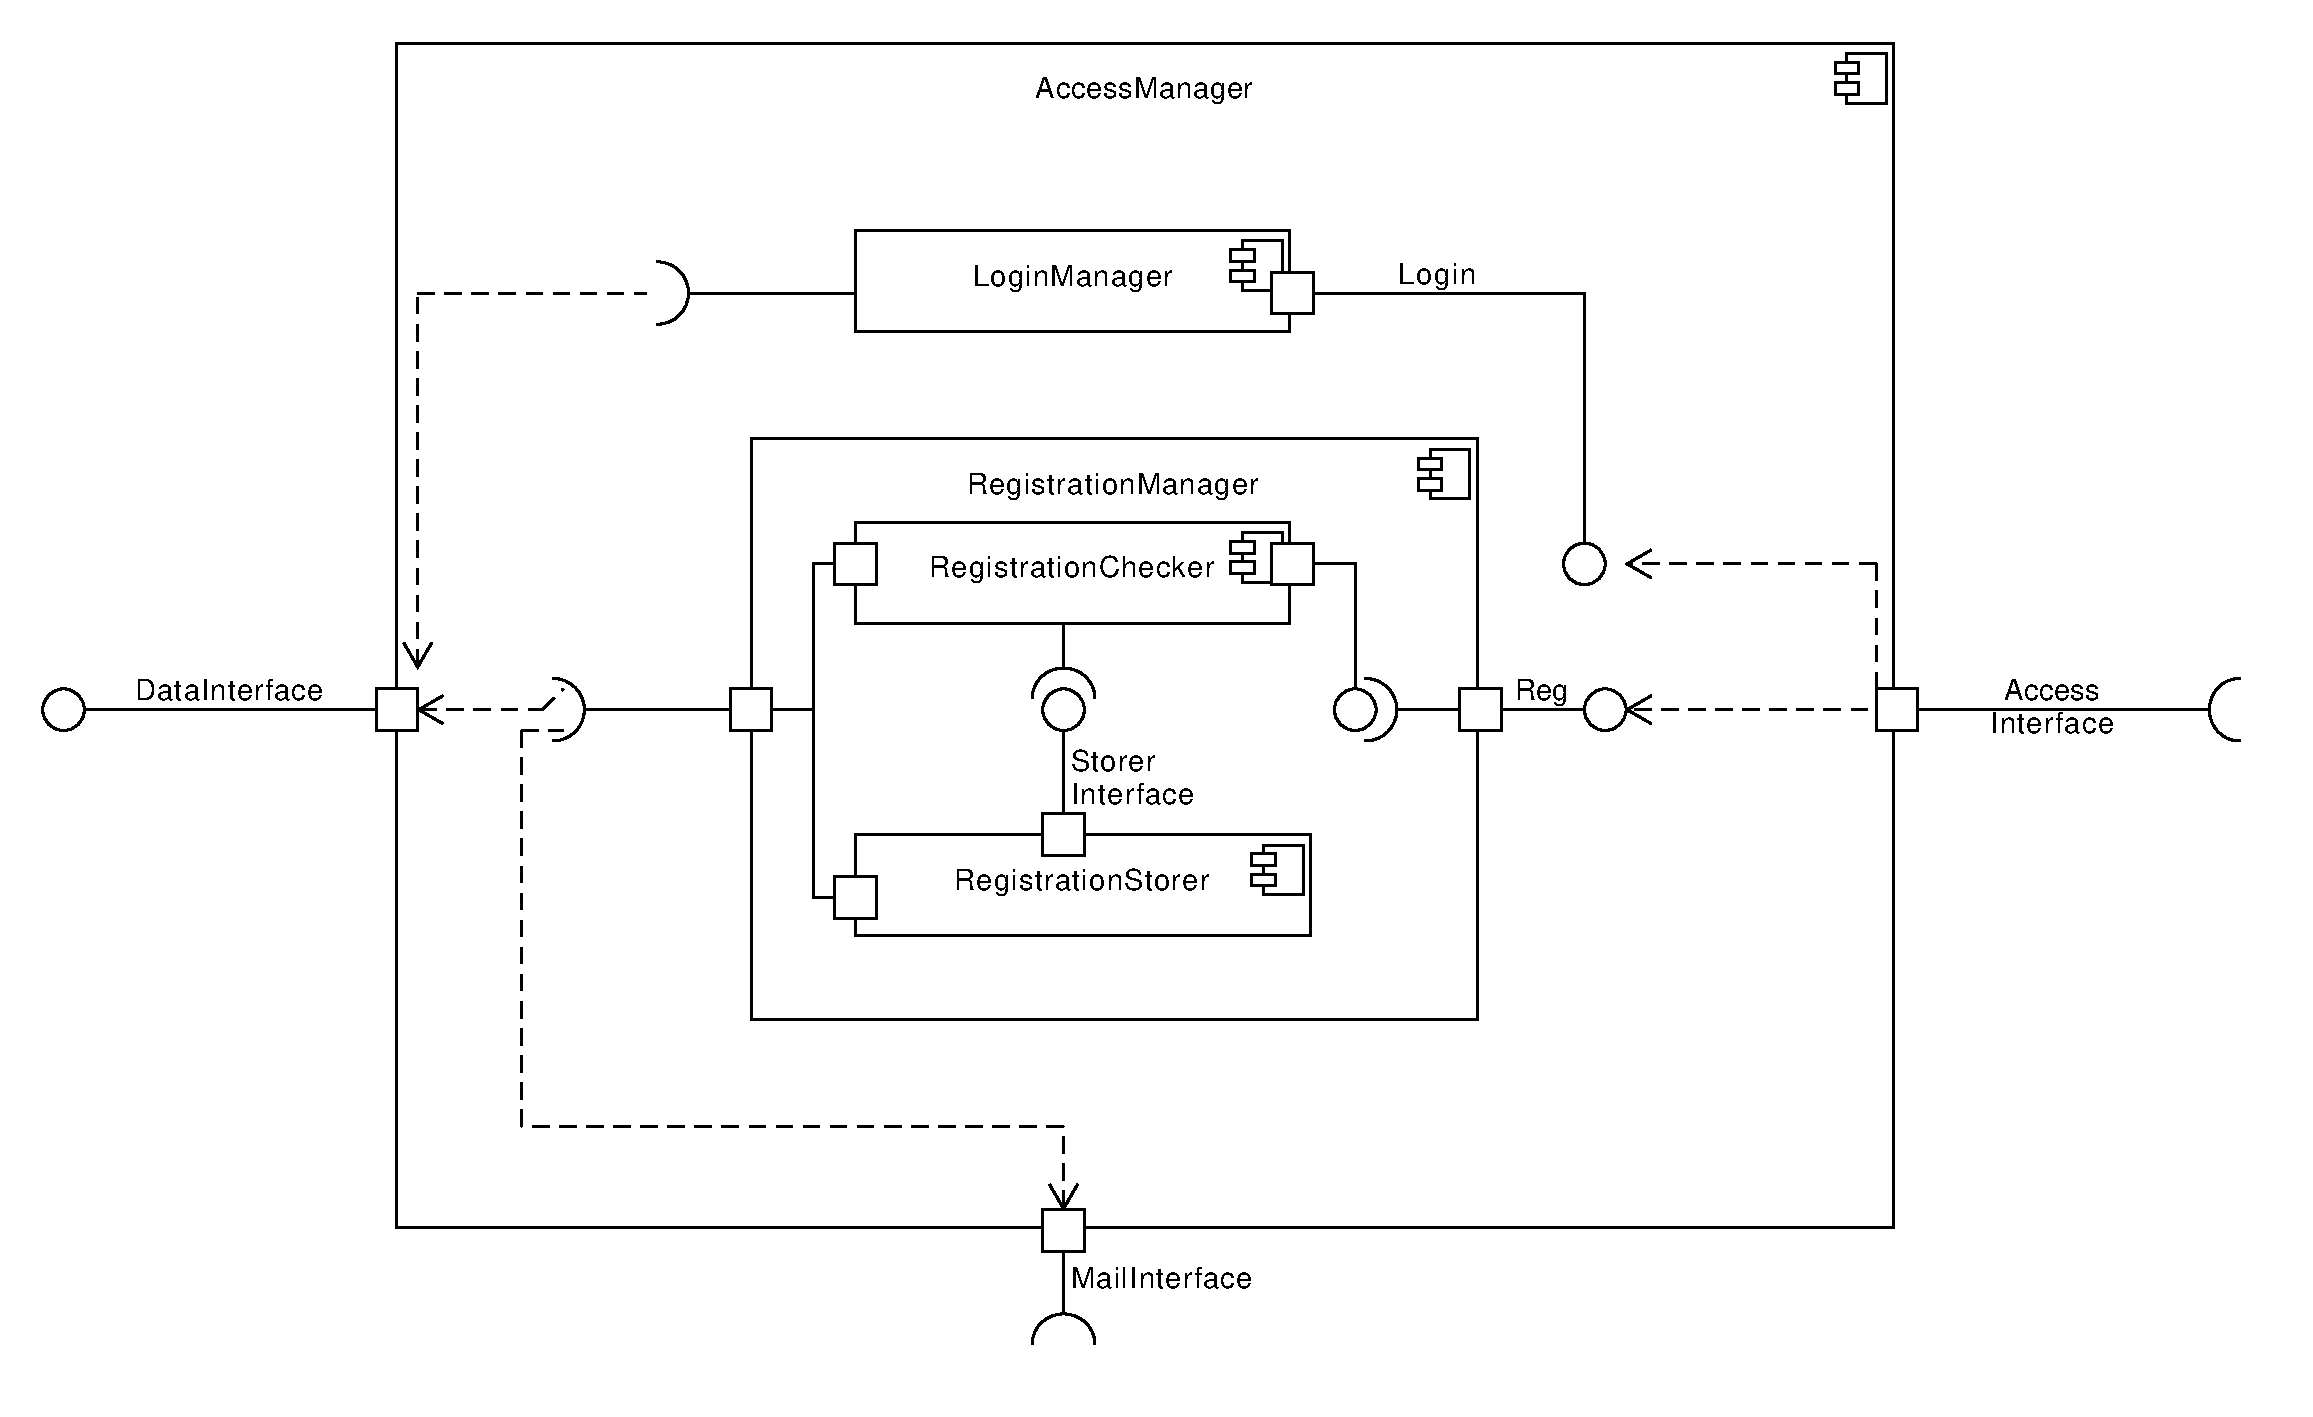
\includegraphics[scale=0.45]{Component Diagrams/AccessManagerComponentView.pdf}\\
					\end{adjustwidth}
					\caption{\emph{Access Manager Component View}}
				\end{figure}
				\newpage
				
			\paragraph{Reservation Handler Component}
				The Reservation Handler is the component that manages the customer’s reservations. The component analyzes two main aspects:
				
				\begin{itemize}
					\item Suggestions
					\item Reservation Management
				\end{itemize}
			
				The component uses \emph{ReservationInterface} (that implements \emph{QueryInterface} and \emph{SuggestionInterface}) to accept requests that are processed by this component , and {\bfseries Store Component}, used to make requests to a specific store.
				This component is invoked when the customer tries to make or modify a reservation, or tries to retrieve his ones. Each time a reservation is retrieved, the customer will receive the updated information (such us \emph{ETA} to enter the store).
				
				\begin{itemize}
					\item {\bfseries SuggestionComponent}: it is the component that manages the suggestions that are made available to the customer at the time of reservation. It will query each store registered on the platform, to retrieve availability information, depending on the preferences inserted by the customer and the type of reservation they are making (so, the component will use the right {\bfseries Query Component}); it’s invoked by both the \emph{ReservationInterface} when a customer asks for suggestions on bookings, or by {\bfseries ASAPQueryComponent} while the \emph{ETA} for entering the store \emph{ASAP} is too high.
					
					\item {\bfseries StoreQueryComponent}: it is the component that manages the queries that are made at a particular store, indeed this component uses the {\bfseries Store Component}. The queries they can be of two types:
					
					\begin{itemize}
						\item {\bfseries ASAPQueryComponent}: it is the component that manages the \emph{ASAP} reservation, asks the server for waiting times for accessing the store, notifies the store if a reservation is made and manage the deletion of \emph{ASAP} reservations.
						
						\item {\bfseries BookingQueryComponent}: it is the component that manages the booking via app, asking the server time slots to enter the store, in case a reservation is confirmed, notify the store to save it, and manage all the requests about modification and cancellation of booking reservations.		
					\end{itemize}
				\end{itemize}
				\bigskip
				\begin{figure}[h]
					\begin{adjustwidth} {-0.5cm}{}
						\centering
						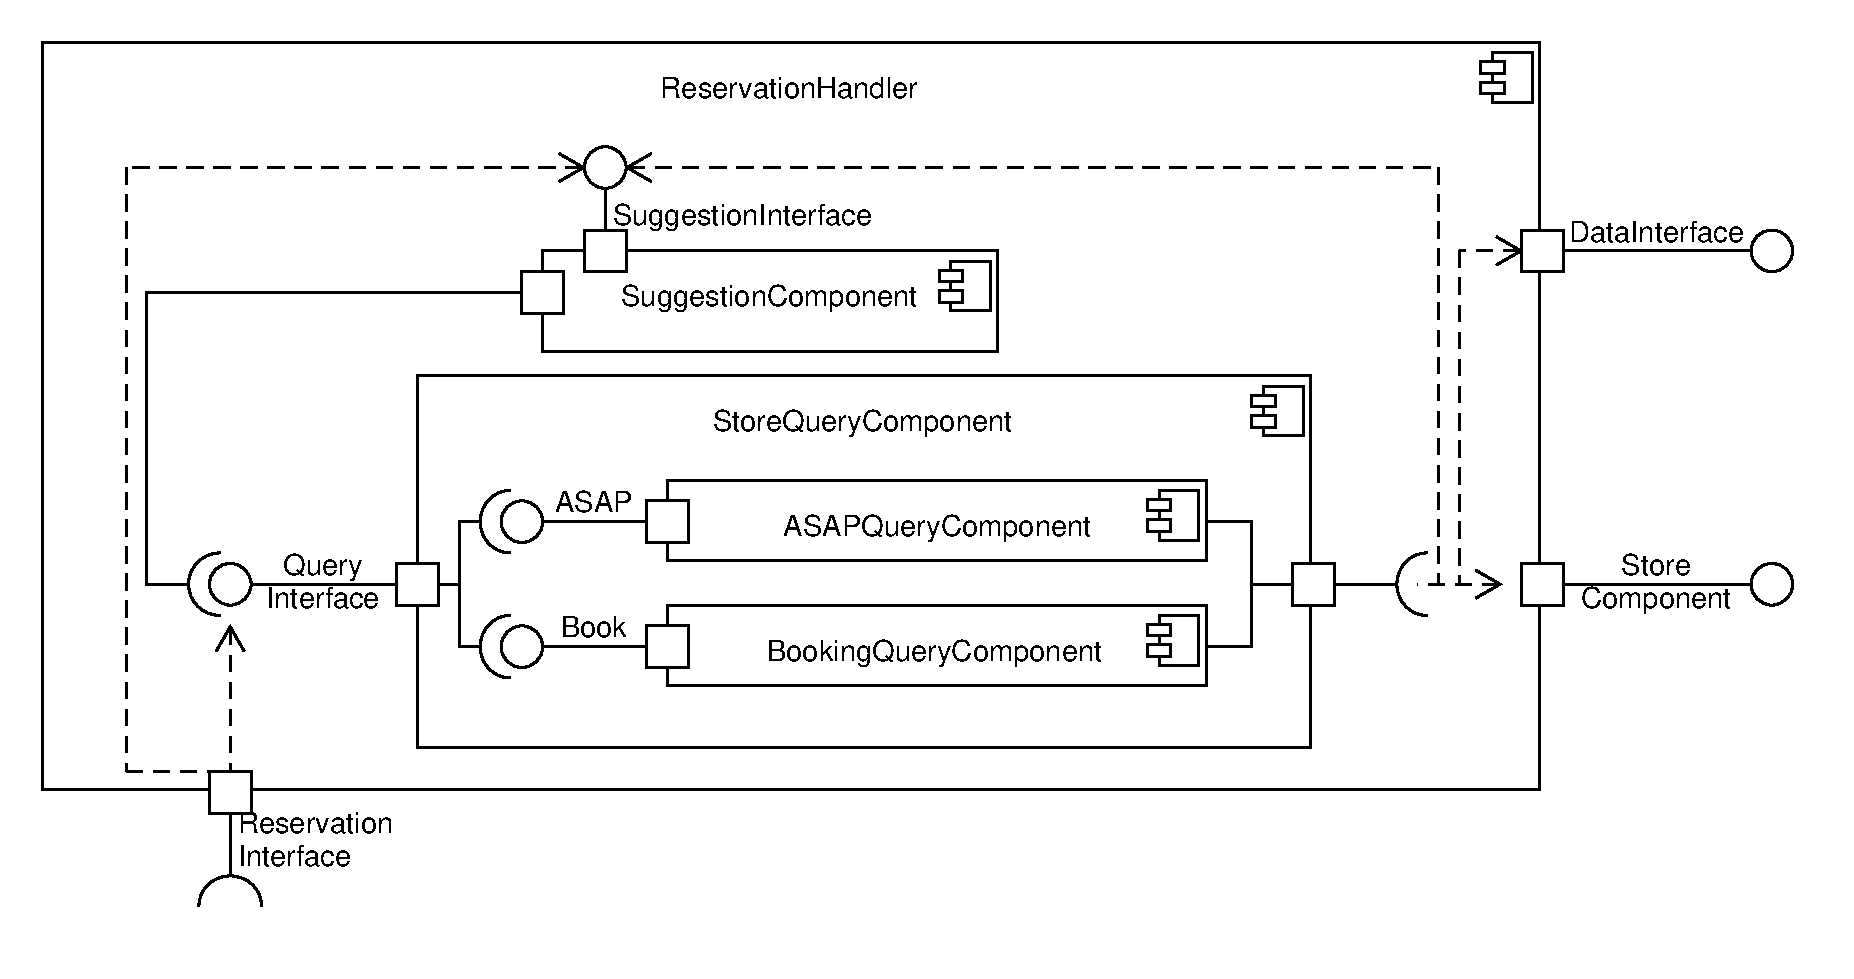
\includegraphics[scale=0.5]{Component Diagrams/ReservationHandlerComponentView.pdf}\\
					\end{adjustwidth}
					\caption{\emph{Reservation Handler Component View}}
				\end{figure}
				\newpage
			
		\subsubsection{Store Component}
			The Store is the component that manages the store from all points of view and it is the most important component of the whole architecture, since implements the whole business tier. The component analyze many important aspect, but the most important are:
			
			\begin{itemize}
				\item Reservation
				\item Admit Reservations Inside
				\item Store Parameters
				\item Statistical Values
			\end{itemize}
		
			As said before, it’s been preferred to separate the logic governing each store by designing a component for each different store. Also here, the store component have been designed in a modular way, to separate the different features offered by a single store; these are:
			
			\begin{itemize}
				\item {\bfseries FlowComponent}: this component manages the functionalities that are requested when a \emph{QR Code} is scanned at the store entry, and uses the {\bfseries Calling Number Component} to authorize the entry, and uses the {\bfseries Department Component} to register the entrance/exit.
				
				\item {\bfseries StatisticComponent}: it is the component dedicated to building customer statistics. It’s used by:
				
				\begin{itemize}
					\item {\bfseries EntranceComponent}: in order to update visiting statistics at customers’ exit
					\item {\bfseries ReservationComponent}: invokes the methods when, during a reservation process, it’s necessary to infer the estimation of customers’ shopping time.
				\end{itemize}
			
				\item {\bfseries RearrangeComponent}: it is the component that rearrange the reservations when a store manager modifies the capacity of some part of the store. Interacts with the {\bfseries Calling Number Component} in order to rearrange the queue. In case of delays or cancellations, the customers will receive a notification.
				
				\item {\bfseries StoreDataManager}: it is the adapter between the store and its dedicated \emph{DBMS}. The choice of dedicating a \emph{DBMS} for each store is due to efficiency and security reasons: if a \emph{DBMS} broke, it wouldn't affect the whole system, while a store can access only its data.
				
				\item {\bfseries ParameterManager}: it is the component that manages the parameters of the store, the settings and the situation of each department of the store. It’s used by:
				
				\begin{itemize}
					\item {\bfseries EntranceComponent}: is used to update Departments’ situation.
					\item {\bfseries StoreManagerHandler}: is used to update store parameters, and to access the real-time situation of the store.
				\end{itemize}
			
				Moreover, uses {\bfseries RearrangeReservation} when a parameter is modified, to make coherent the store’s status
				
				\item {\bfseries ReservationComponent}: it is the component that is dedicated to the management of reservations. It’s used to retrieve reservations made in that store, to retrieve waiting times, and to store customers’ reservations. Uses the {\bfseries Calling Number Component} to notify the creation of a new reservation, and it’s used by the latter to initialize the queue at store opening. It also handles modifications made by customers and store managers to reservations. Furthermore, a store manager uses it to contact customers about some specific reservation. Because of this, the components interact with {\bfseries Notification Component} and {\bfseries Mail Component} to interact with customers. 
				To logically separate the management of the two types of reservations, the component is divided in two subcomponents: {\bfseries BookingComponent}, and {\bfseries ASAPComponent}.
				
				\item {\bfseries CallingNumberComponent}: it is the component deputy to call in reservations, and to notify customers they should depart for the store. To do this, it interfaces with \emph{MapInterface} to calculate travel time, and with \emph{NotificationInterface} to send customers notification. It’s divided in two subcomponents, each carrying out different functionalities:
				
				\begin{itemize}
					\item {\bfseries CallableReservationComponent}: checks whenever a reservation in the queue is callable, checking the store affluence, through the {bfseries Parameter Manager Component}; when it notice that a customer should be alerted to depart for the store, sends a notification through the {\bfseries Notification Manager Component}.
					
					\item {\bfseries CallNumberComponent}: takes a queue of reservations to be called, and when it’s possible, a reservation is called to enter. It’s alerted by the {\bfseries Entrance Component} that somebody exited the store.
				\end{itemize}
			\end{itemize}
		
			The core store functionalities are requested through the \emph{ReservationInterface} (dedicated to customers’ features) and the \emph{StoreInterfaces}, dedicated to store managers; their requests pass through an handler, here described. One note: the \emph{StoreComponentInterfaces} implements all the interfaces of the single services requested by the {\bfseries Store Manager Handler}.
			
			\begin{figure}[H]
				\begin{adjustwidth} {-1cm}{}
					\centering
					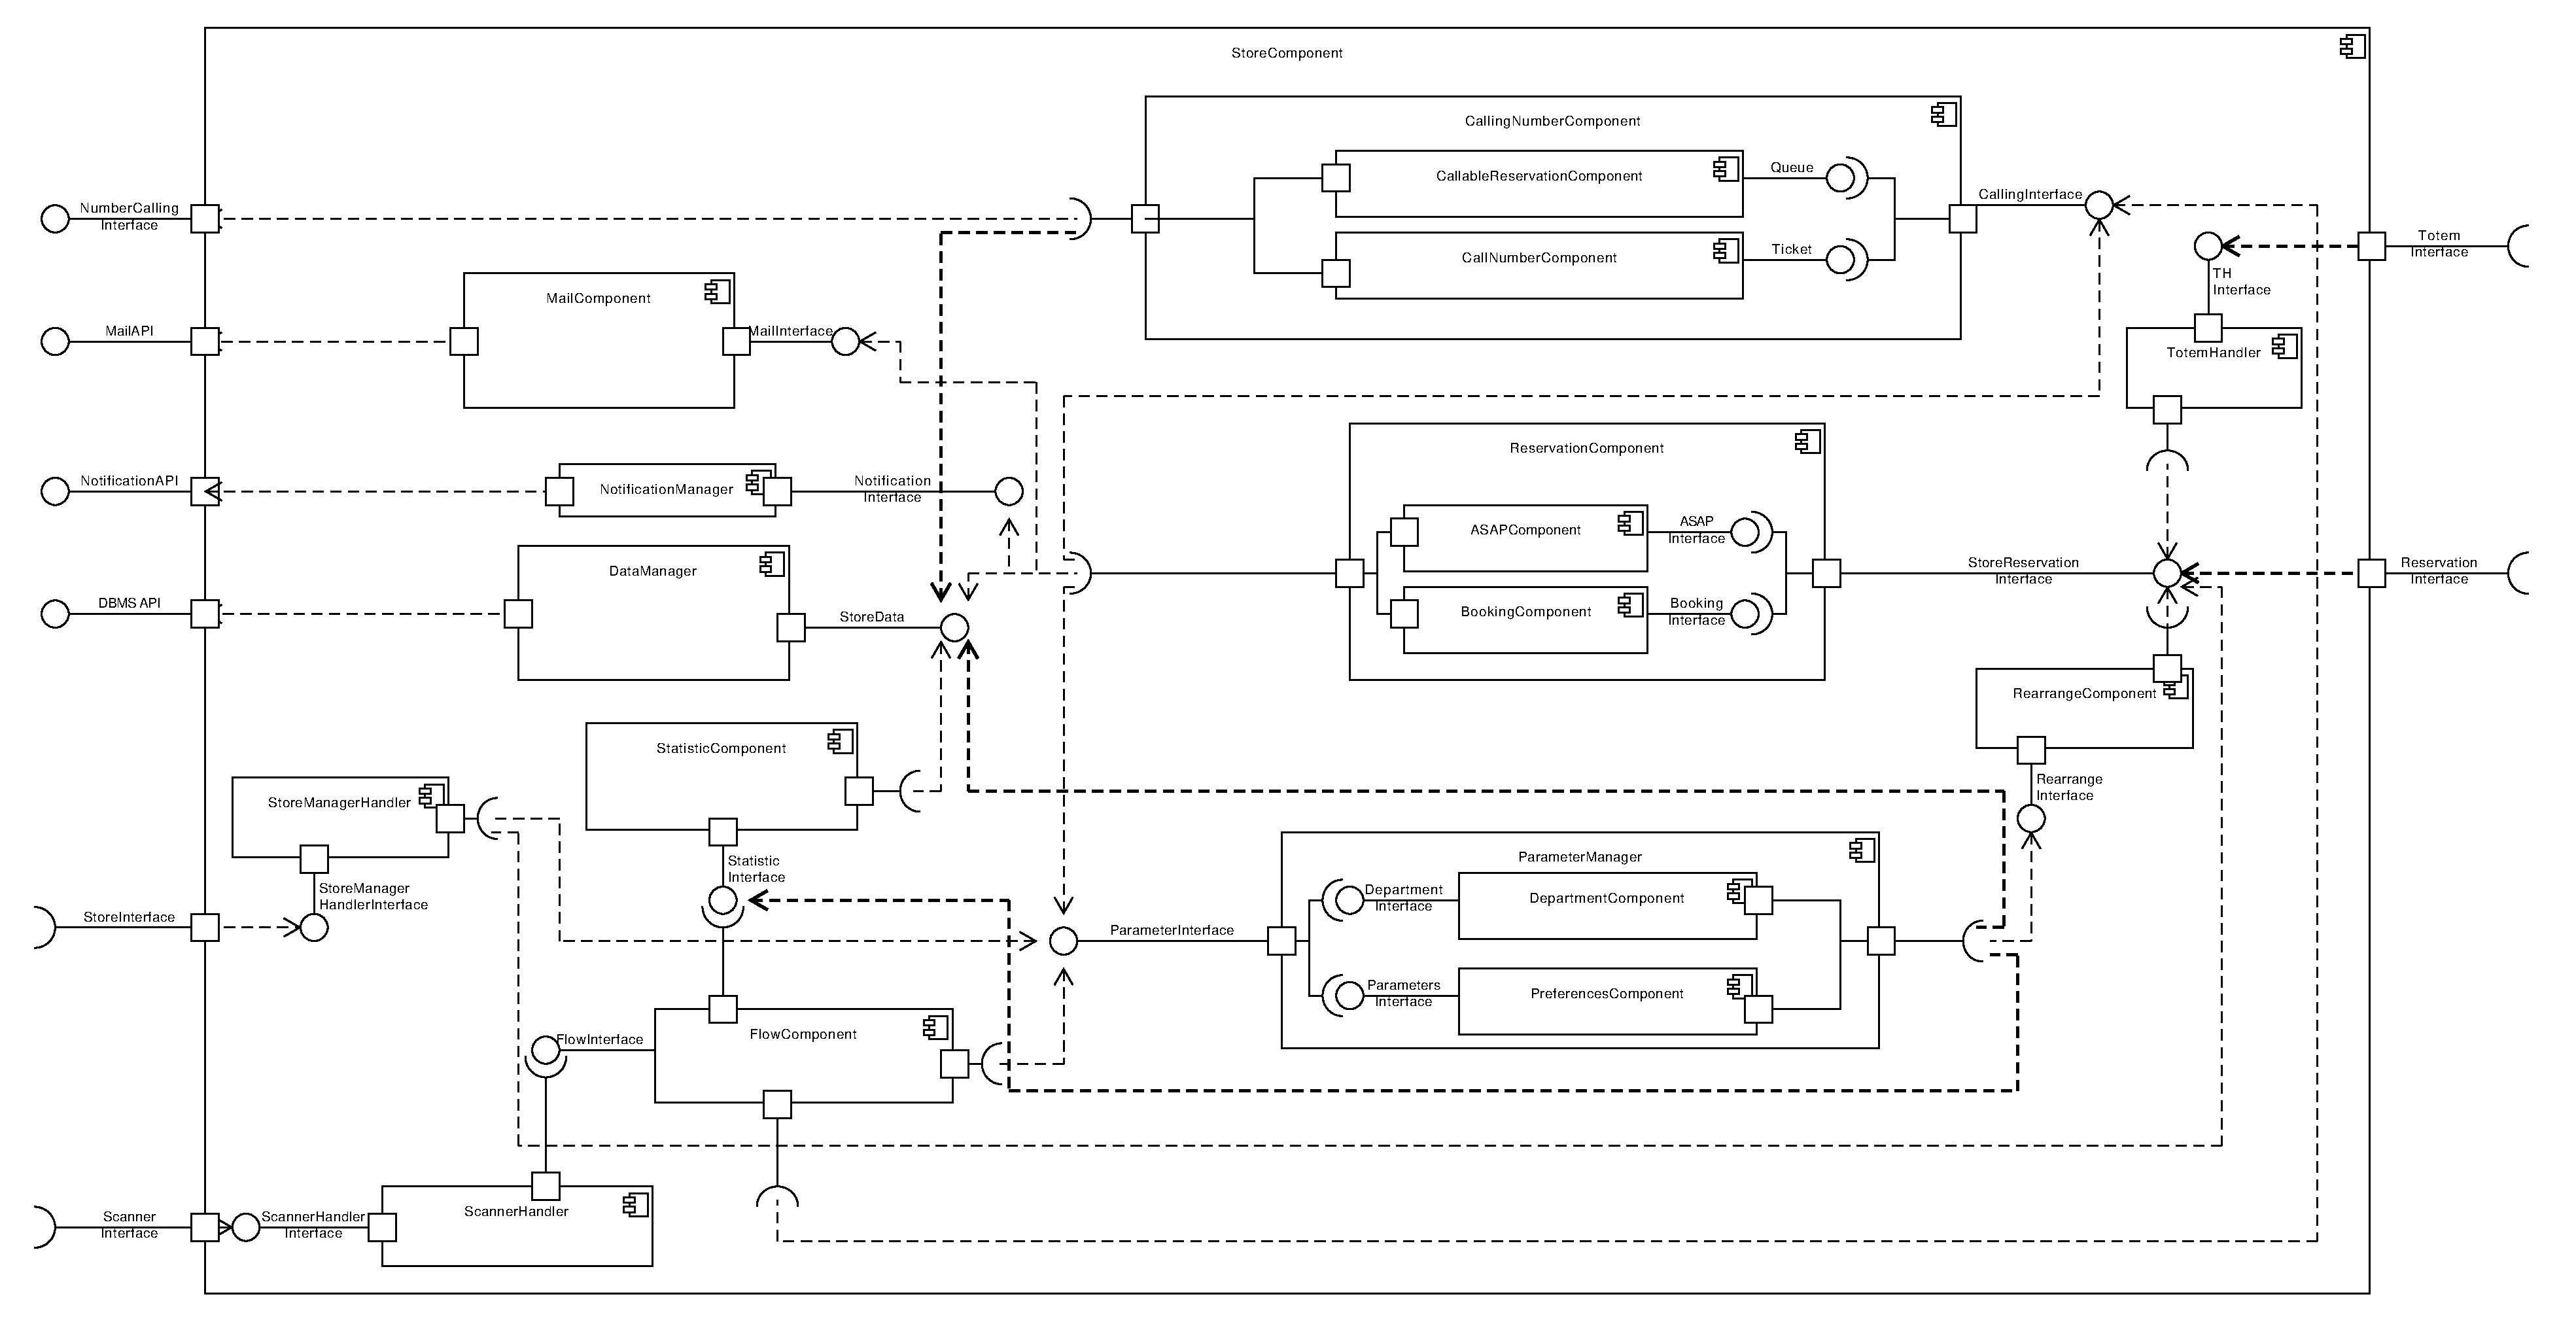
\includegraphics[scale=0.22, angle=90, trim= 0 0 0 -5cm]{Component Diagrams/ReorderedStoreComponentView.pdf}\\
				\end{adjustwidth}
				\caption{\emph{Store Component View}}
			\end{figure}
			\newpage
			
		\subsubsection{Store Manager Handler Component}
			The Store Manager Handler is the component that manages all the actions that a store manager can make within the application. The component analyze various aspects:
			
			\begin{itemize}
				\item Reservations
				\item Modify Parameters
			\end{itemize}
		
			This component handles all the possible settable options of a store manager, it is invoked on the \emph{StoreInterface}, from the mobile application, and it interfaces with \emph{StoreComponentInterface}, that manages all information regarding parameters and reservations.
			
			\begin{itemize}
				\item {\bfseries ManagerReservationHandler}: it is the component that manages the store reservations and it is divided in two sub-component:
				
				\begin{itemize}
					\item {\bfseries DeleteRes}: it is the component that manages the elimination of the reservations.
					\item {\bfseries ModifyRes}: it is the component that manages the modification of the reservations.
				\end{itemize}
				
				\item {\bfseries ModifyParameters}: it is the component that manages the store parameter. They are of two types:
				
				\begin{itemize}
					\item {\bfseries DepartmentManager}: it is the component that manages all the parameters which concern the individual departments. Indeed, the store manager can add or delete a new department and can modify the maximum capacity of each department.
					\item {\bfseries StoreSettingManager}: it is the component that manages all the parameters which concern the entire store. Indeed, the store manager, can change the maximum capacity of the people inside the store and can modify the opening and closing hours.
				\end{itemize}
			
				\item {\bfseries RetriveReservation}: it is the component that manages all the reservation of a specific store.
				
				\item {\bfseries SituationManager}: it is the component that manages the requests for the real time situation of the store.
			\end{itemize}
		
		\begin{figure}[H]
			\begin{adjustwidth} {-4cm}{}
				\centering
				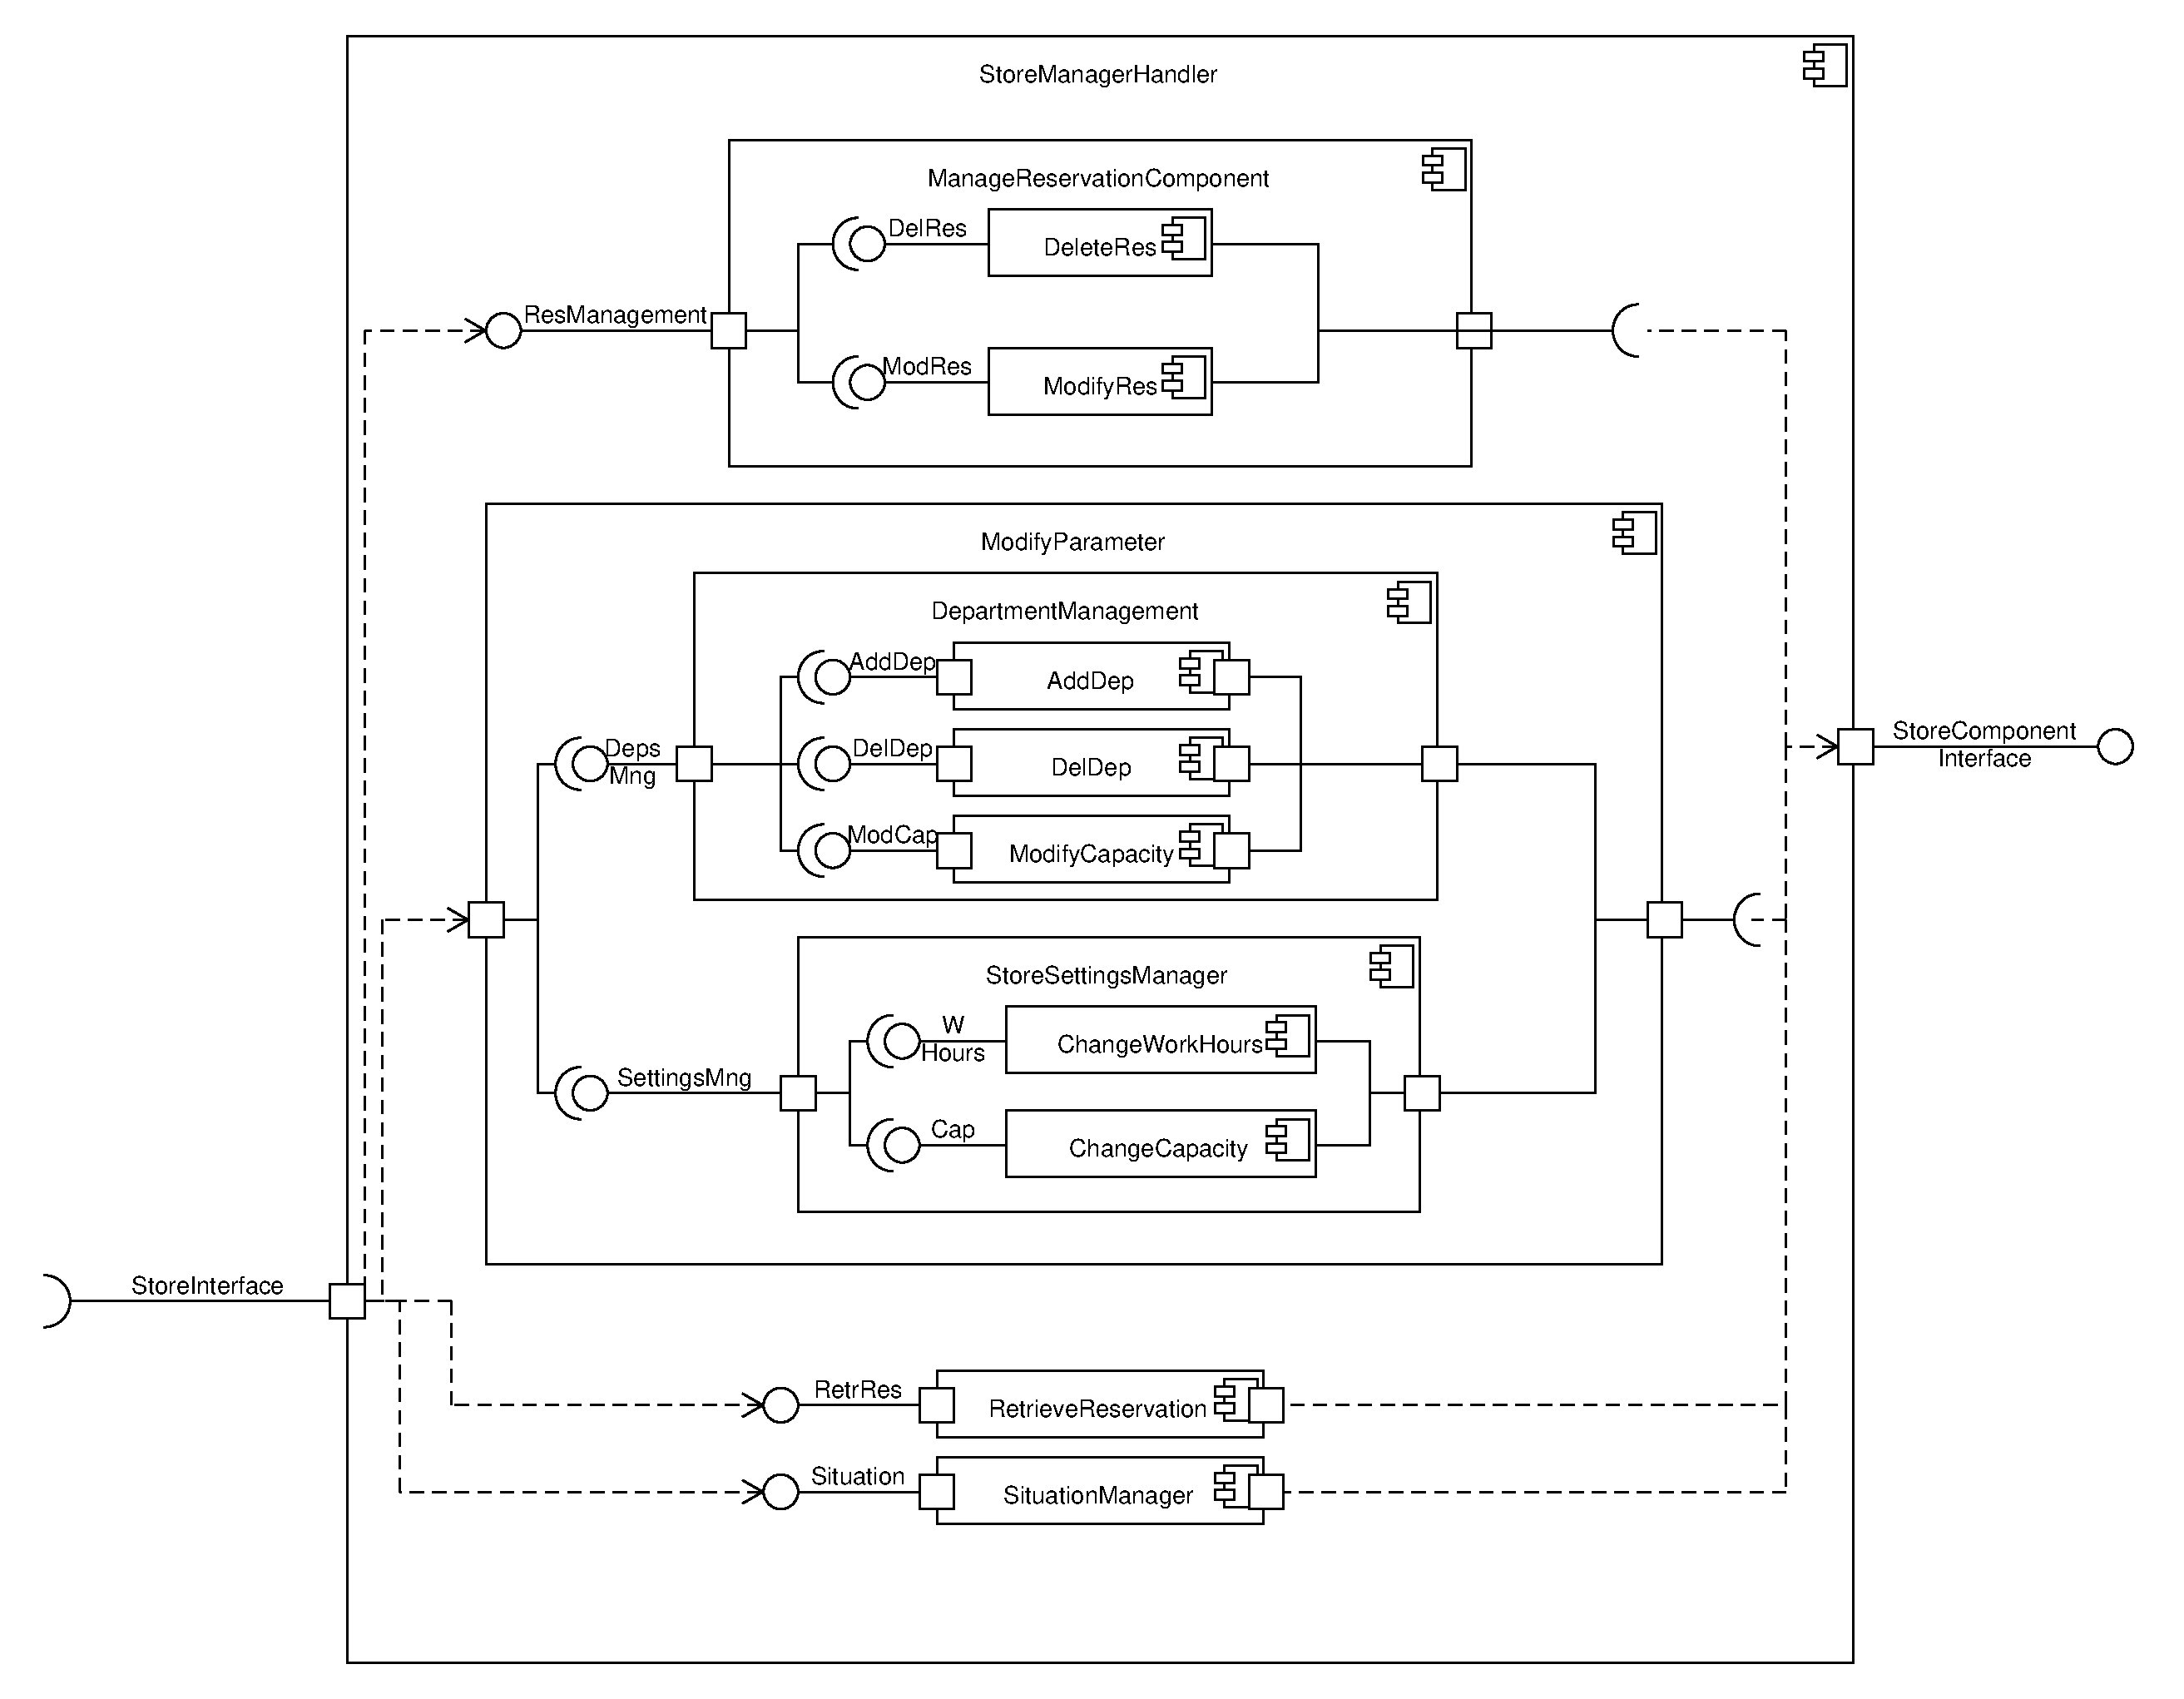
\includegraphics[scale=0.45]{Component Diagrams/StoreManagerHandlerComponentView.pdf}\\
			\end{adjustwidth}
			\caption{\emph{Store Manager Handler Component View}}
		\end{figure}
		\newpage
	\subsection{Deployment View}
	\subsection{Runtime View}
	\subsection{Component Interfaces}
	\subsection{Selected Architectural Styles and Patterns}
	\subsection{Other design decisions}

\section{User Interface Design}
This section shows and describes accurately the mockups of the application, in order to explain how the main functionalities will be offered. The first subsection is dedicated to the illustration of the application flow, shown using two different UX diagram, one for the customer and one for the store manager.

	\subsection{UX Diagrams}
	The following figures shows the application flow from the customer and the store manager point of view.
	
		\subsubsection{Customer Flow}
				\begin{figure}[H]
			\begin{adjustwidth} {-4cm}{}
				\centering
				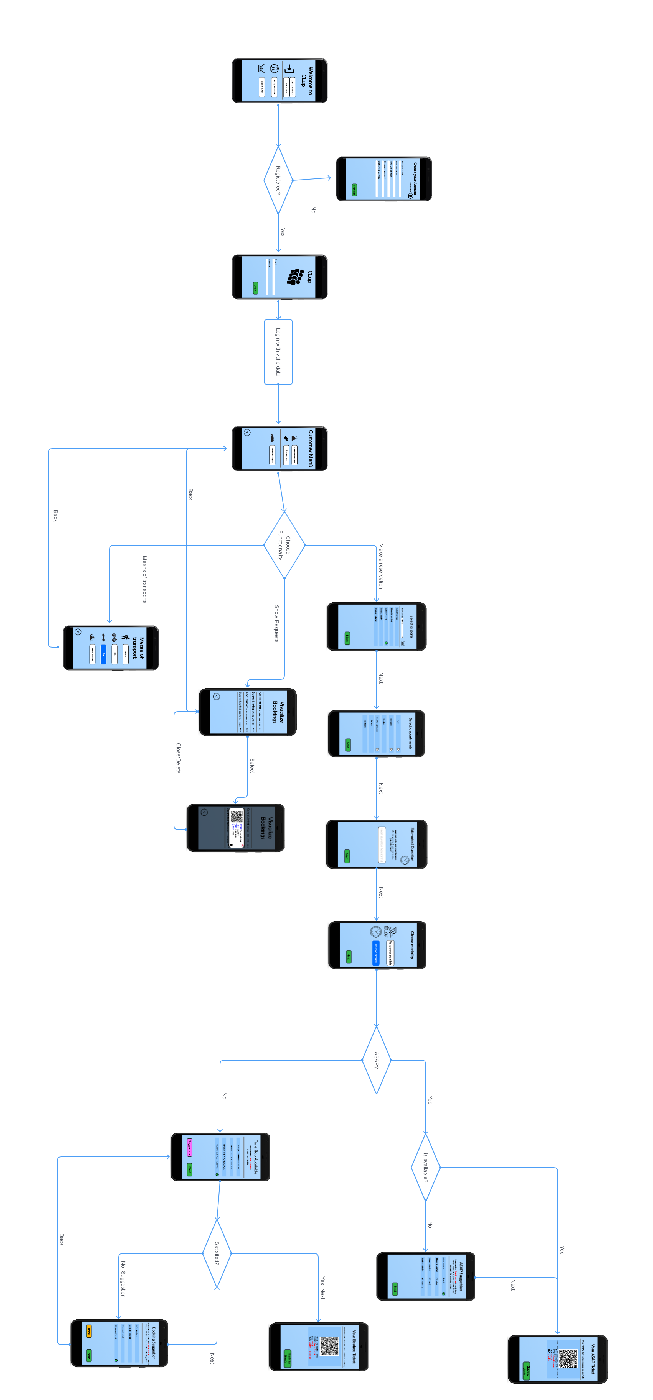
\includegraphics[scale=0.45]{../Mockups/UXDiagrams/CustomerFlow.pdf}\\
			\end{adjustwidth}
			\caption{\emph{Customer Flow}}
		\end{figure}
	
		\subsubsection{Store Manager Flow}
		...

	\subsection{Customer POV}
		\subsubsection{Registration and Login}
		the mockup in Figure ??? is the initial page every user will see the first time he uses CLup. A user can interact with the system only if authenticated (as customer or store manager); therefore each first-time user will choose one of the sign up buttons for registering.
		
		Clicking on "Sign up as customer" will bring us to Figure ???, in which a new (unregistered) customer has to enter his data (Email, name, surname and a password) and click "Sign up" in order to create the account.
		
		Clicking on "Login as customer" will bring us to Figure ???, in which a customer can enter his Email and password in order to log in.
		
		After the login we will be on Figure ???
		
		\begin{figure}[H]
			\begin{adjustwidth} {-4cm}{}
				\centering
				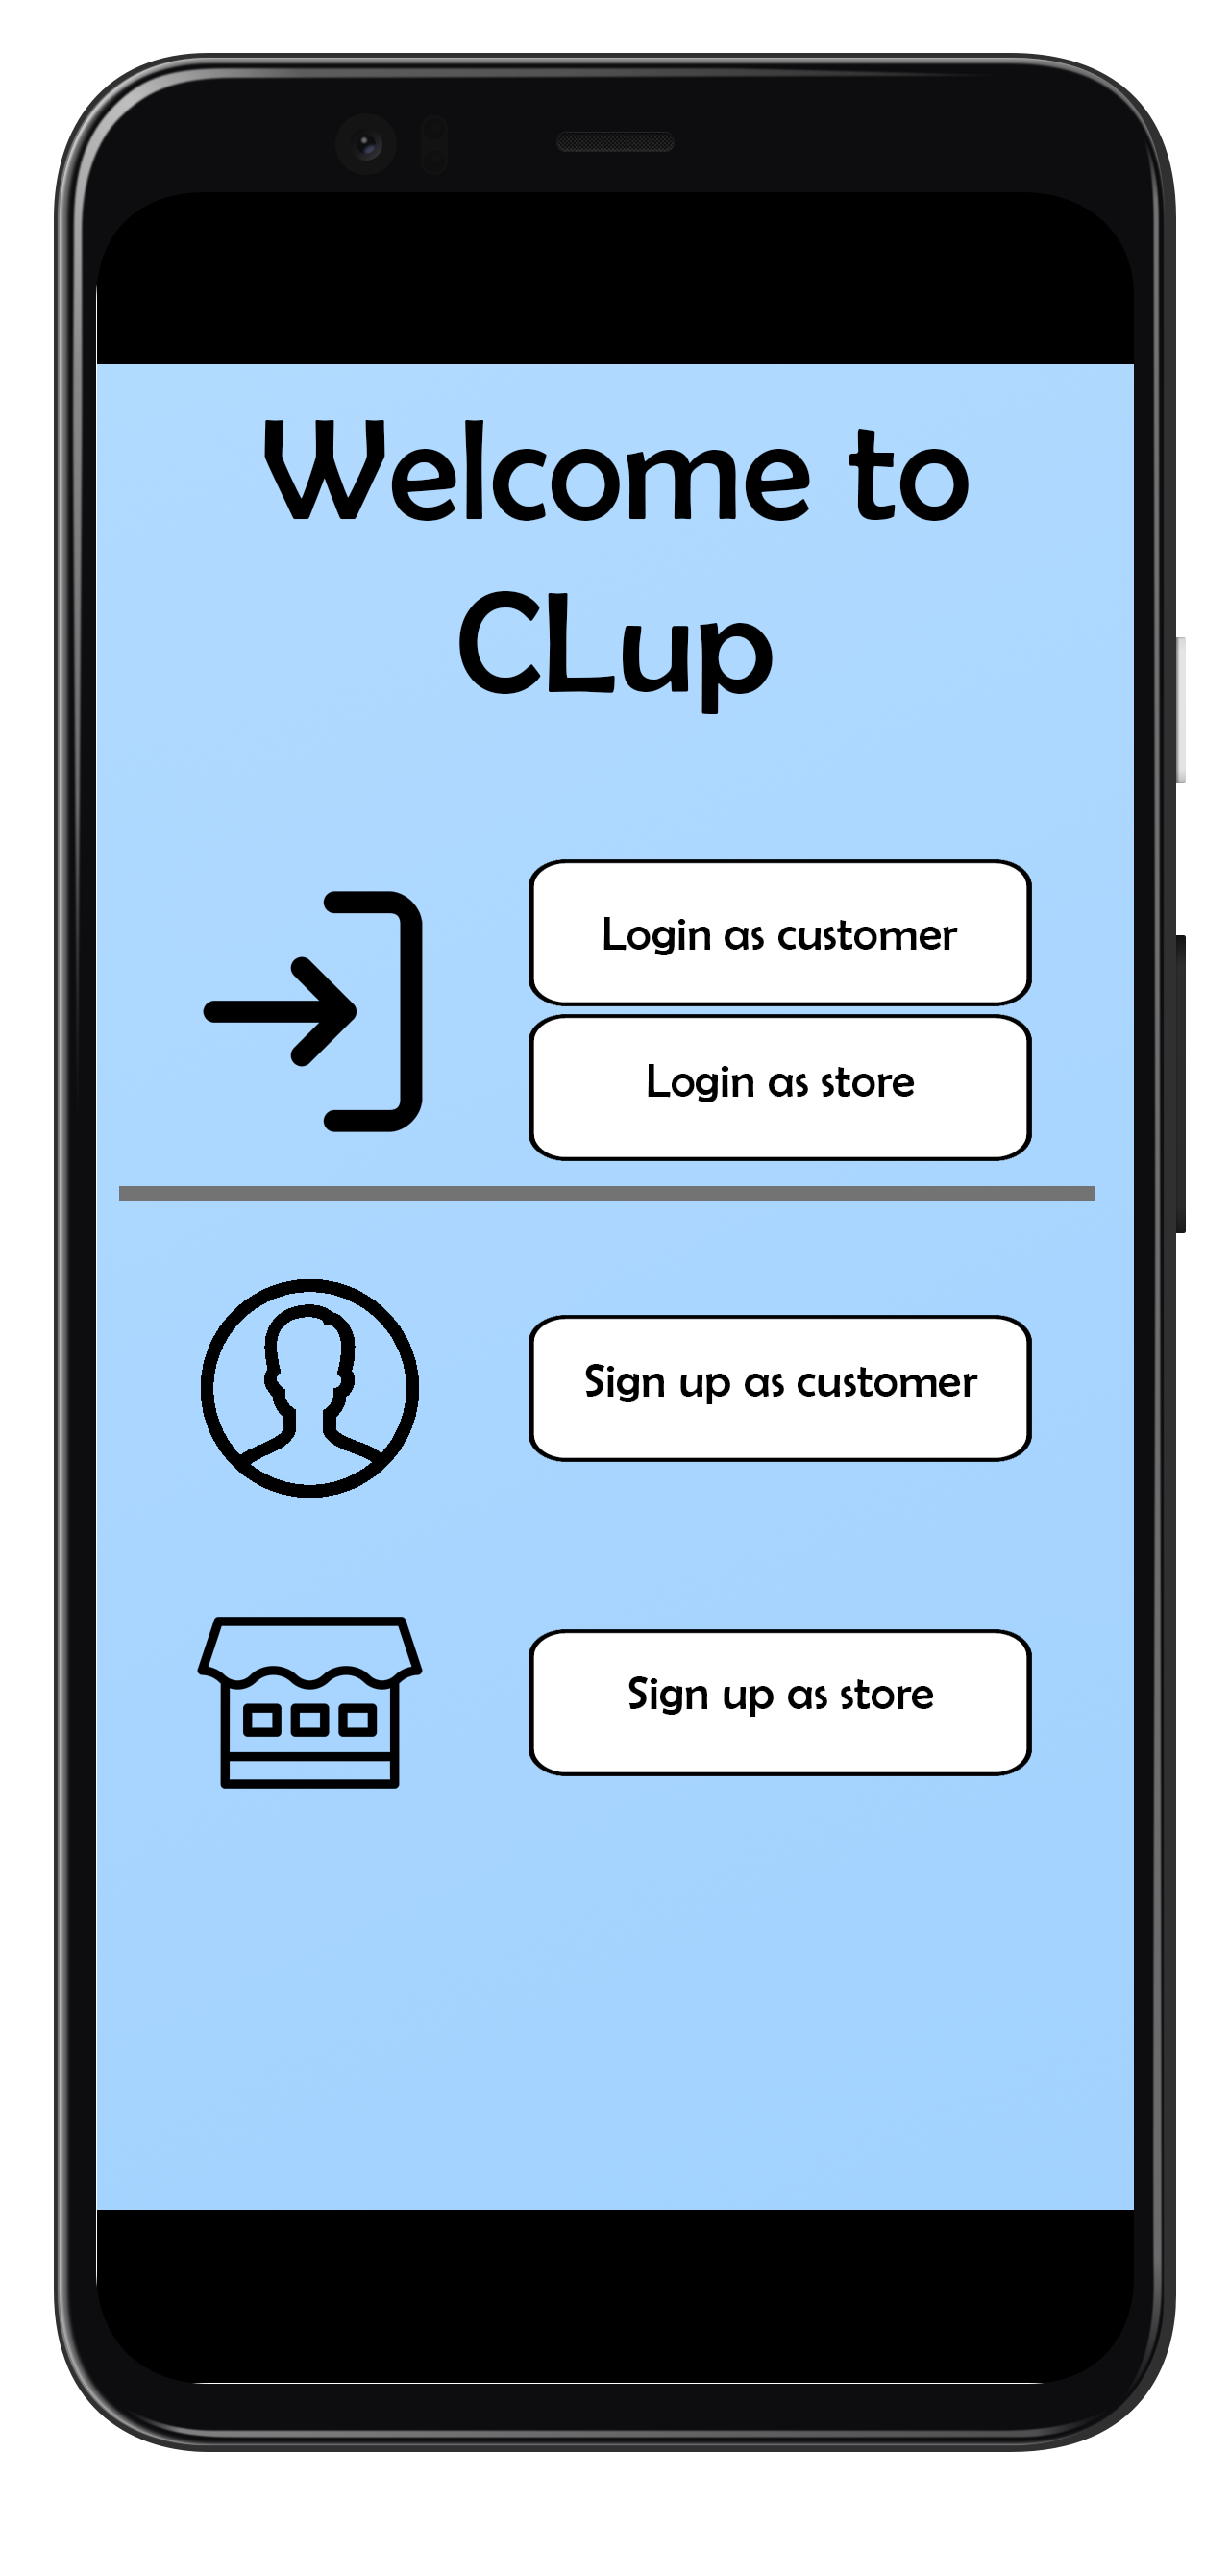
\includegraphics[scale=0.45]{../Mockups/InitialPage.png}\\
			\end{adjustwidth}
			\caption{\emph{Initial page}}
		\end{figure}
	
		\begin{figure}[H]
			\begin{adjustwidth} {-4cm}{}
				\centering
				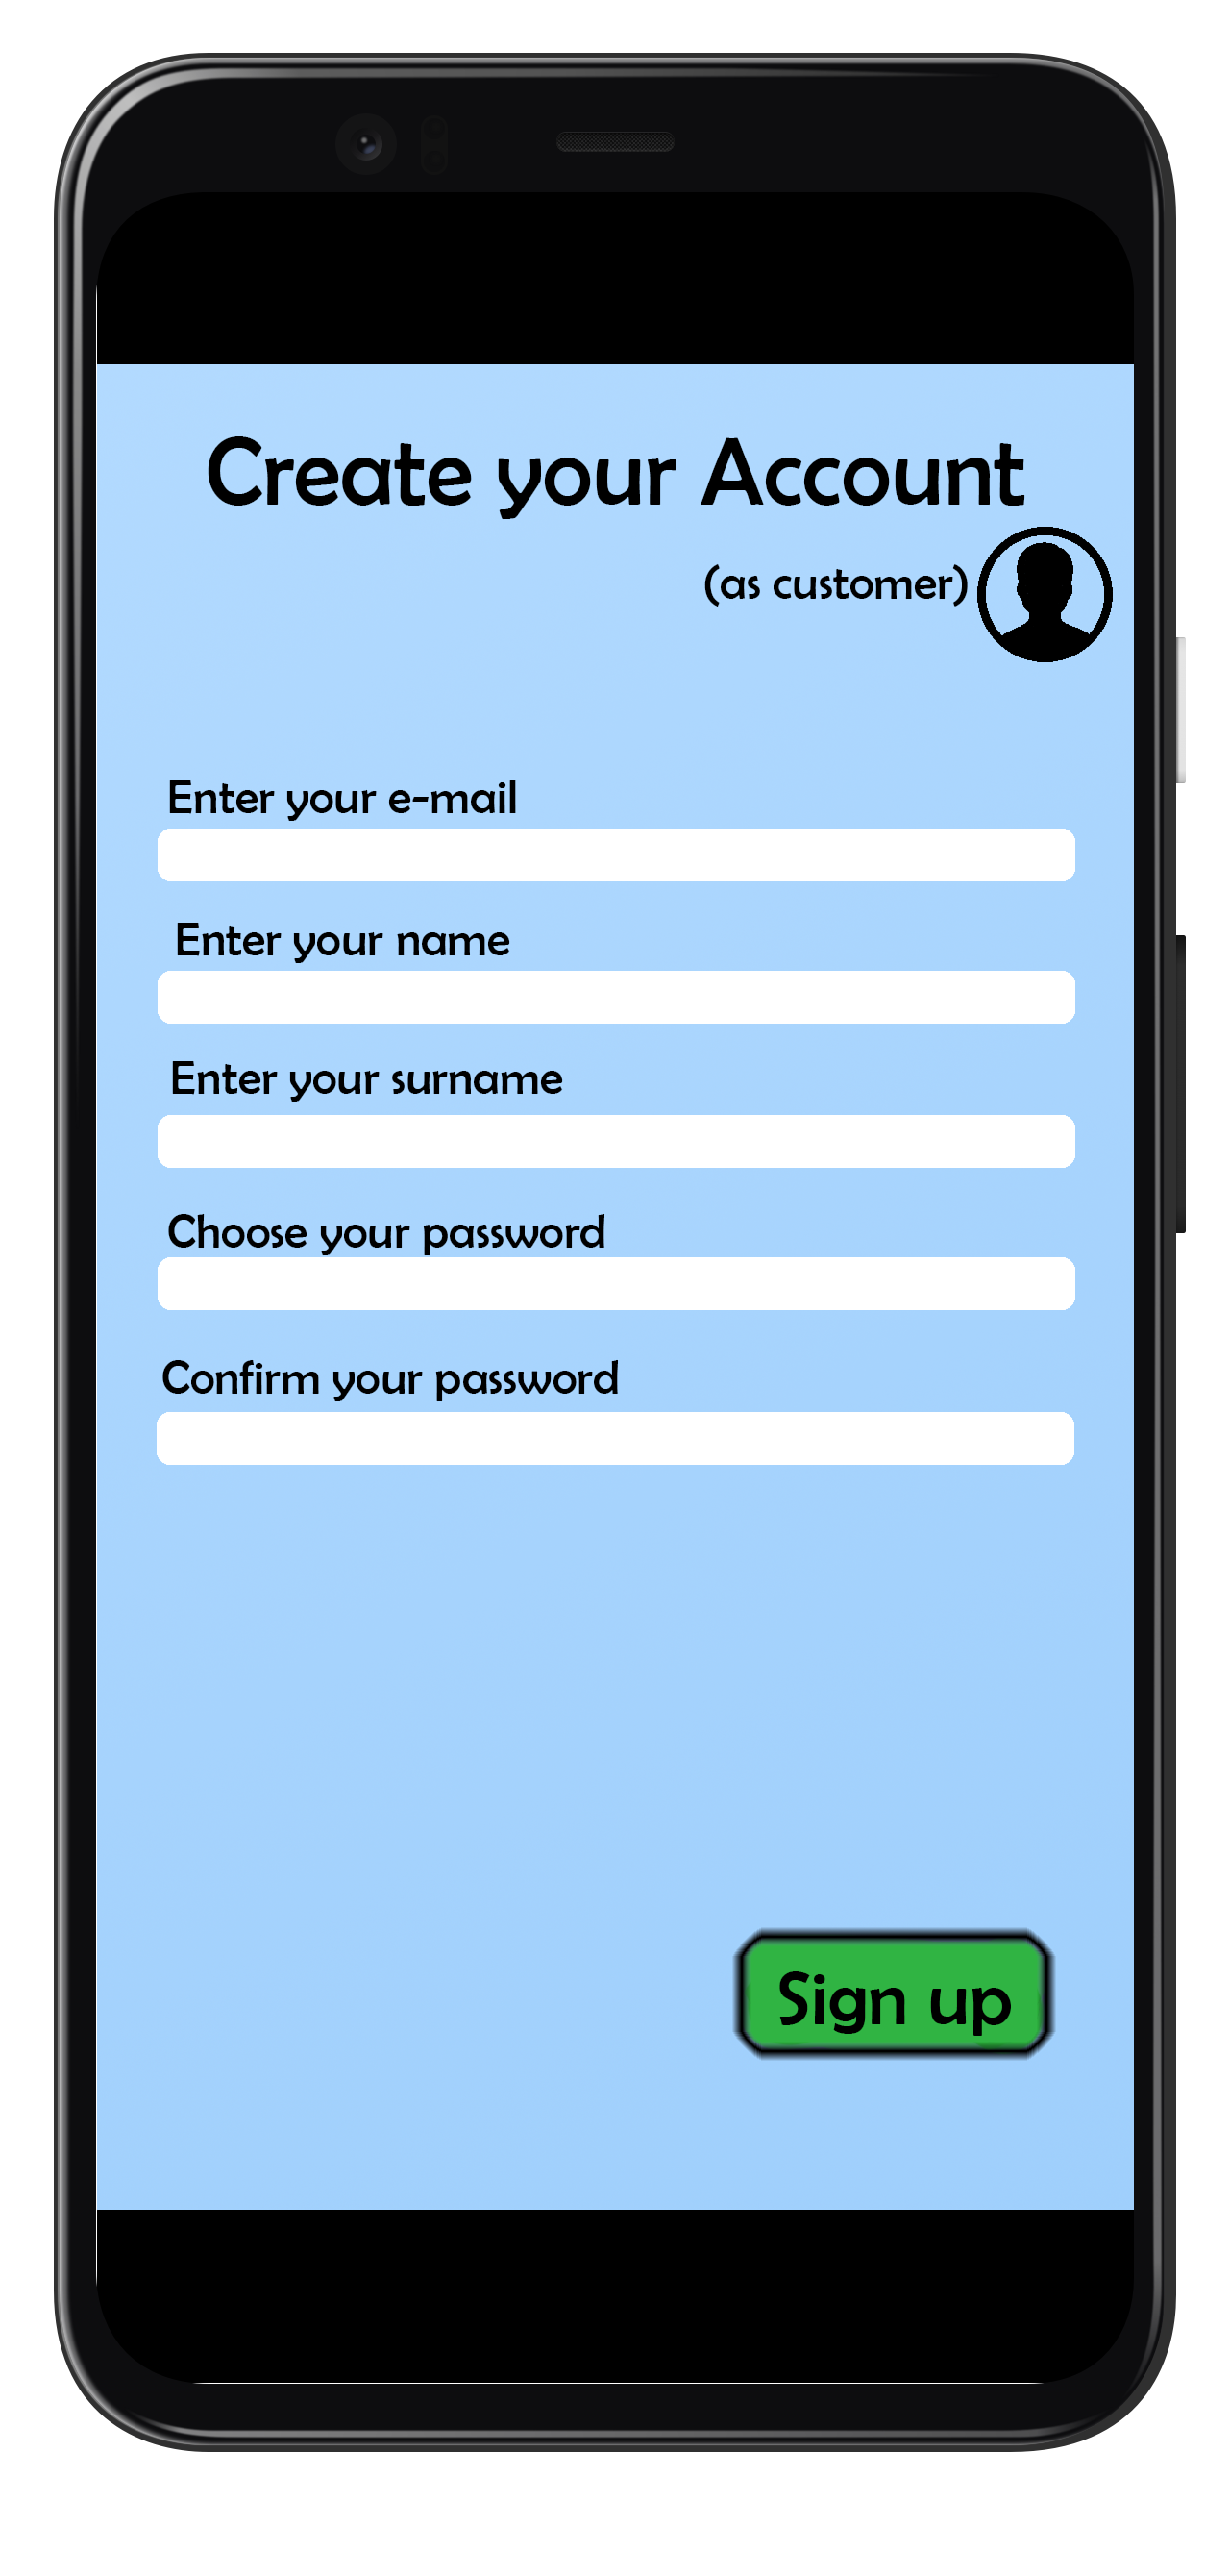
\includegraphics[scale=0.45]{../Mockups/SignUpCustomer.png}\\
			\end{adjustwidth}
			\caption{\emph{Sign up as customer}}
		\end{figure}
	
		\begin{figure}[H]
			\begin{adjustwidth} {-4cm}{}
				\centering
				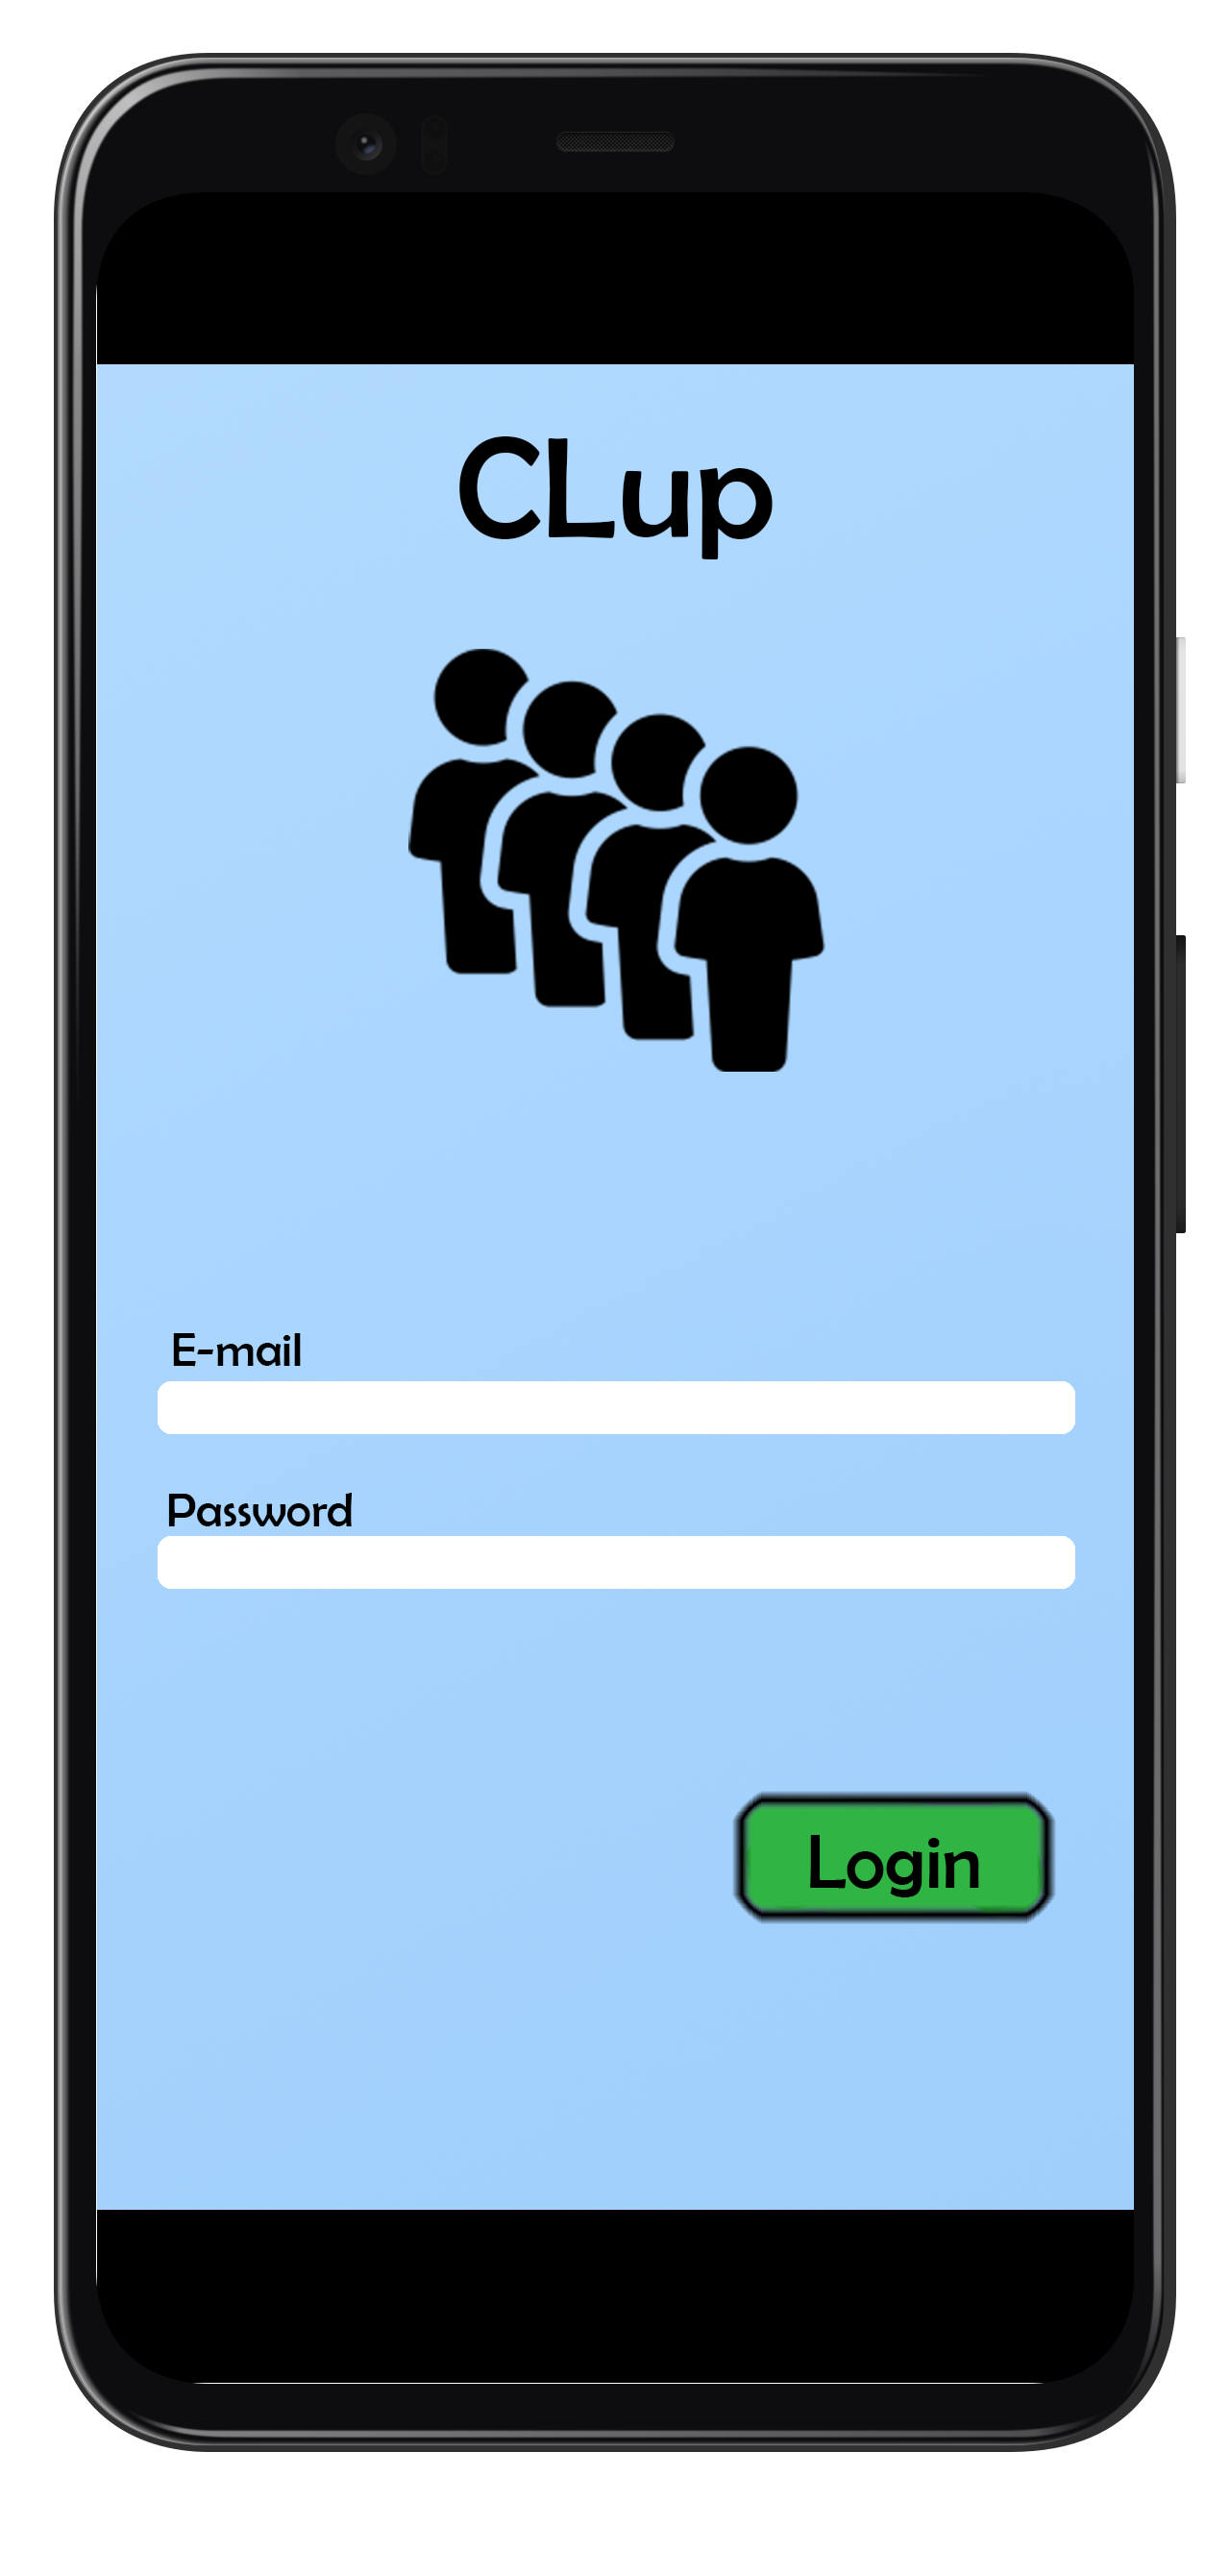
\includegraphics[scale=0.45]{../Mockups/LoginCustomer.png}\\
			\end{adjustwidth}
			\caption{\emph{Login as customer}}
		\end{figure}
		
		
		
		\subsubsection{Make a reservation}
		
		Clicking on "Make a reservation" will bring us to Figure ???, where we have to select the store we want to go to, then in Figure ??? we can select the departments that we want to visit, in Figure ?? we can indicate the estimated time of our grocery, and in Figure ??? we can choose the reservation modality: ASAP or at a specific date and time.
		
		\begin{figure}[H]
			\begin{adjustwidth} {-4cm}{}
				\centering
				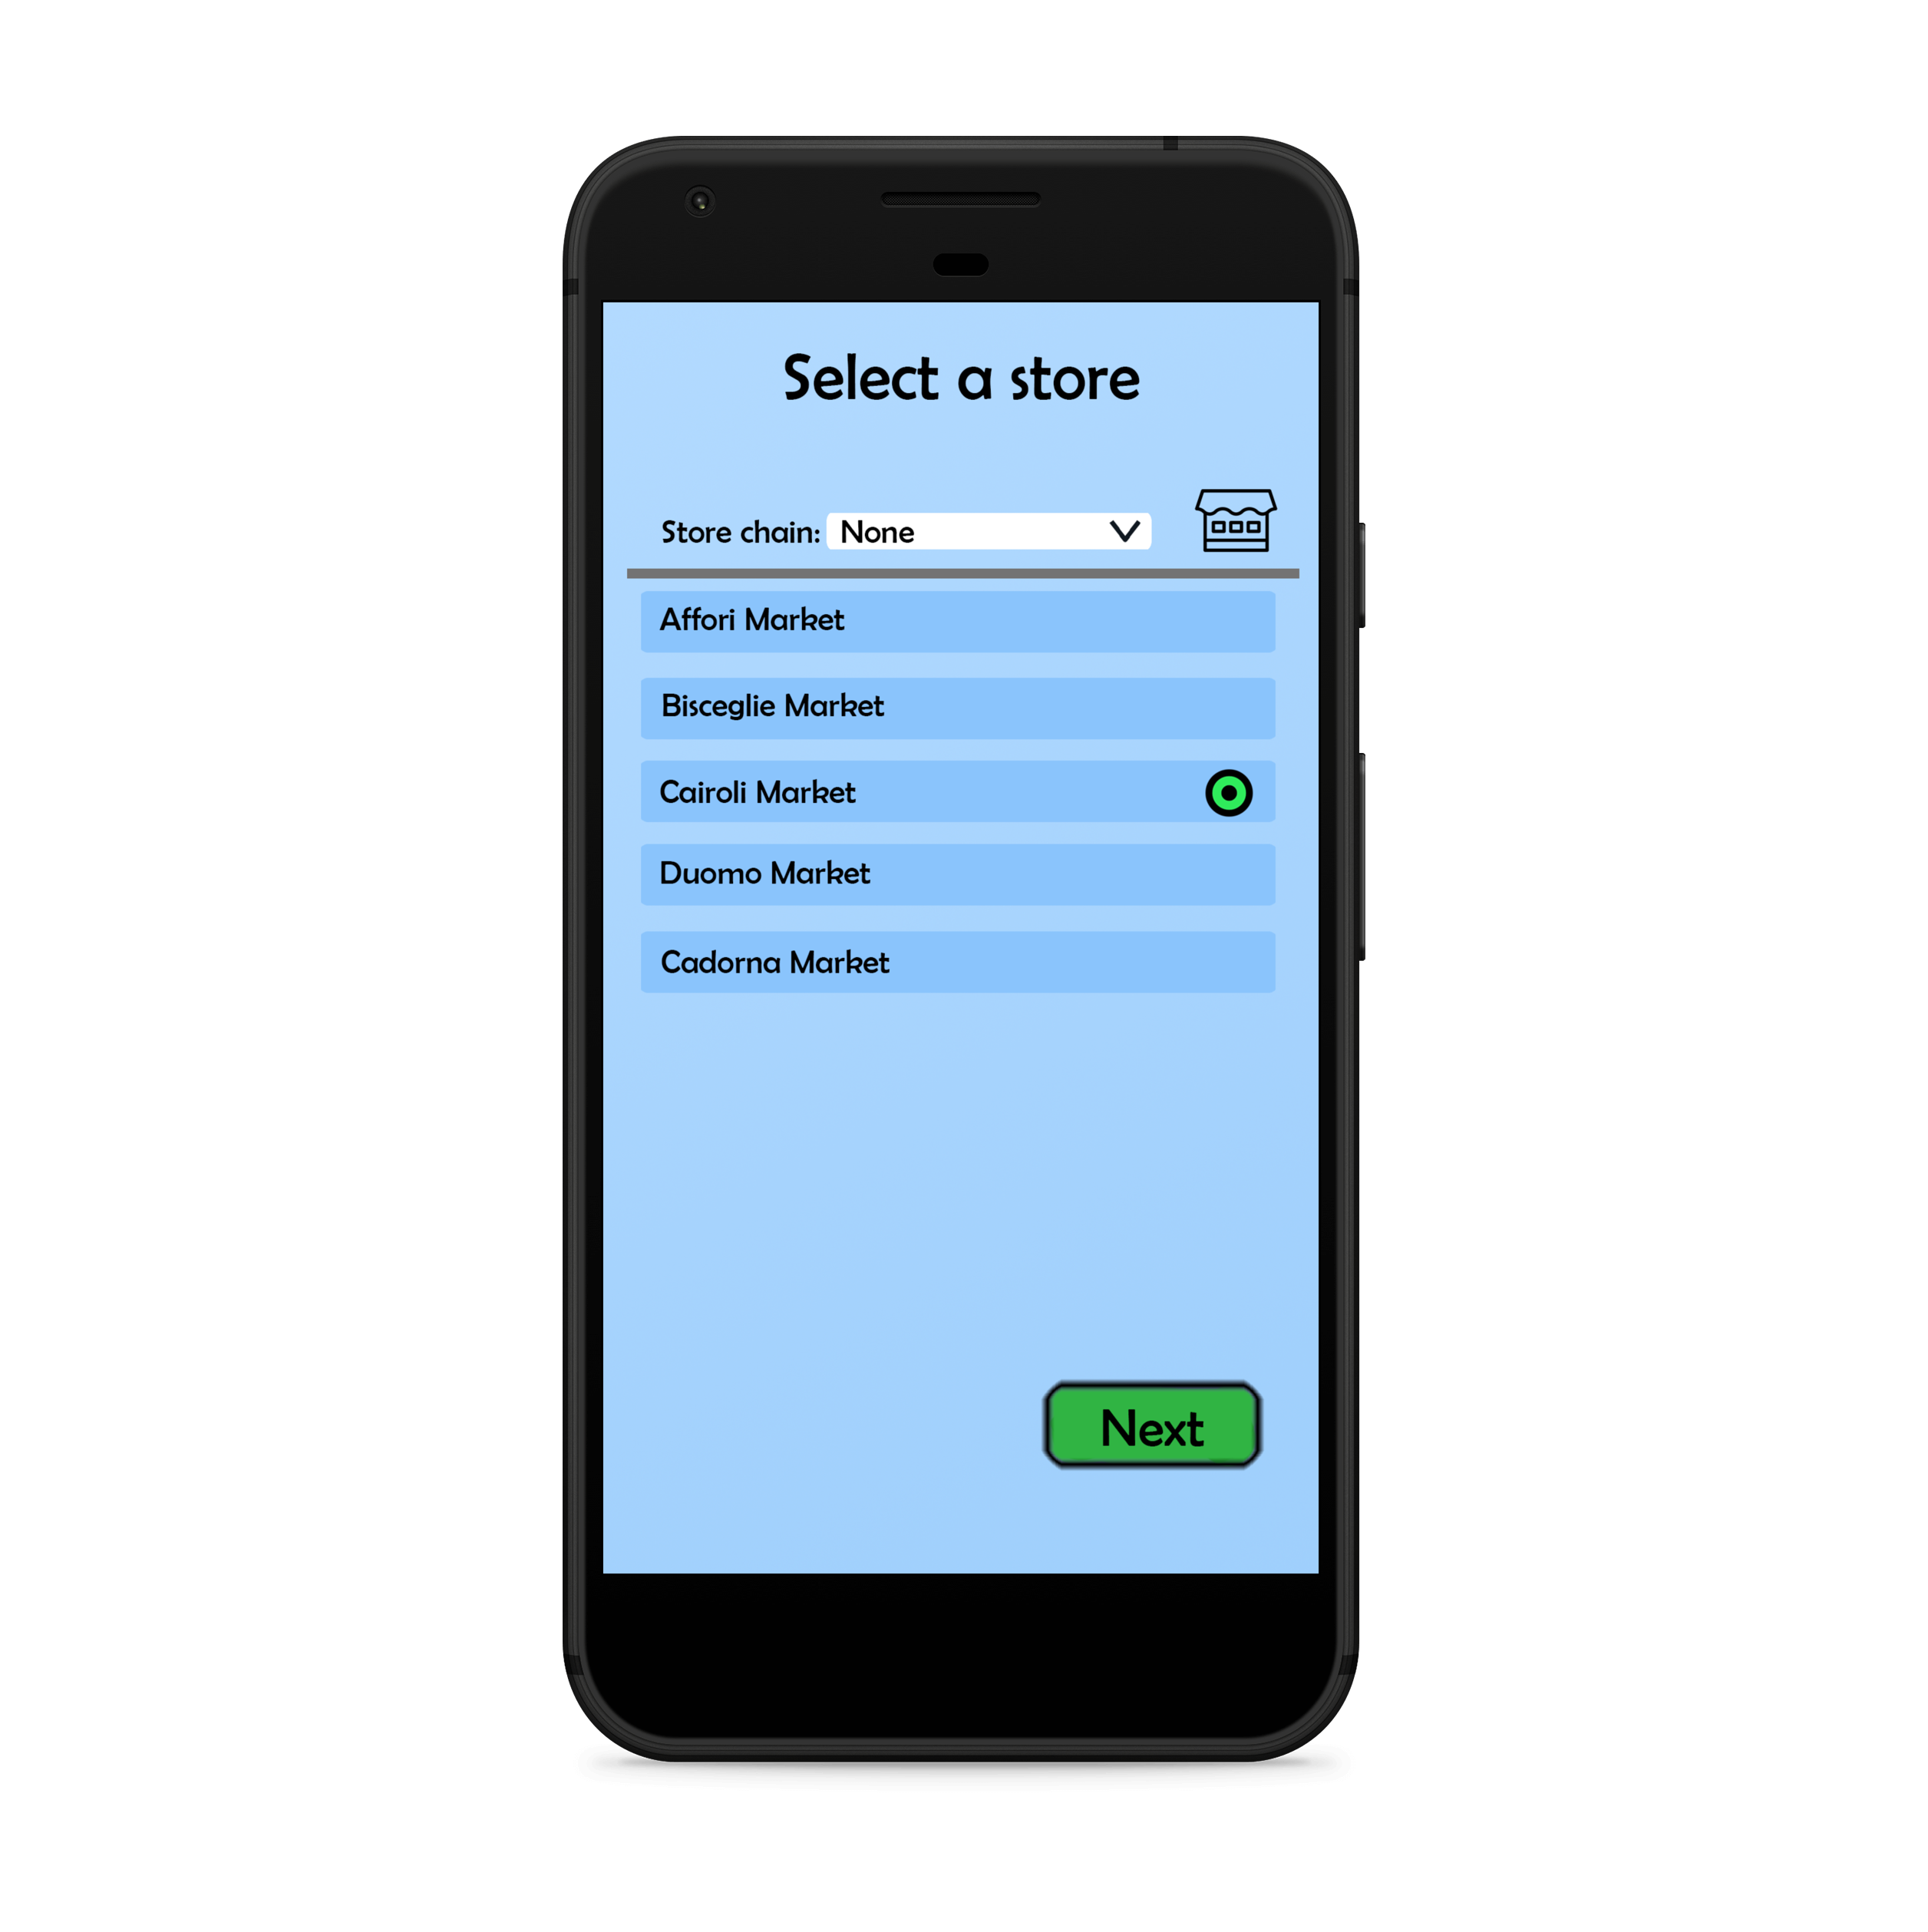
\includegraphics[scale=0.45]{../Mockups/SelectStore.png}\\
			\end{adjustwidth}
			\caption{\emph{Store selection}}
		\end{figure}
	
		\begin{figure}[H]
		\begin{adjustwidth} {-4cm}{}
			\centering
			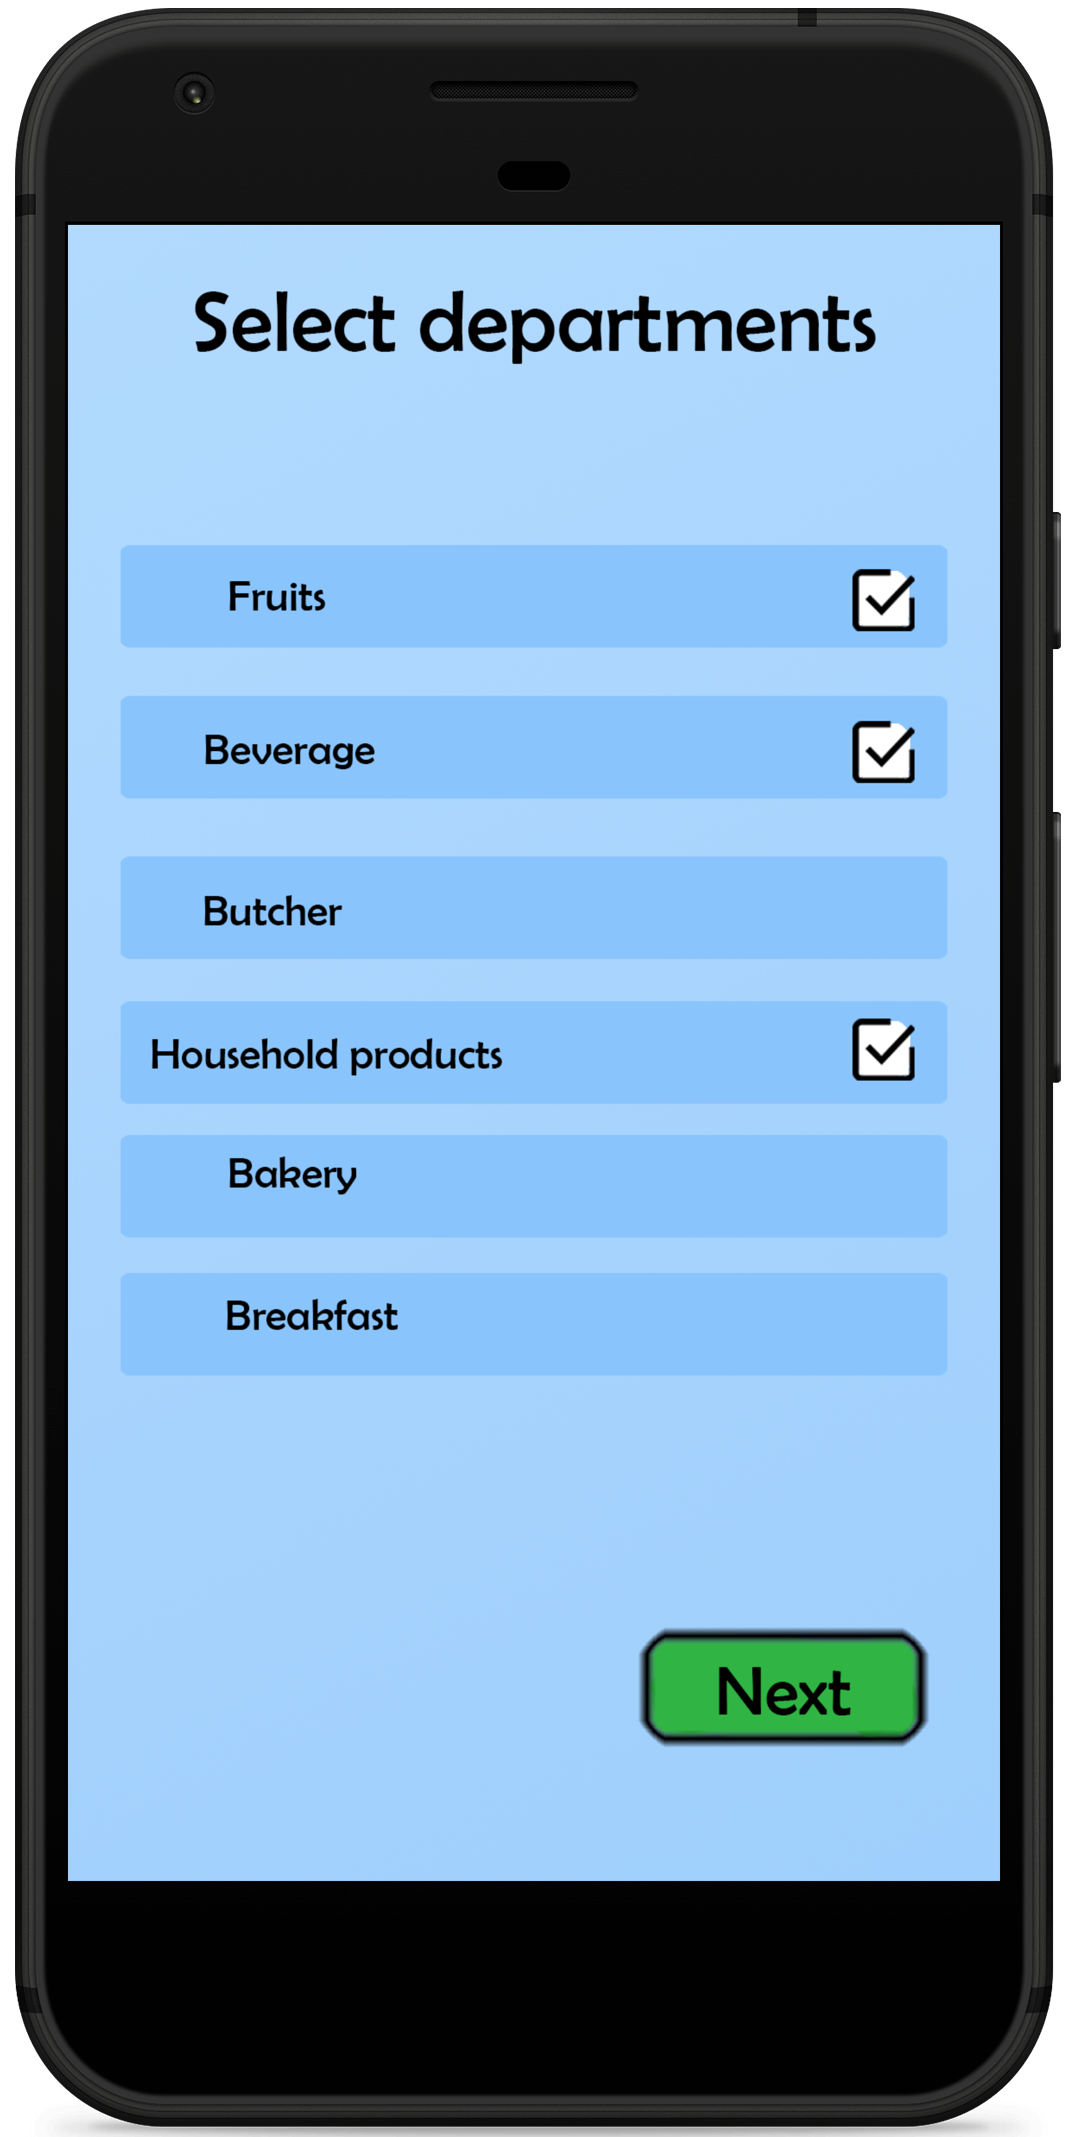
\includegraphics[scale=0.45]{../Mockups/SelectDepartments.png}\\
		\end{adjustwidth}
		\caption{\emph{Departments selection}}
		\end{figure}
	
		\begin{figure}[H]
			\begin{adjustwidth} {-4cm}{}
				\centering
				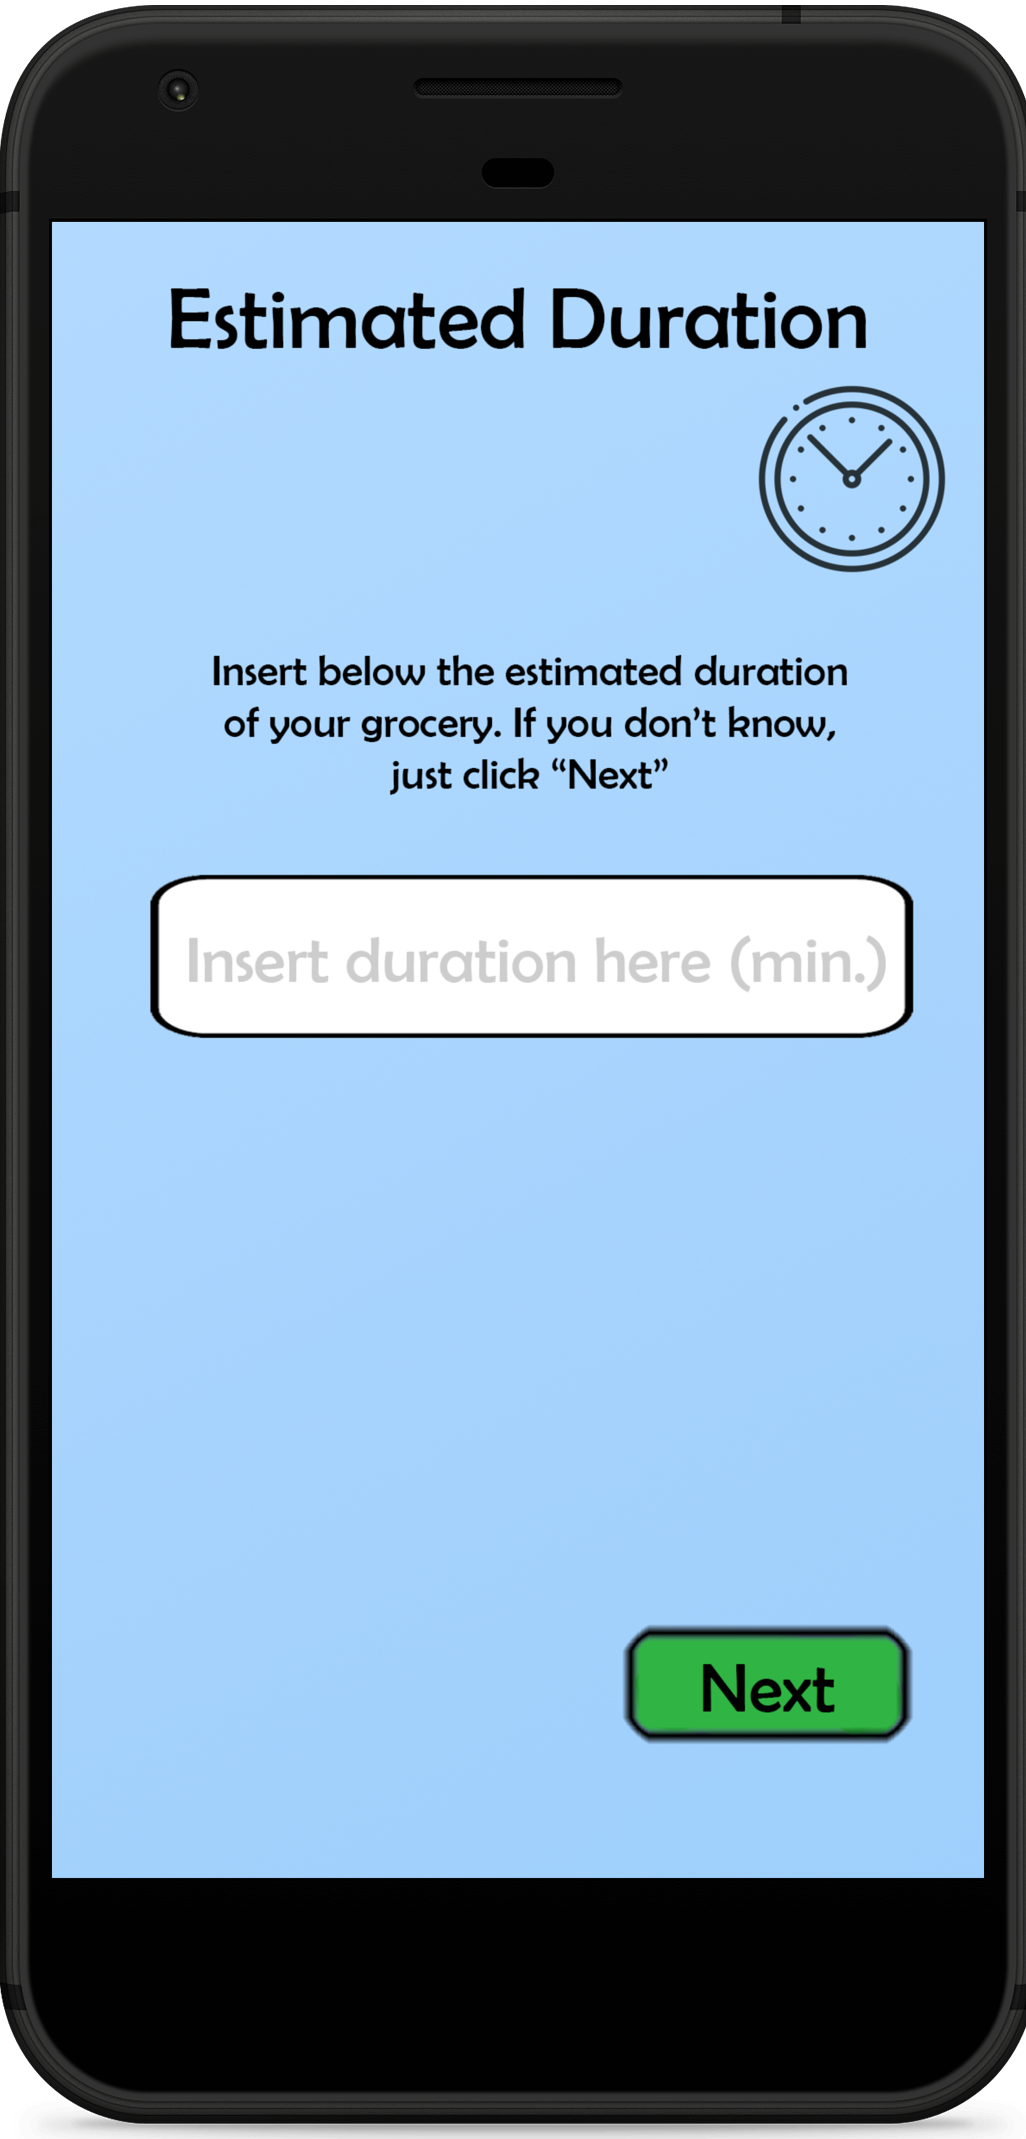
\includegraphics[scale=0.45]{../Mockups/EstimatedDuration.png}\\
			\end{adjustwidth}
			\caption{\emph{Estimated duration}}
		\end{figure}
	
		\begin{figure}[H]
			\begin{adjustwidth} {-4cm}{}
				\centering
				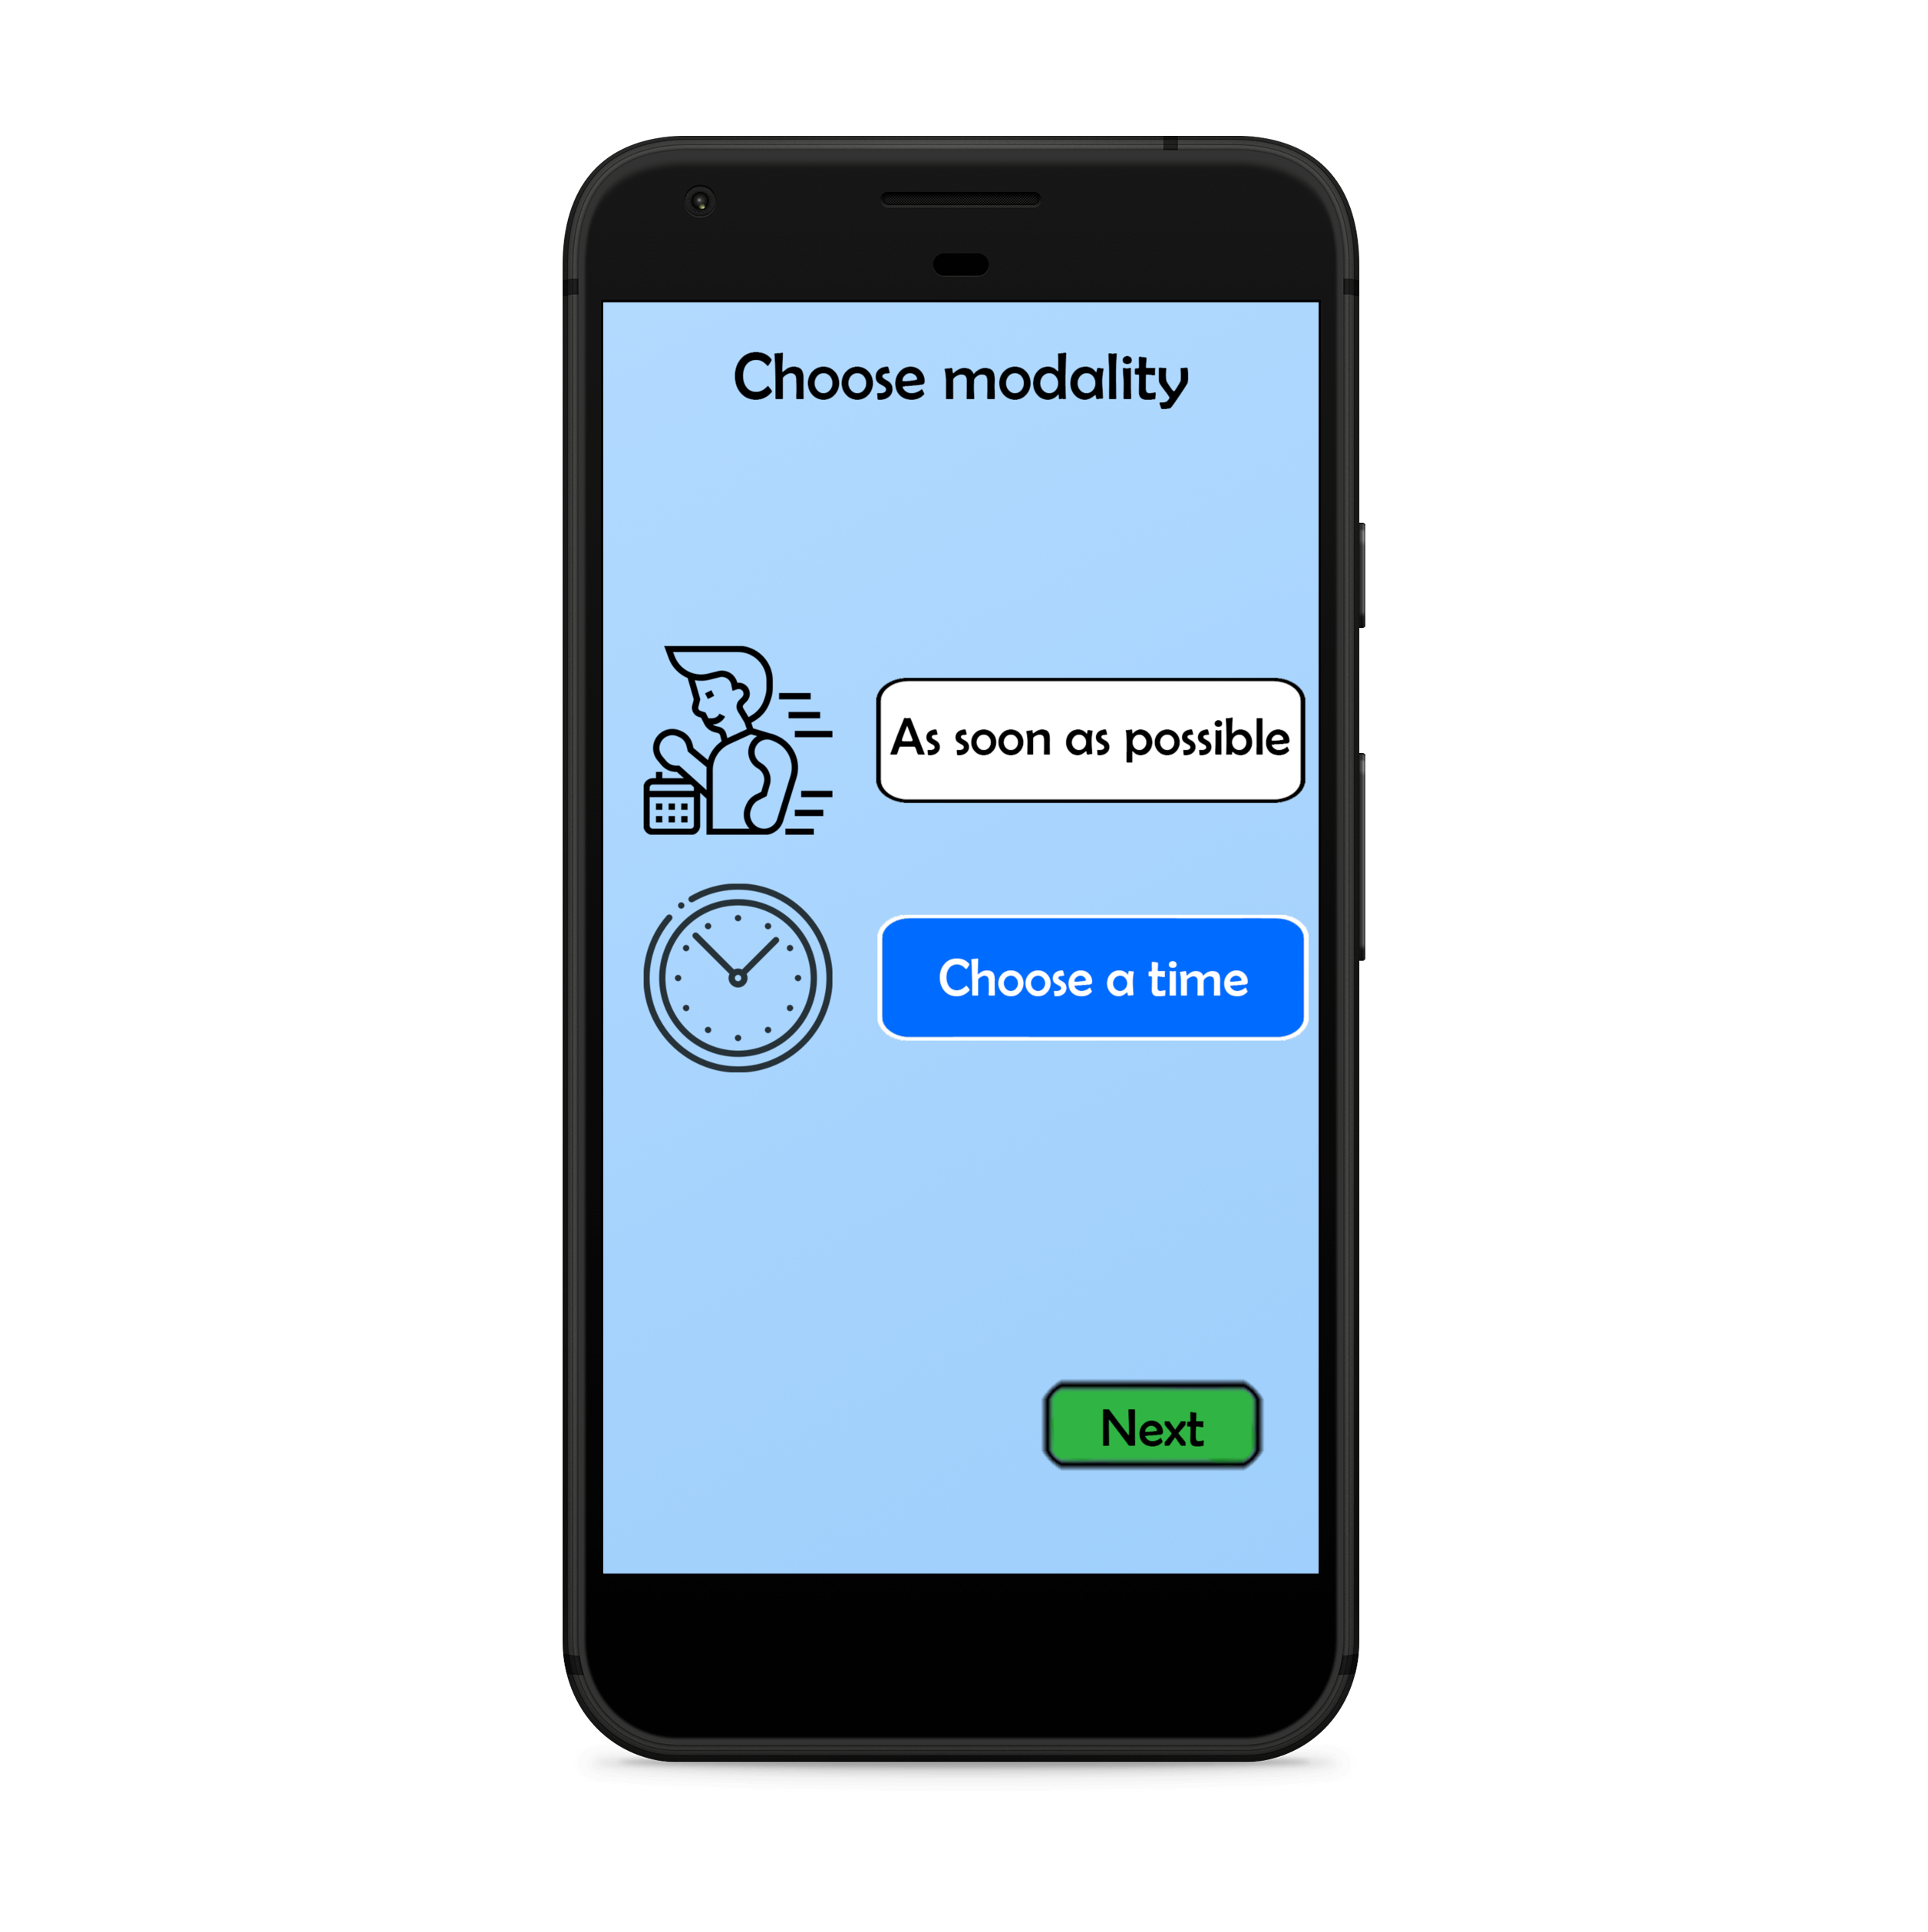
\includegraphics[scale=0.45]{../Mockups/ChooseModality.png}\\
			\end{adjustwidth}
			\caption{\emph{Choice of modality}}
		\end{figure}
		
		ASAP: choosing the ASAP modality can bring us to Figure ??? if the system find a suitable time slot, or to Figure ??? if there is no suitable time slot for the selected store; in the latter case, we can choose another store where is possible to do an ASAP reservation.
		
		\begin{figure}[H]
			\begin{adjustwidth} {-4cm}{}
				\centering
				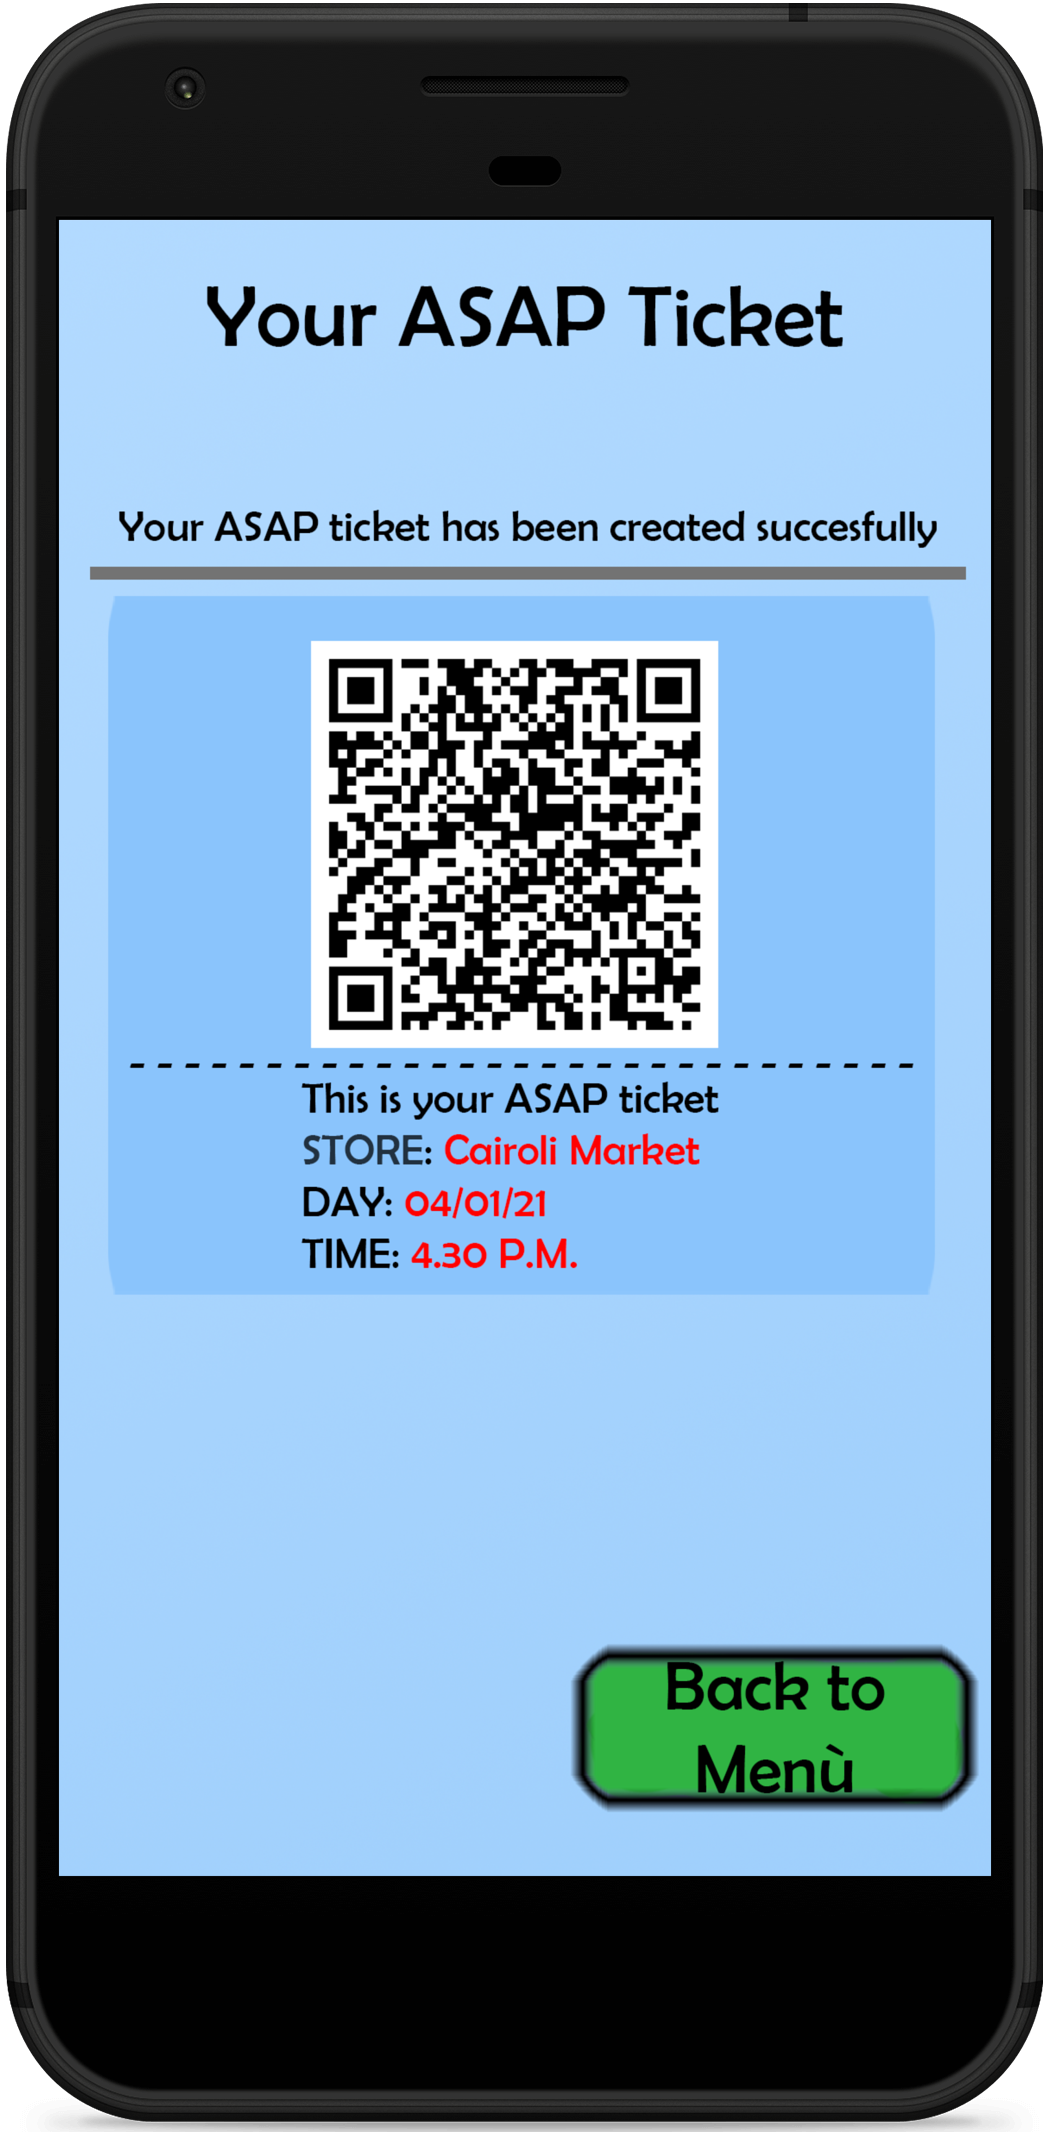
\includegraphics[scale=0.45]{../Mockups/ASAPTicket.png}\\
			\end{adjustwidth}
			\caption{\emph{Creation of ASAP ticket}}
		\end{figure}
	
		\begin{figure}[H]
			\begin{adjustwidth} {-4cm}{}
				\centering
				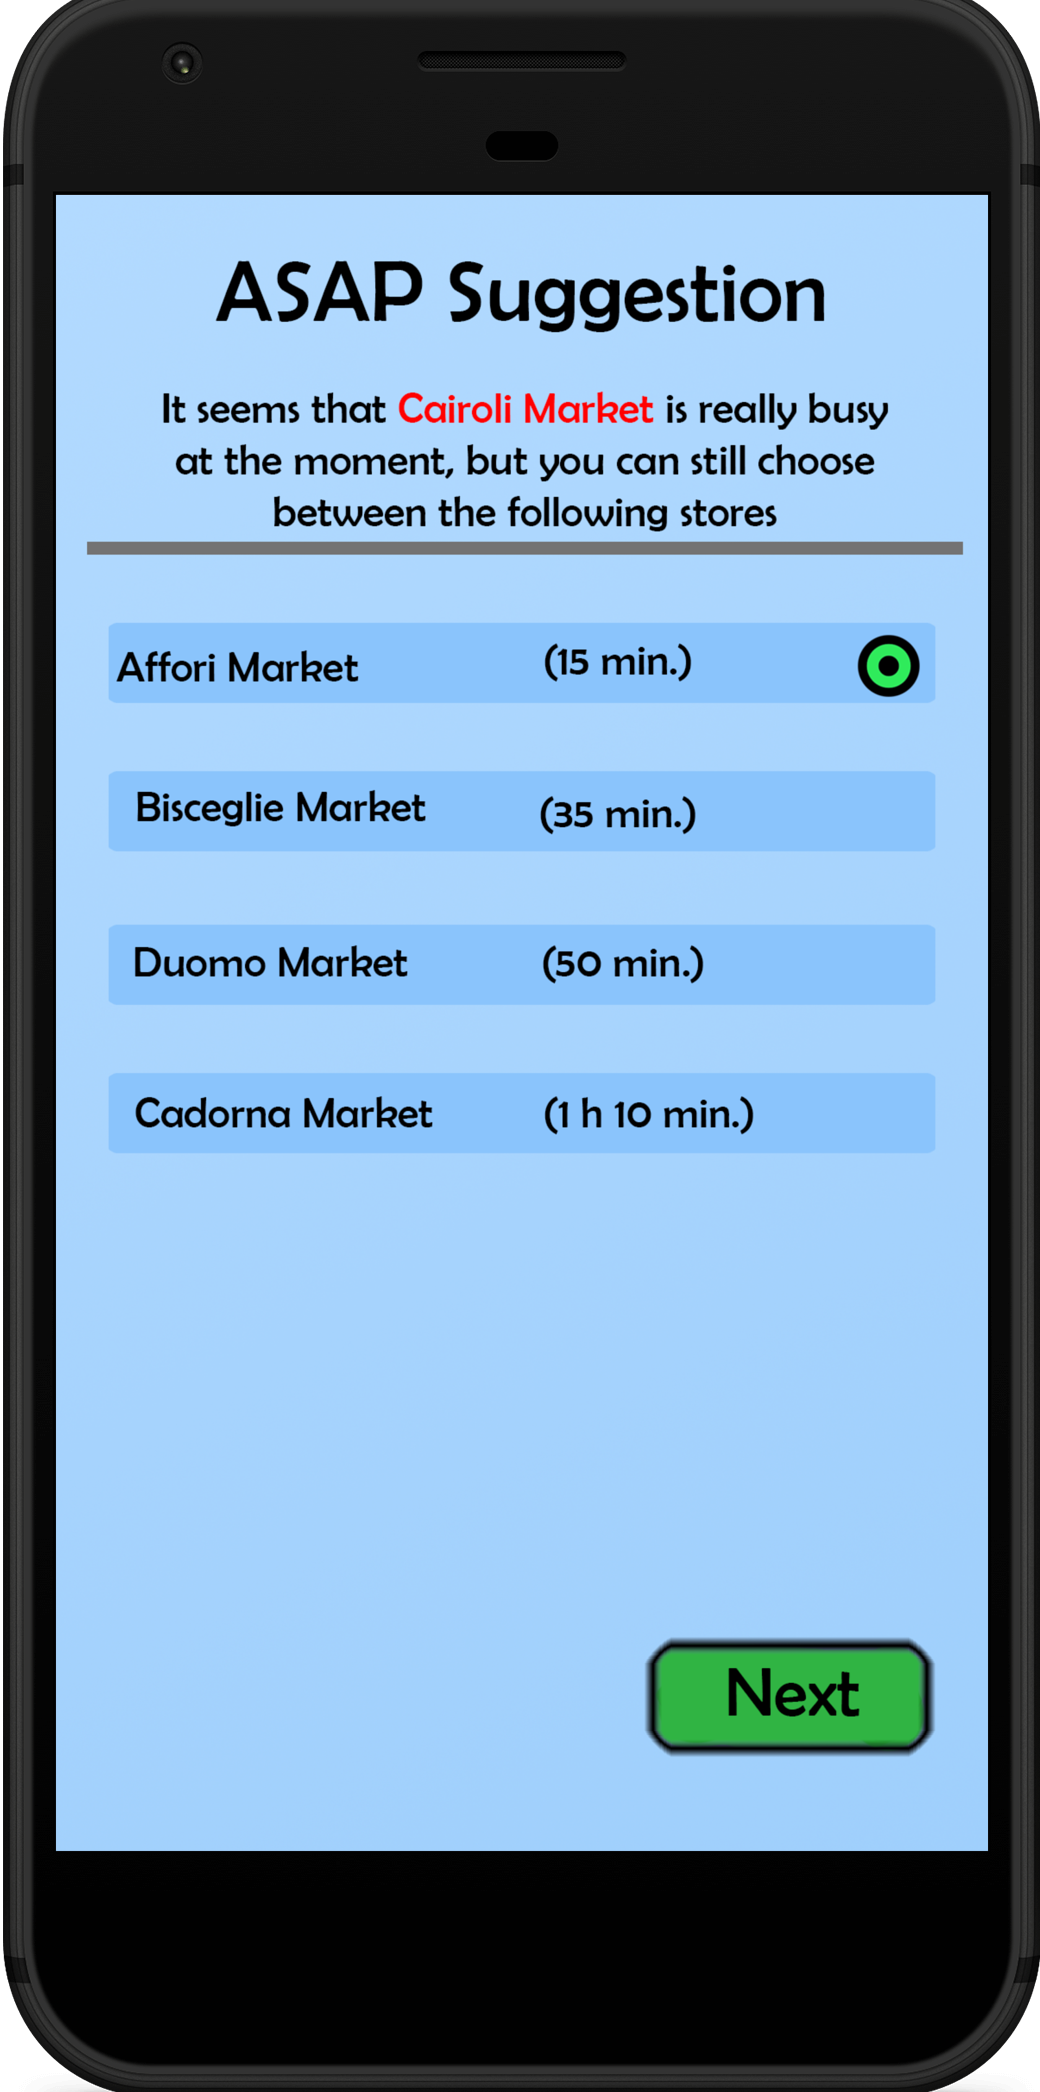
\includegraphics[scale=0.45]{../Mockups/ASAPSuggestion.png}\\
			\end{adjustwidth}
			\caption{\emph{ASAP suggestions}}
		\end{figure}
		
		Booking: choosing the booking modality will bring us to Figure ???; if we find a time slot that is good for us, we can select it and create the reservation (Figure ???), otherwise we can click "Suggestion" that will bring us to Figure ???, where the system show us other store.
		
		\begin{figure}[H]
			\begin{adjustwidth} {-4cm}{}
				\centering
				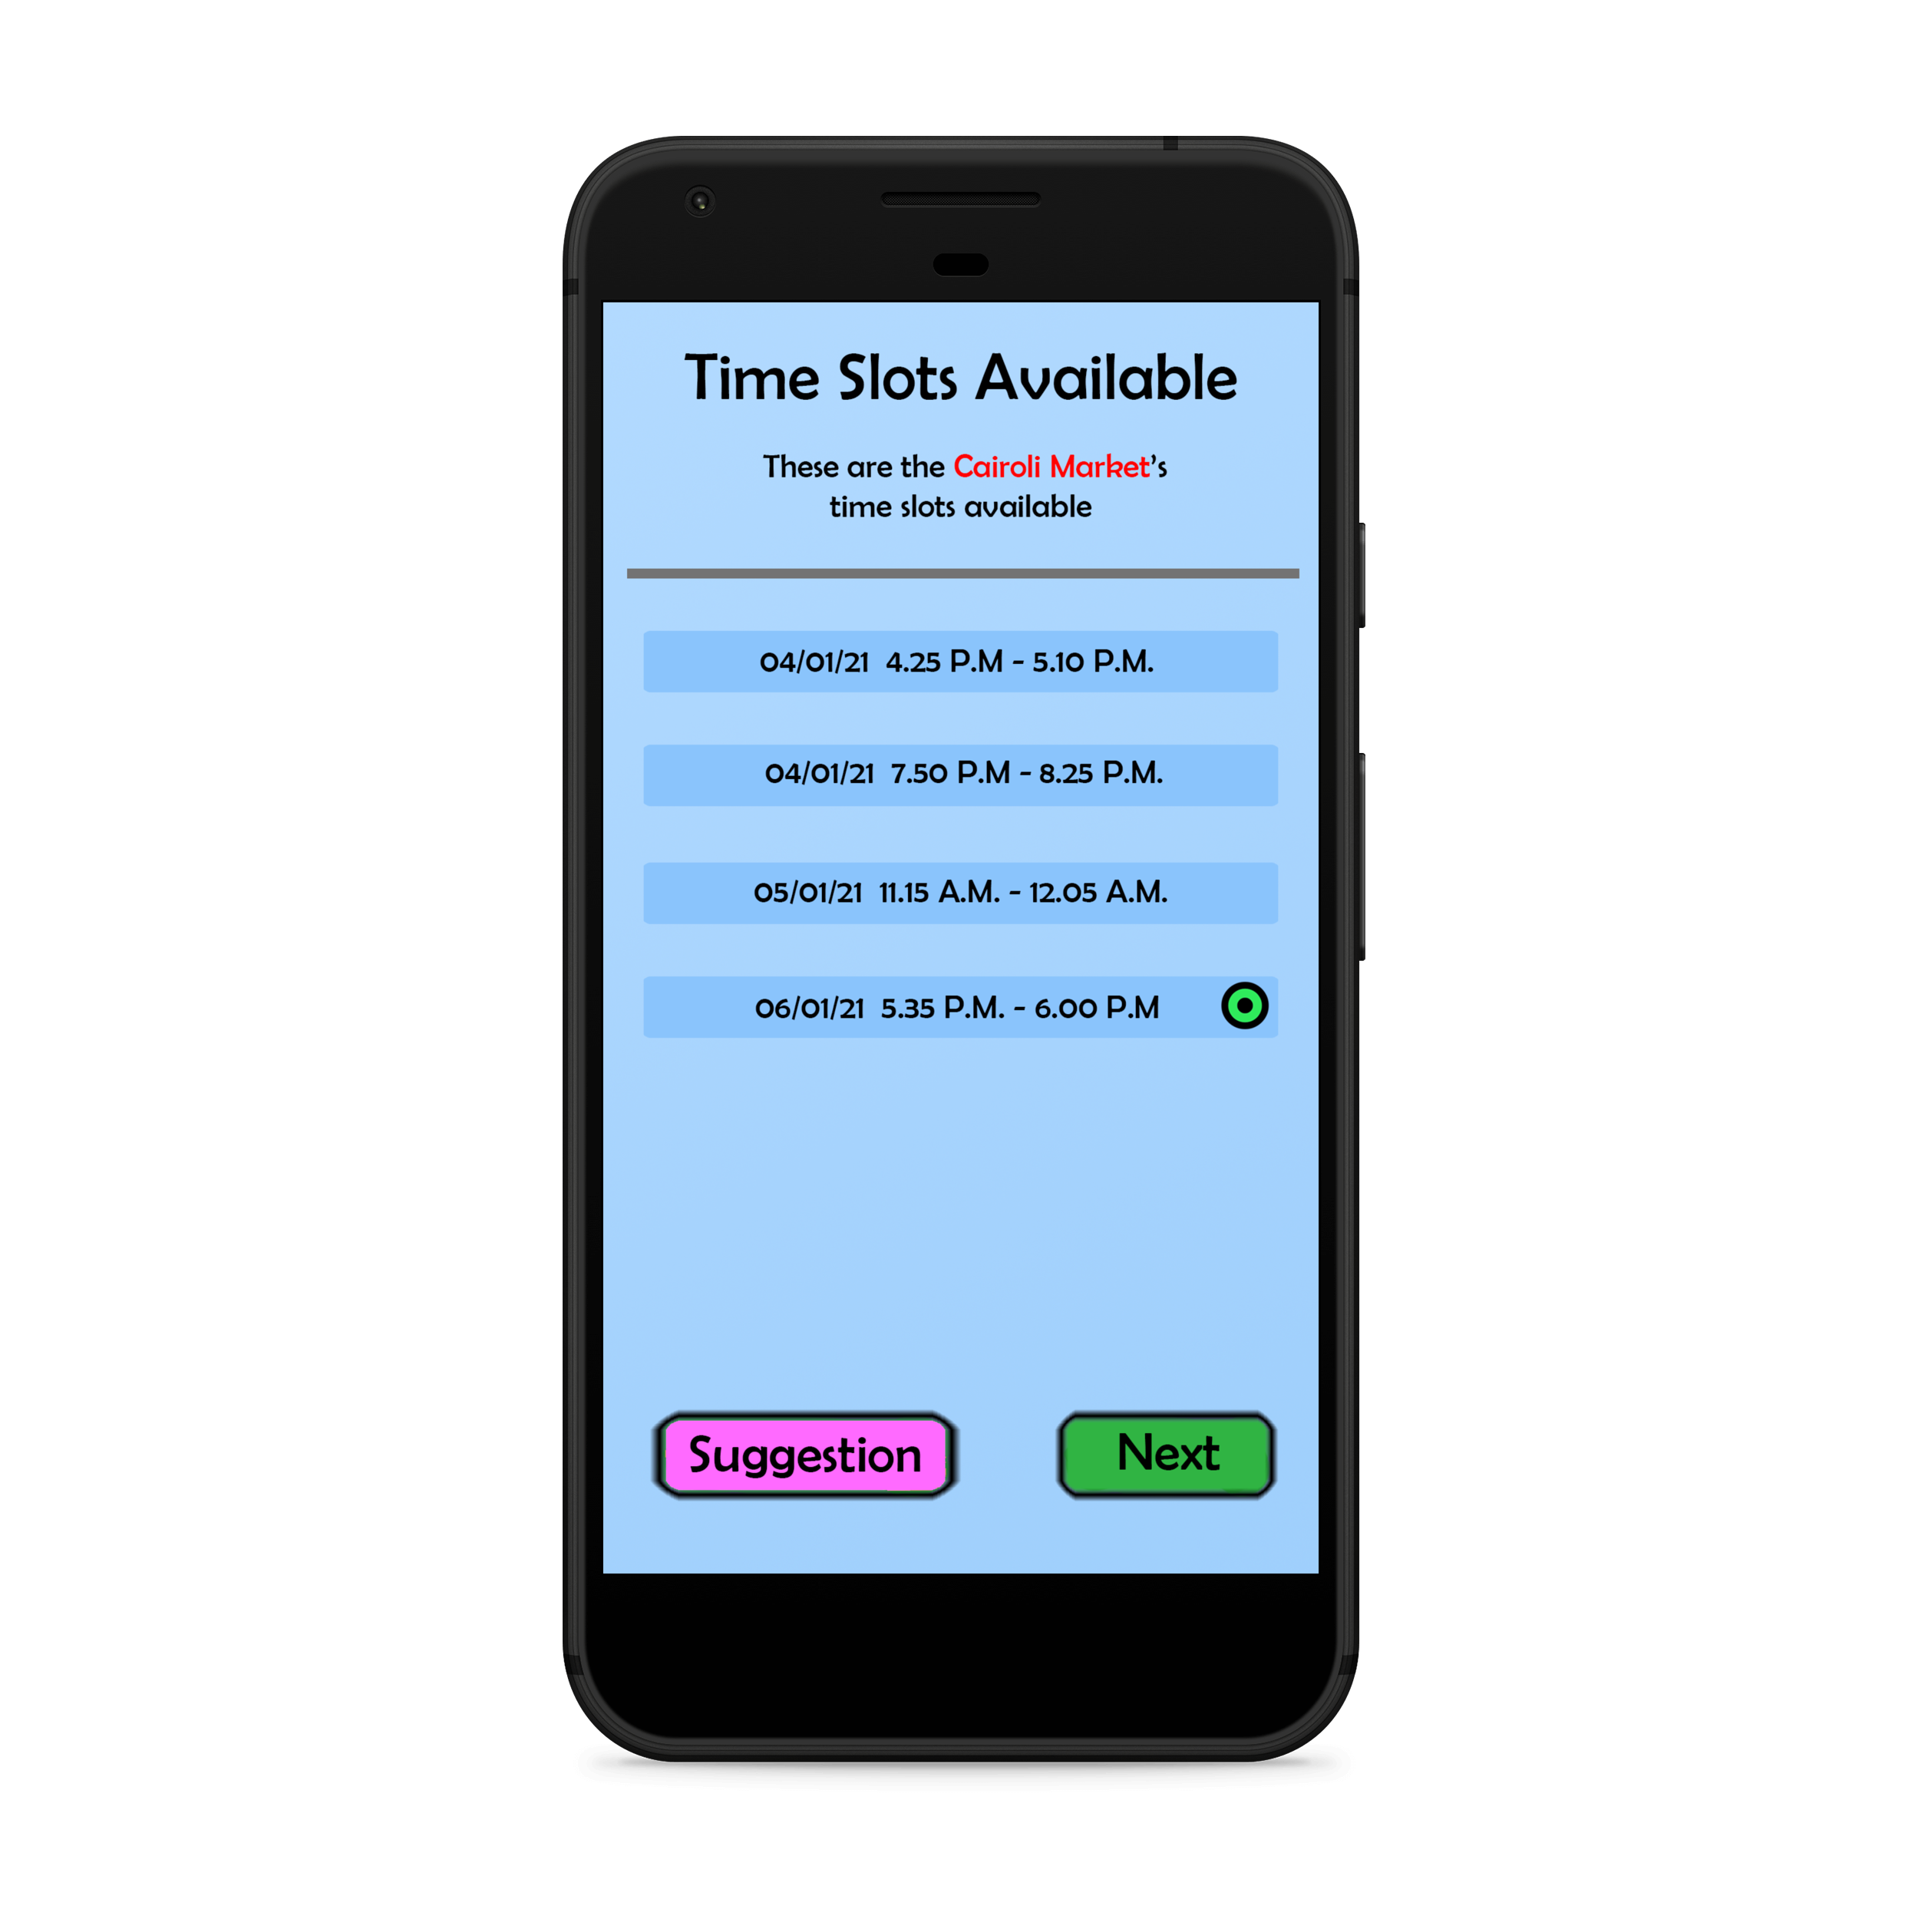
\includegraphics[scale=0.45]{../Mockups/TimeSlots.png}\\
			\end{adjustwidth}
			\caption{\emph{Choice of a time slot}}
		\end{figure}
	
		\begin{figure}[H]
		\begin{adjustwidth} {-4cm}{}
			\centering
			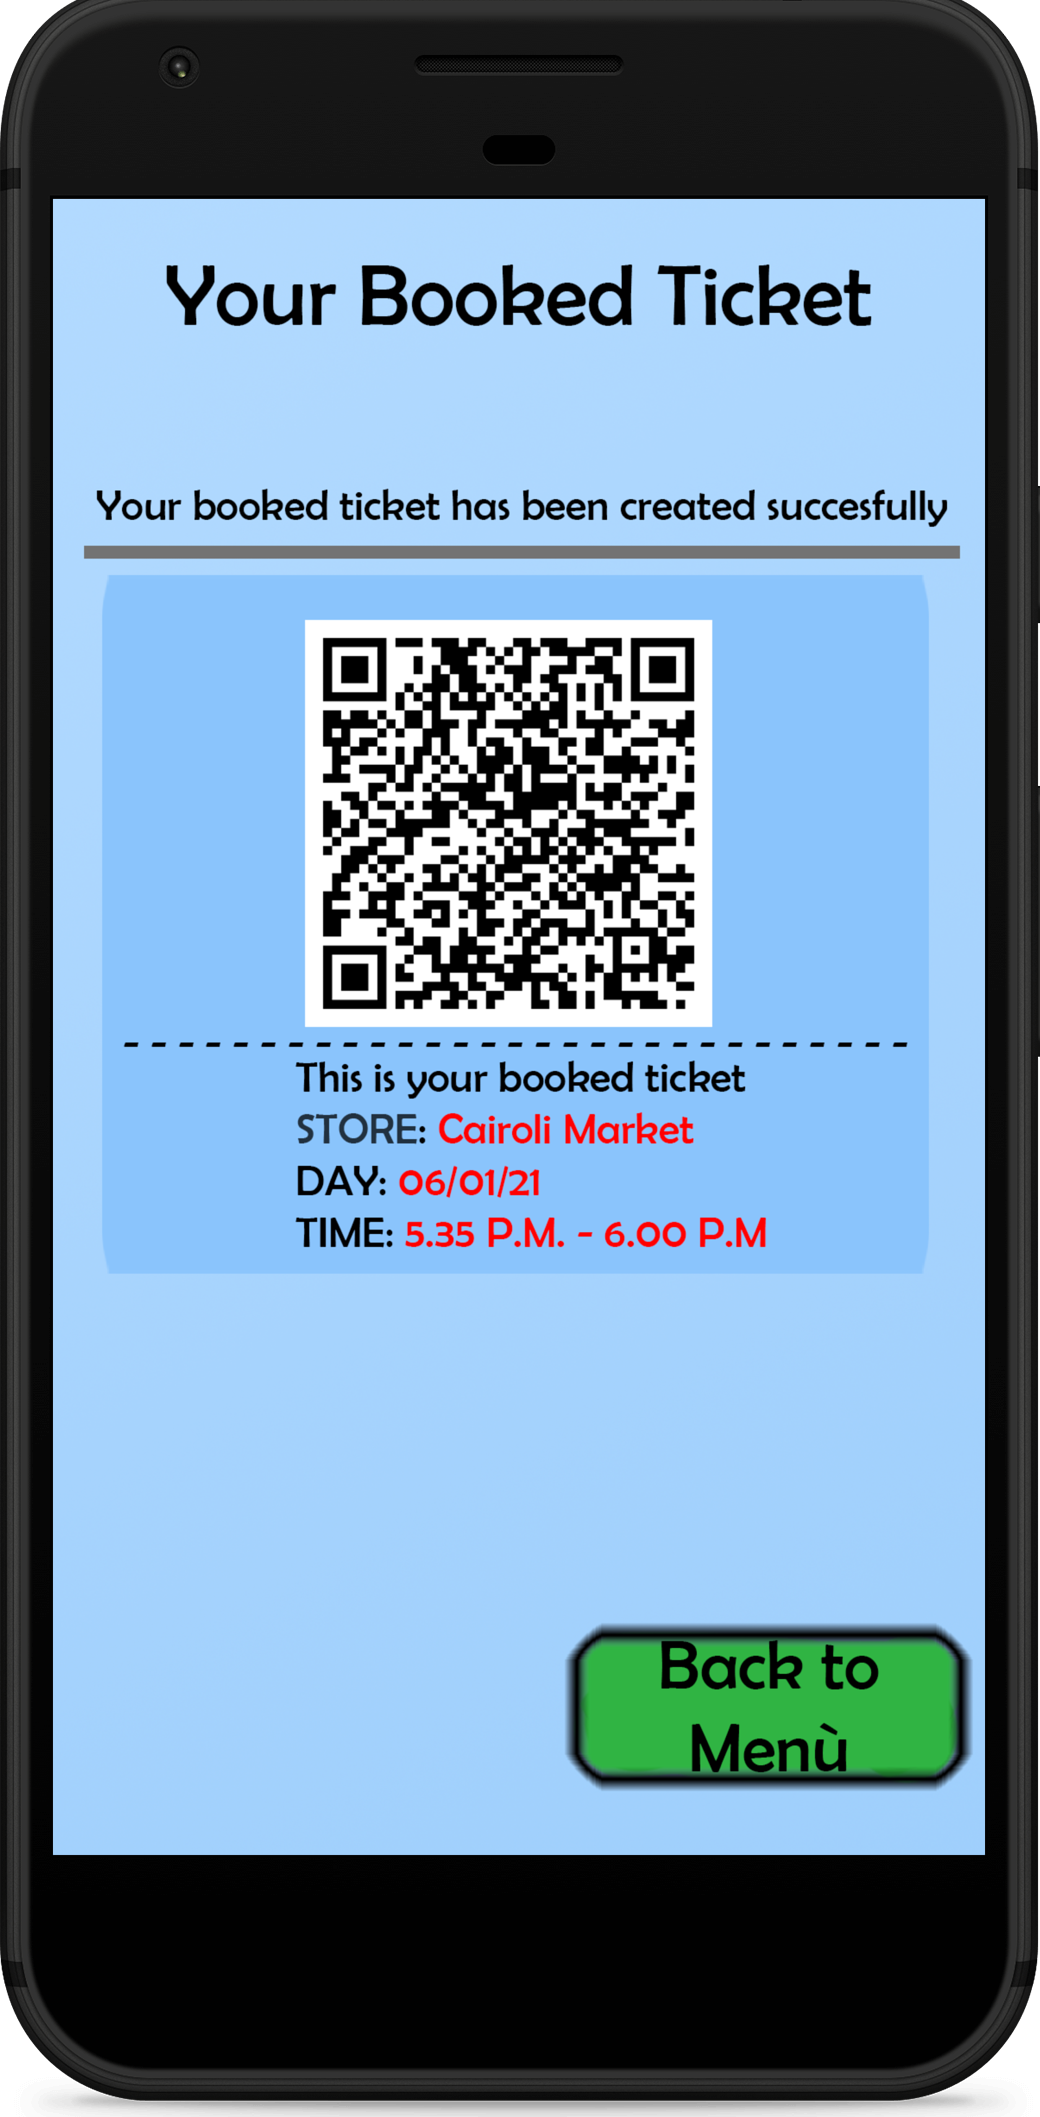
\includegraphics[scale=0.45]{../Mockups/BookedTicket.png}\\
		\end{adjustwidth}
		\caption{\emph{Creation of booked ticket}}
		\end{figure}
	
		\begin{figure}[H]
			\begin{adjustwidth} {-4cm}{}
				\centering
				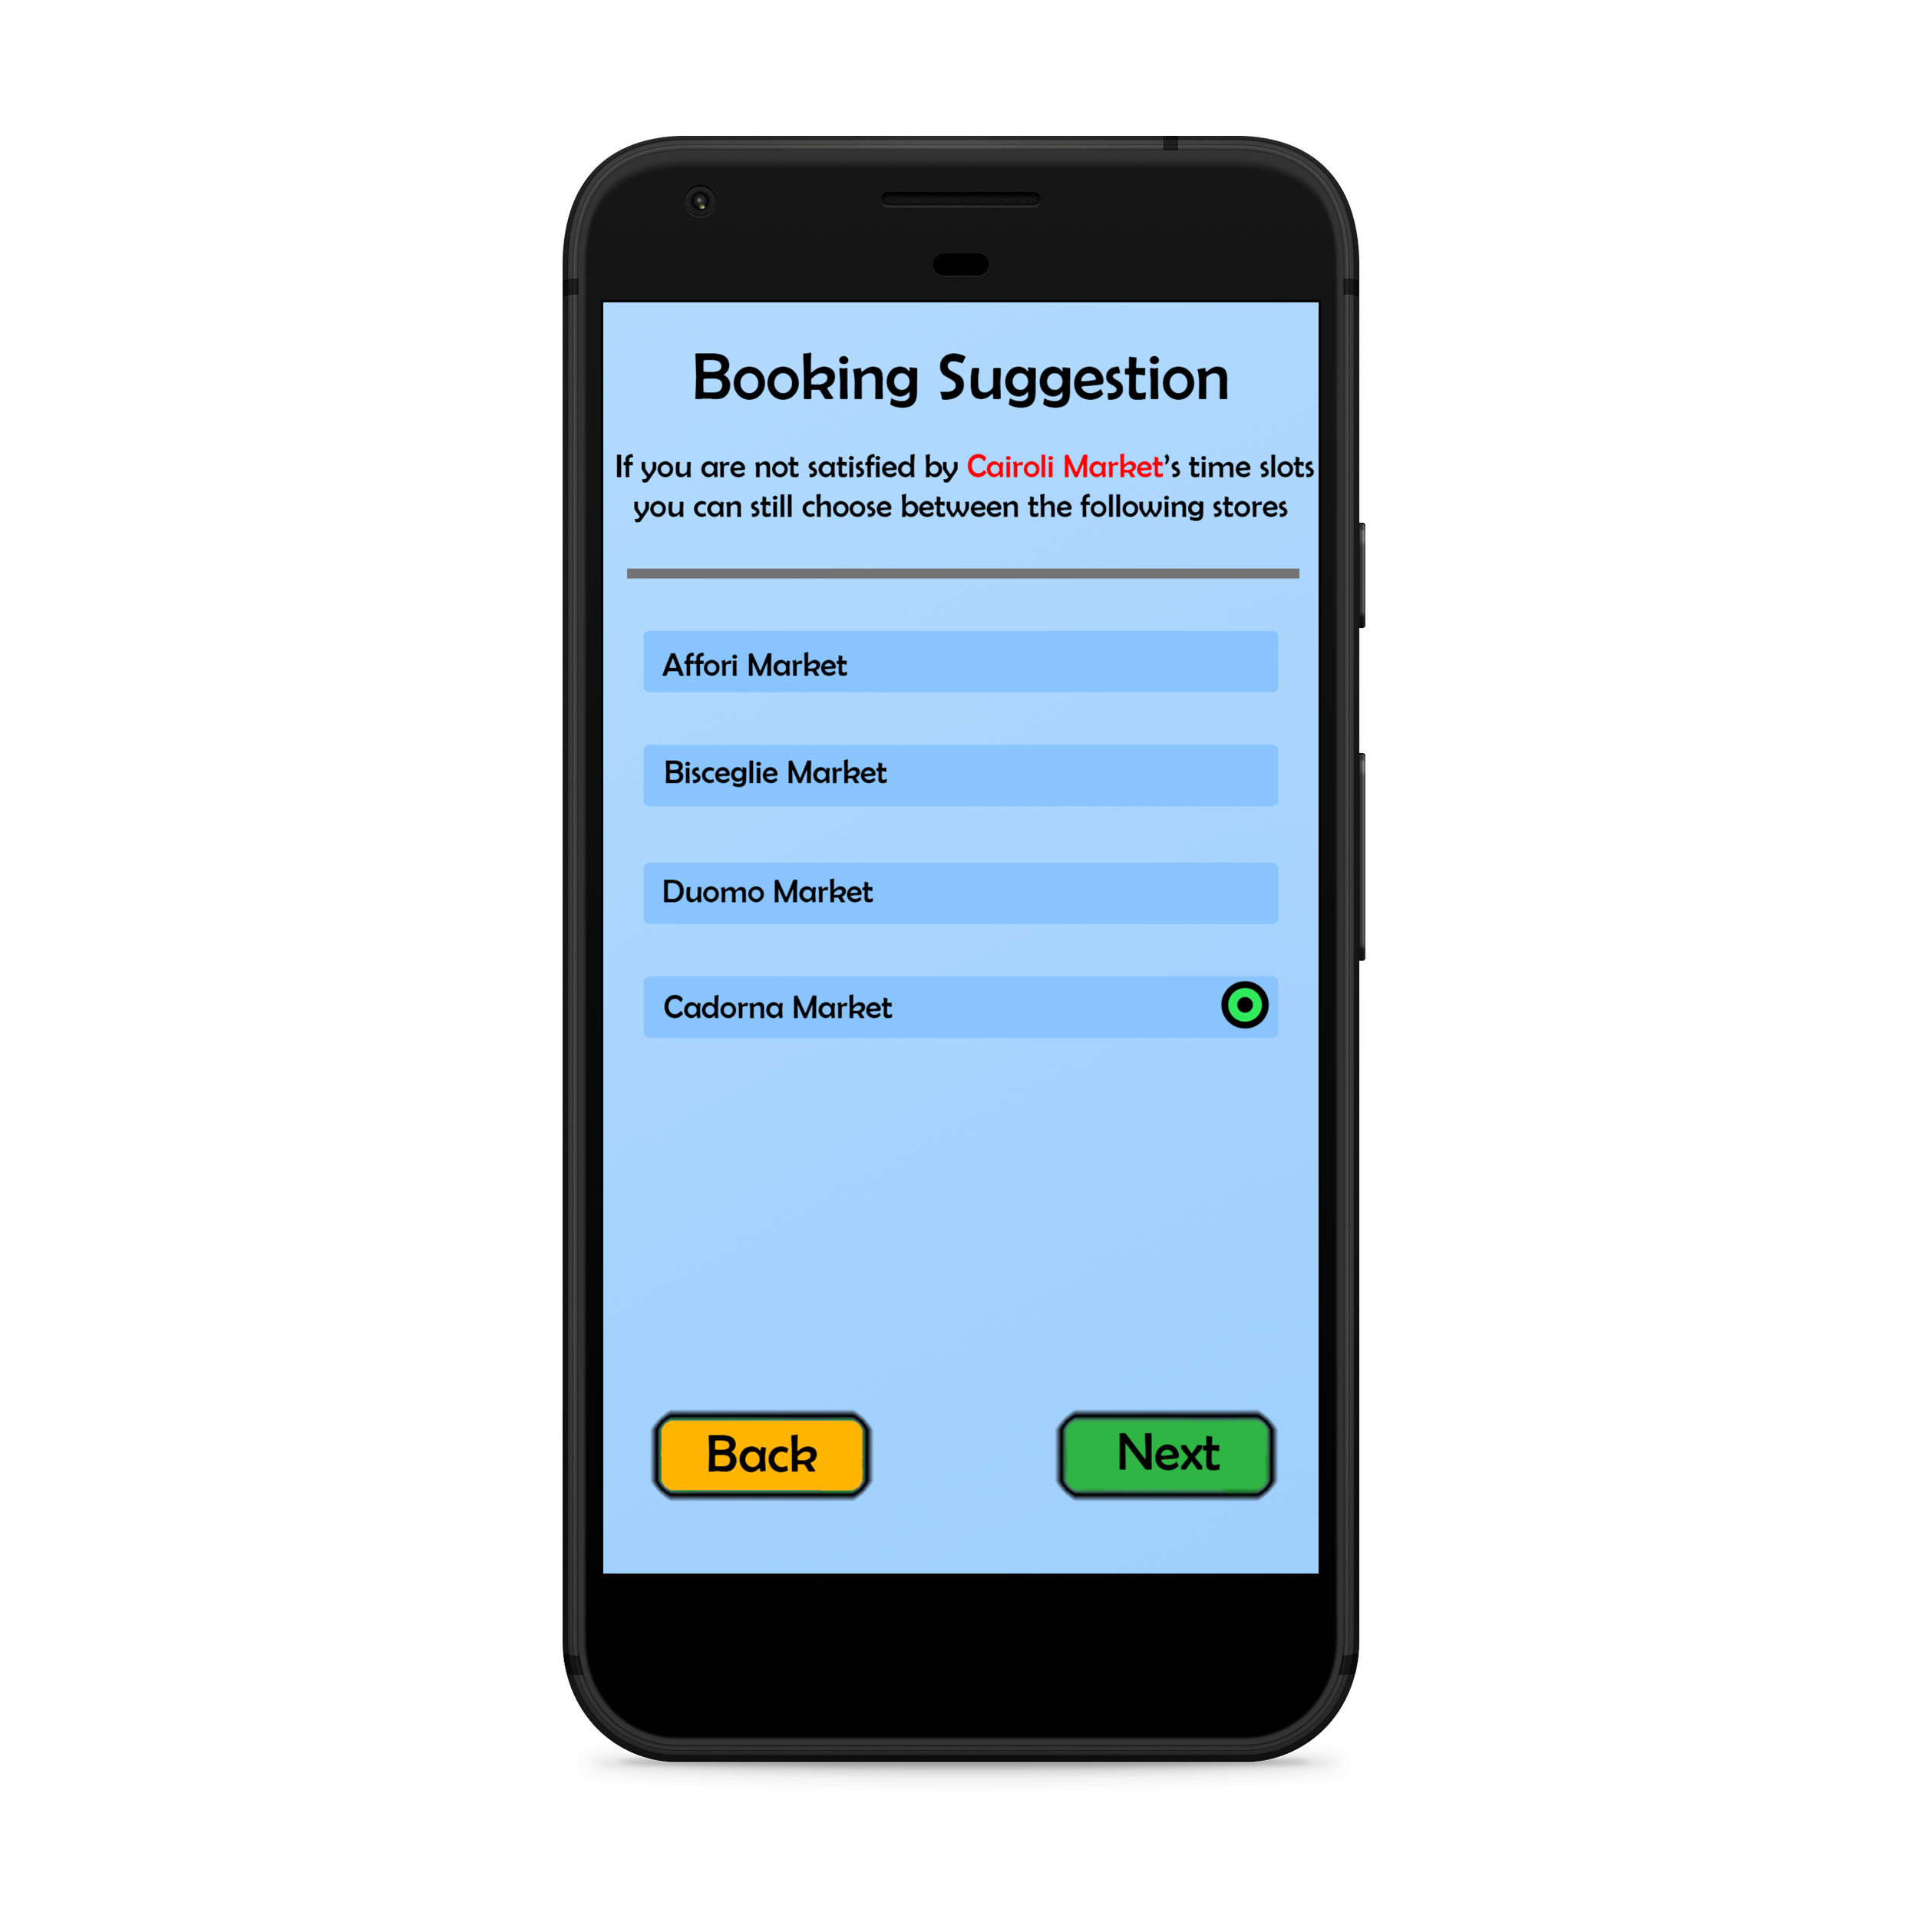
\includegraphics[scale=0.45]{../Mockups/BookingSuggestion.png}\\
			\end{adjustwidth}
			\caption{\emph{Booking suggestions}}
		\end{figure}
		
		\subsubsection{Show requests}
		
		Clicking on "Show requests" will bring us to Figure ???, where we can see all the reservation done through the application, and selecting one of them will show its complete ticket (Figure ???)
		
		\begin{figure}[H]
			\begin{adjustwidth} {-4cm}{}
				\centering
				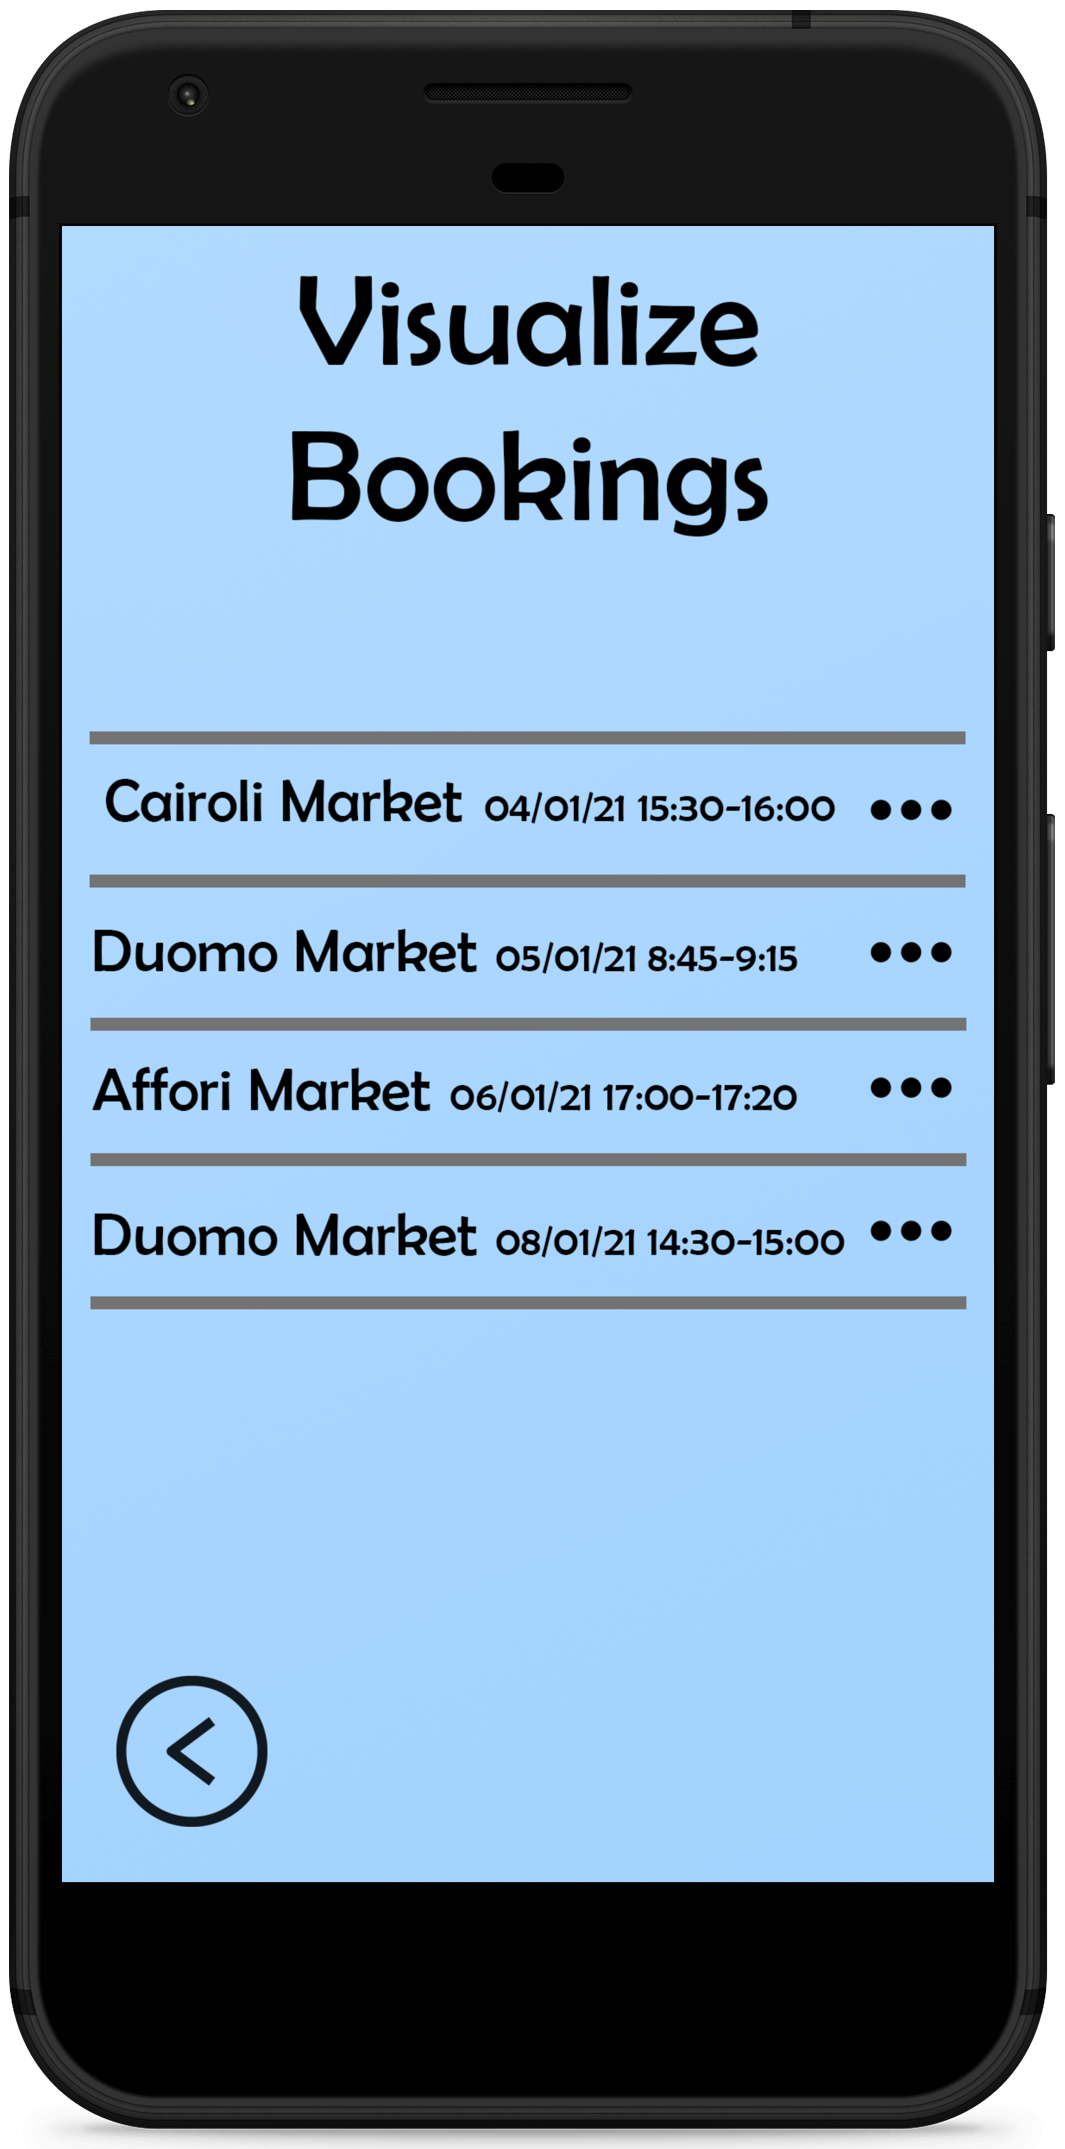
\includegraphics[scale=0.45]{../Mockups/VisualizeBookings.png}\\
			\end{adjustwidth}
			\caption{\emph{Show requests}}
		\end{figure}
	
		\begin{figure}[H]
			\begin{adjustwidth} {-4cm}{}
				\centering
				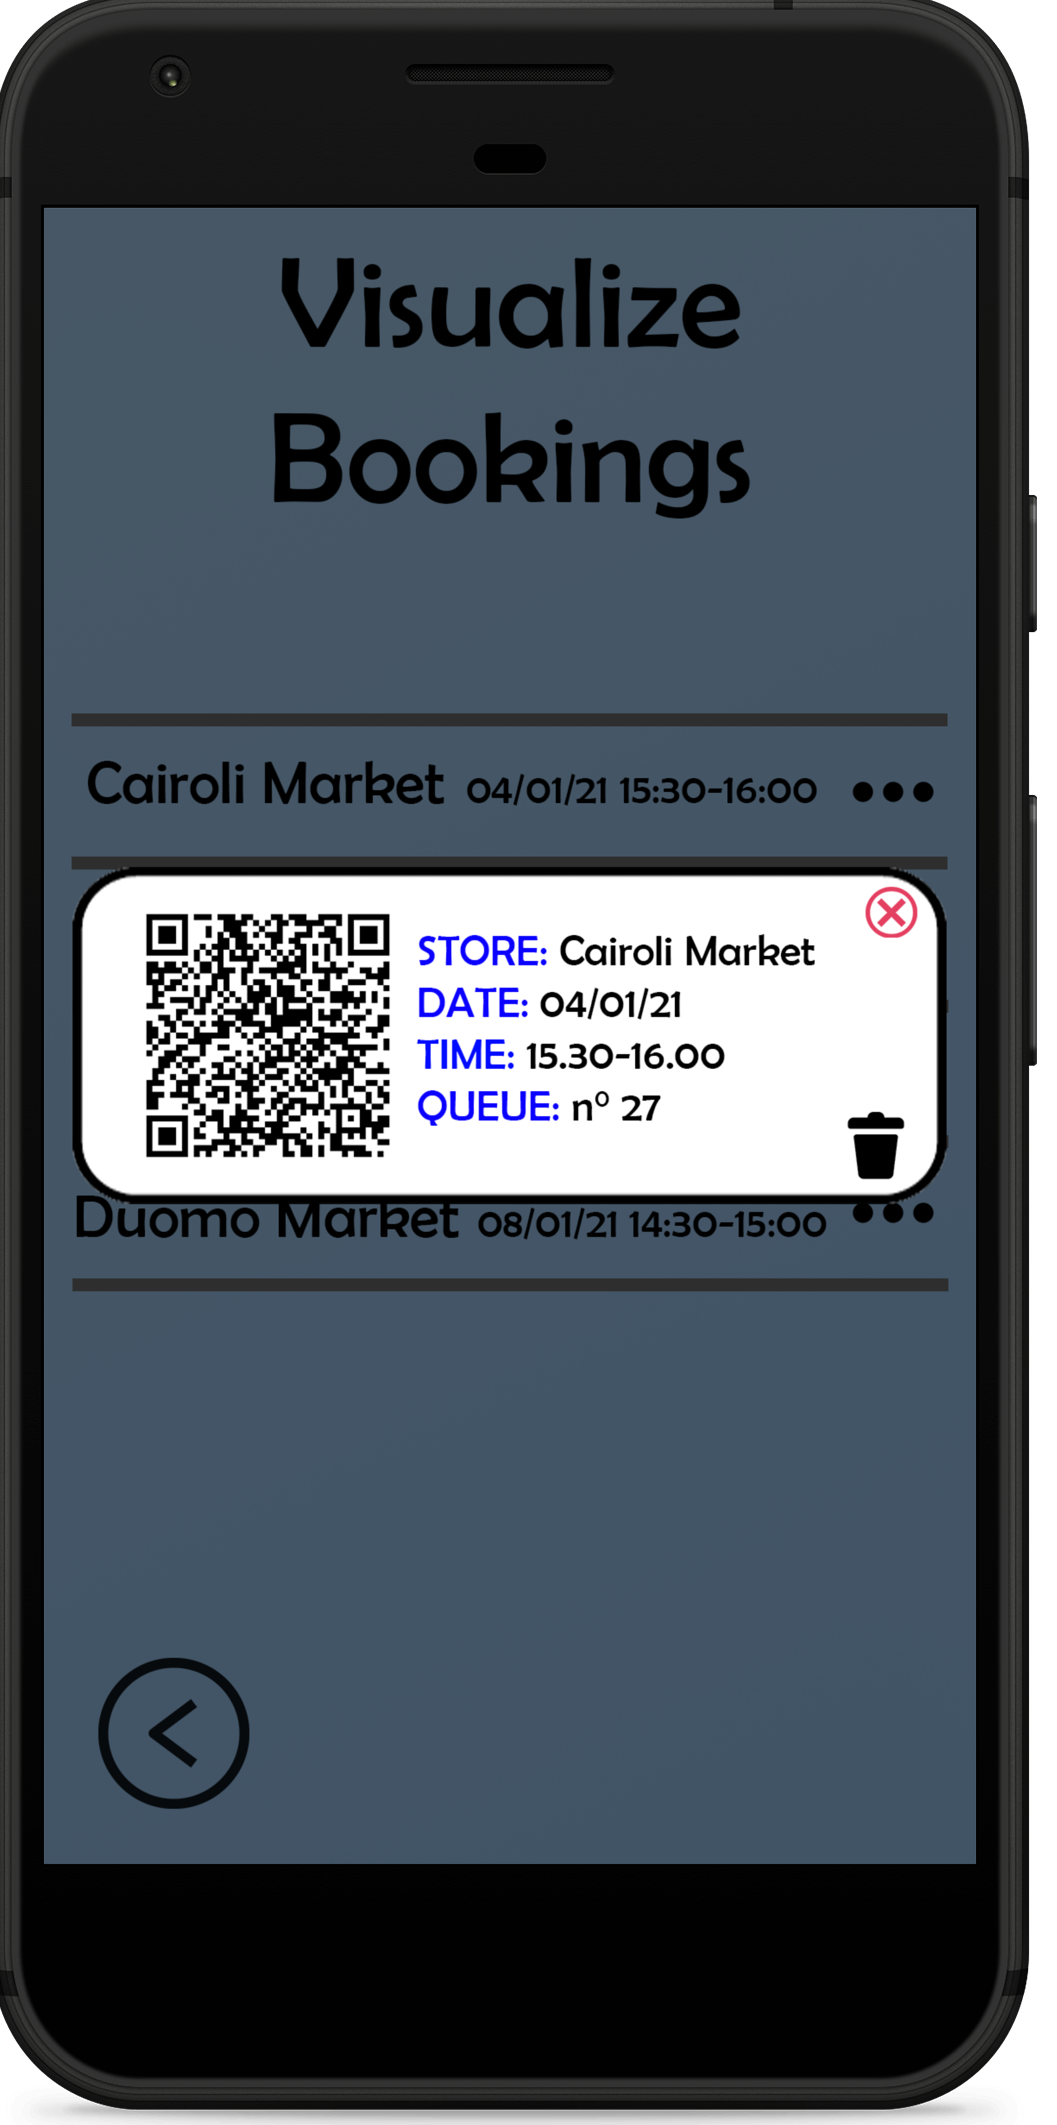
\includegraphics[scale=0.45]{../Mockups/VBpopup.png}\\
			\end{adjustwidth}
			\caption{\emph{Reservation details}}
		\end{figure}
		
		\subsubsection{Means of Transport}
		
		Clicking on "Means of transport" will bring us to Figure ???, where we can choose our mean of transport (it will be used by the system to calculate the estimated time the customer will need to reach the store, thus the time he will be notified)
		
		\begin{figure}[H]
			\begin{adjustwidth} {-4cm}{}
				\centering
				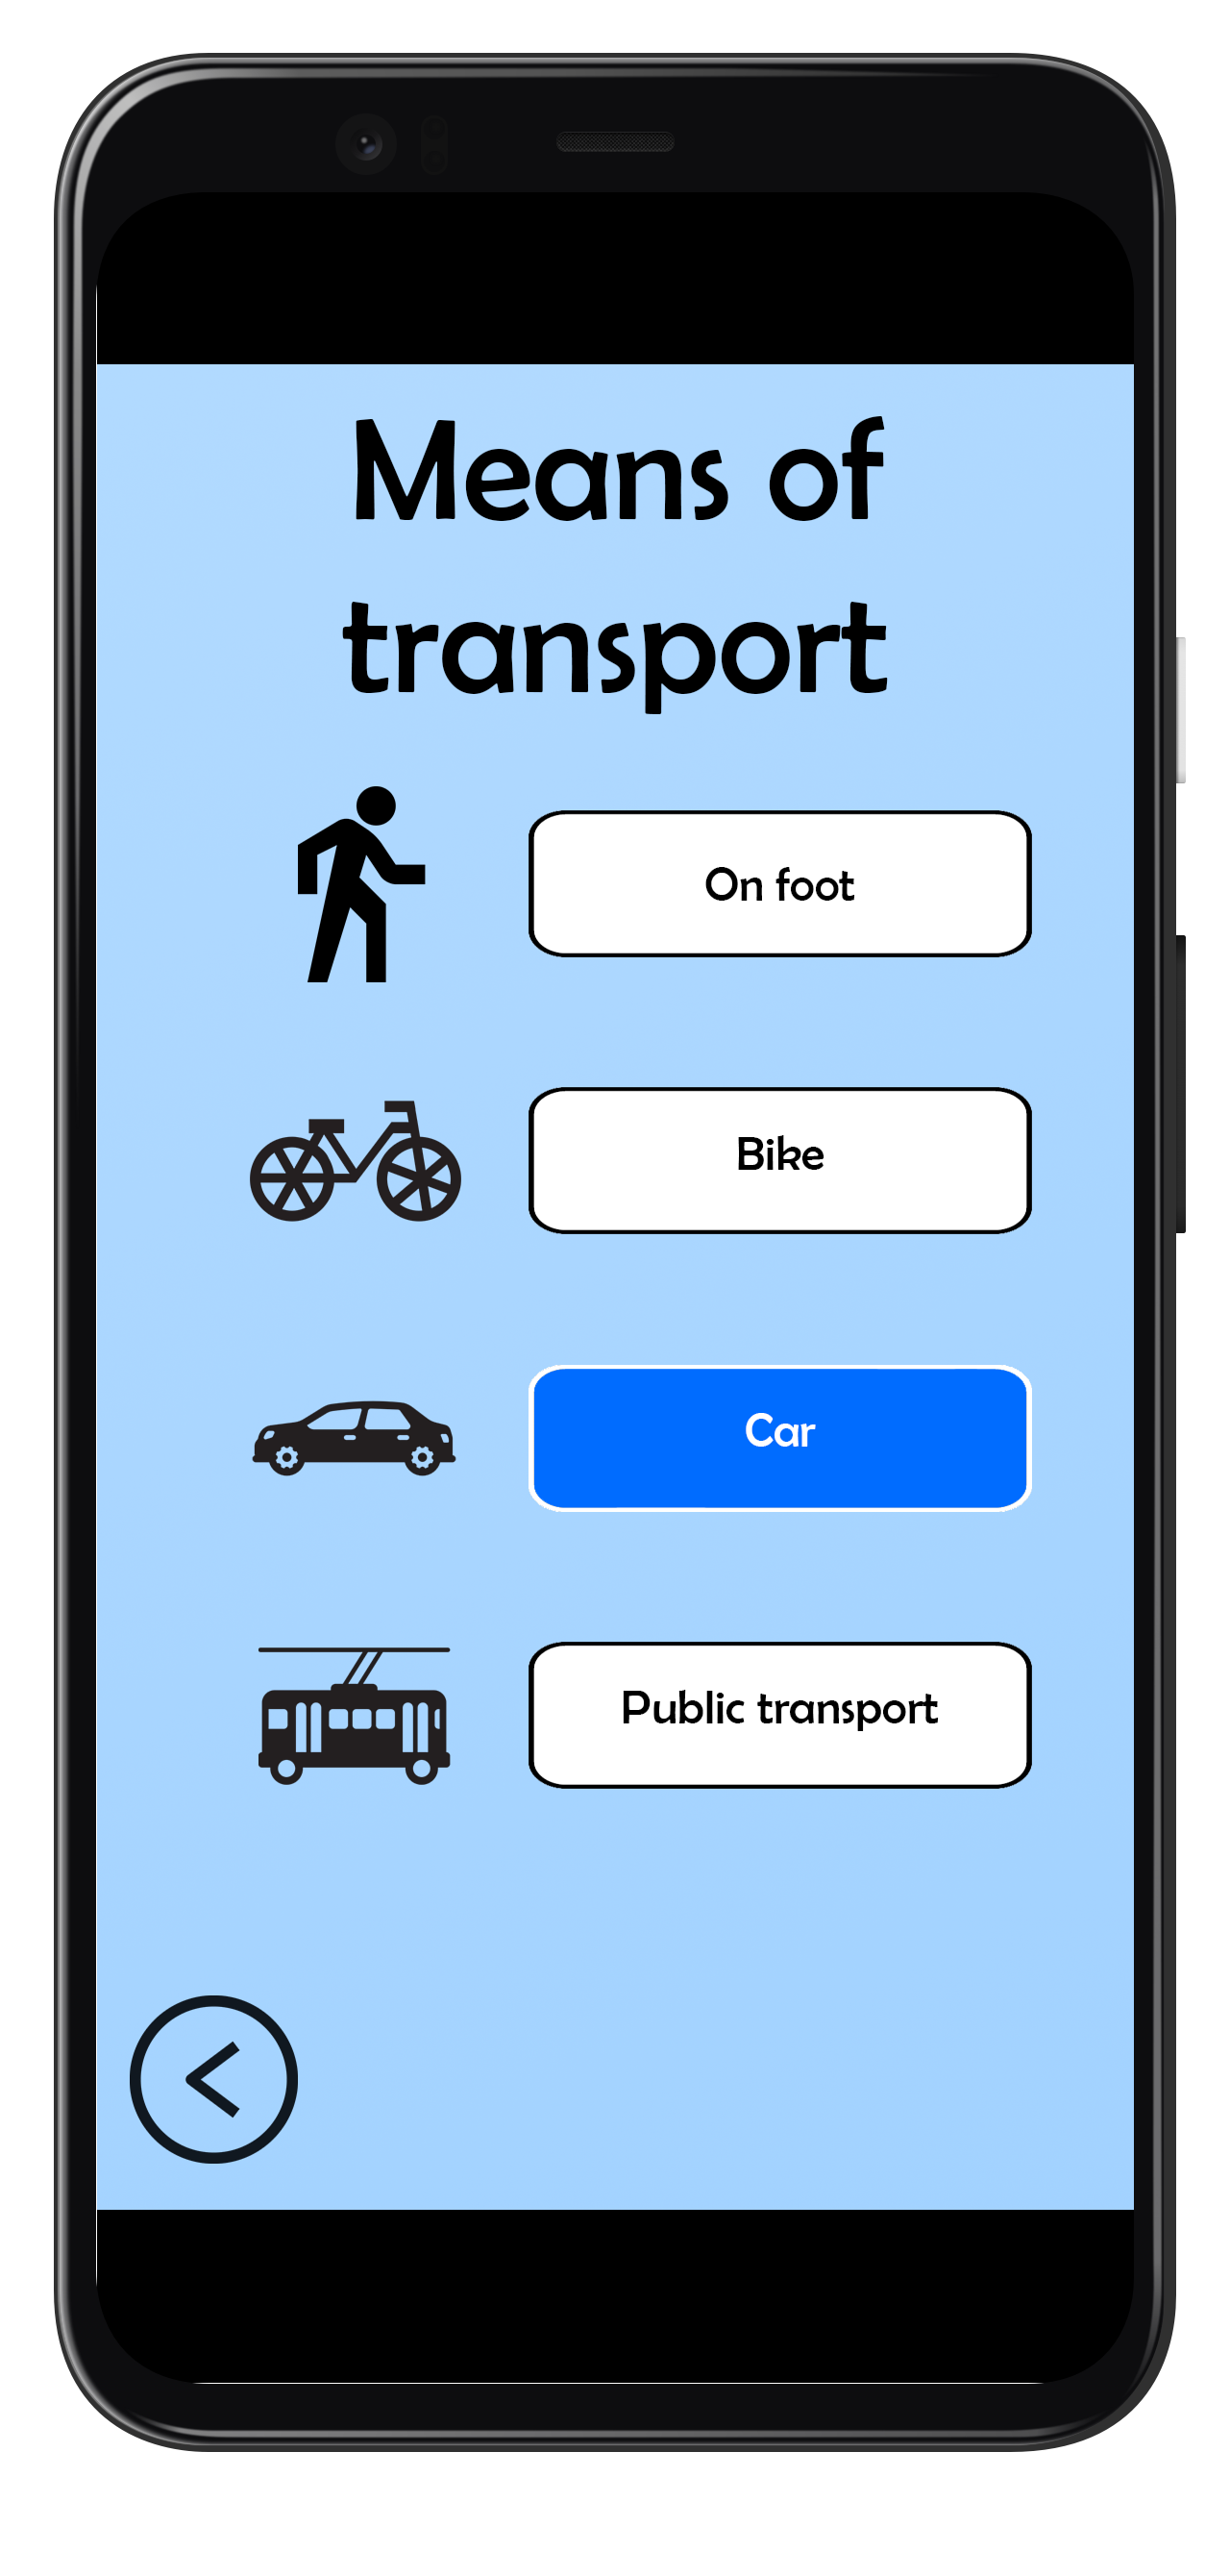
\includegraphics[scale=0.45]{../Mockups/MeansOfTransport.png}\\
			\end{adjustwidth}
			\caption{\emph{Means of transport}}
		\end{figure}

		
		
	\subsection{Store Manager POV}
		\subsubsection{Registration and Login}
		We start from the mockup in Figure ??? also in the store manager POV.
		
		Clicking on "Sign up as store" will bring us to Figure ???, in which a new (unregistered) store manager has to enter his store's data (Store name, a password, the store capacity and the store certification), and can already add departments to his new account with the "Add department" button; in the end, he can click "Sign up" in order to create the account.
		
		Clicking on "Login as store" will bring us to Figure ???, in which a store manager can enter his store's ID and password in order to log in.
		
		\begin{figure}[H]
			\begin{adjustwidth} {-4cm}{}
				\centering
				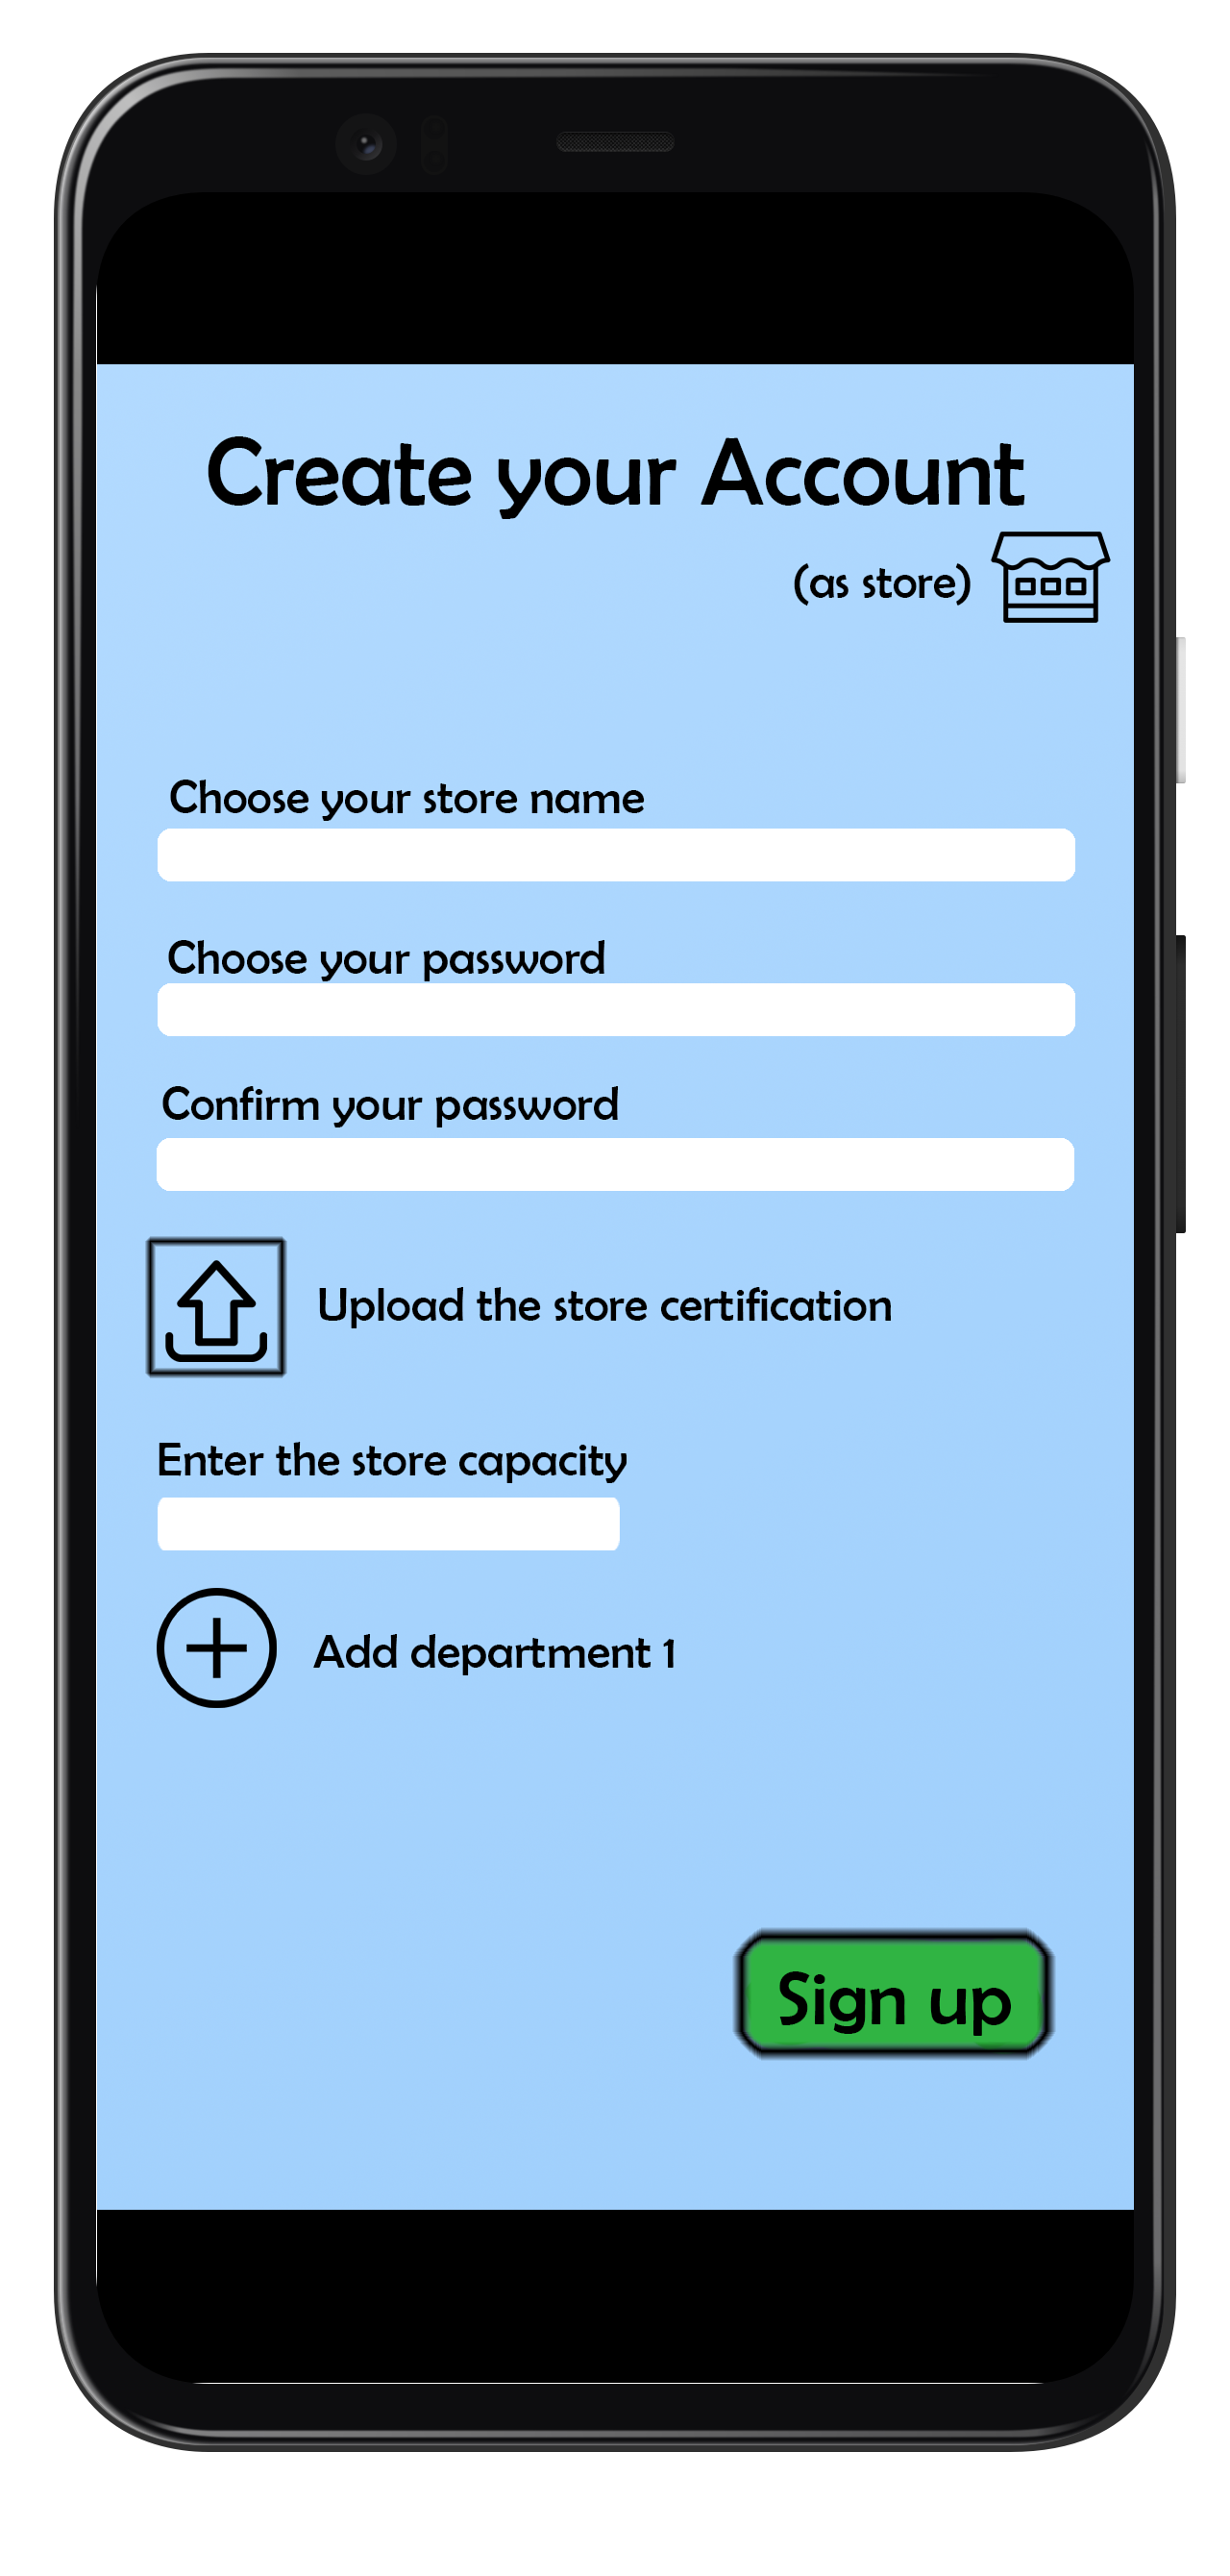
\includegraphics[scale=0.45]{../Mockups/SignUpStore.png}\\
			\end{adjustwidth}
			\caption{\emph{Sign up as a store}}
		\end{figure}
	
		\begin{figure}[H]
			\begin{adjustwidth} {-4cm}{}
				\centering
				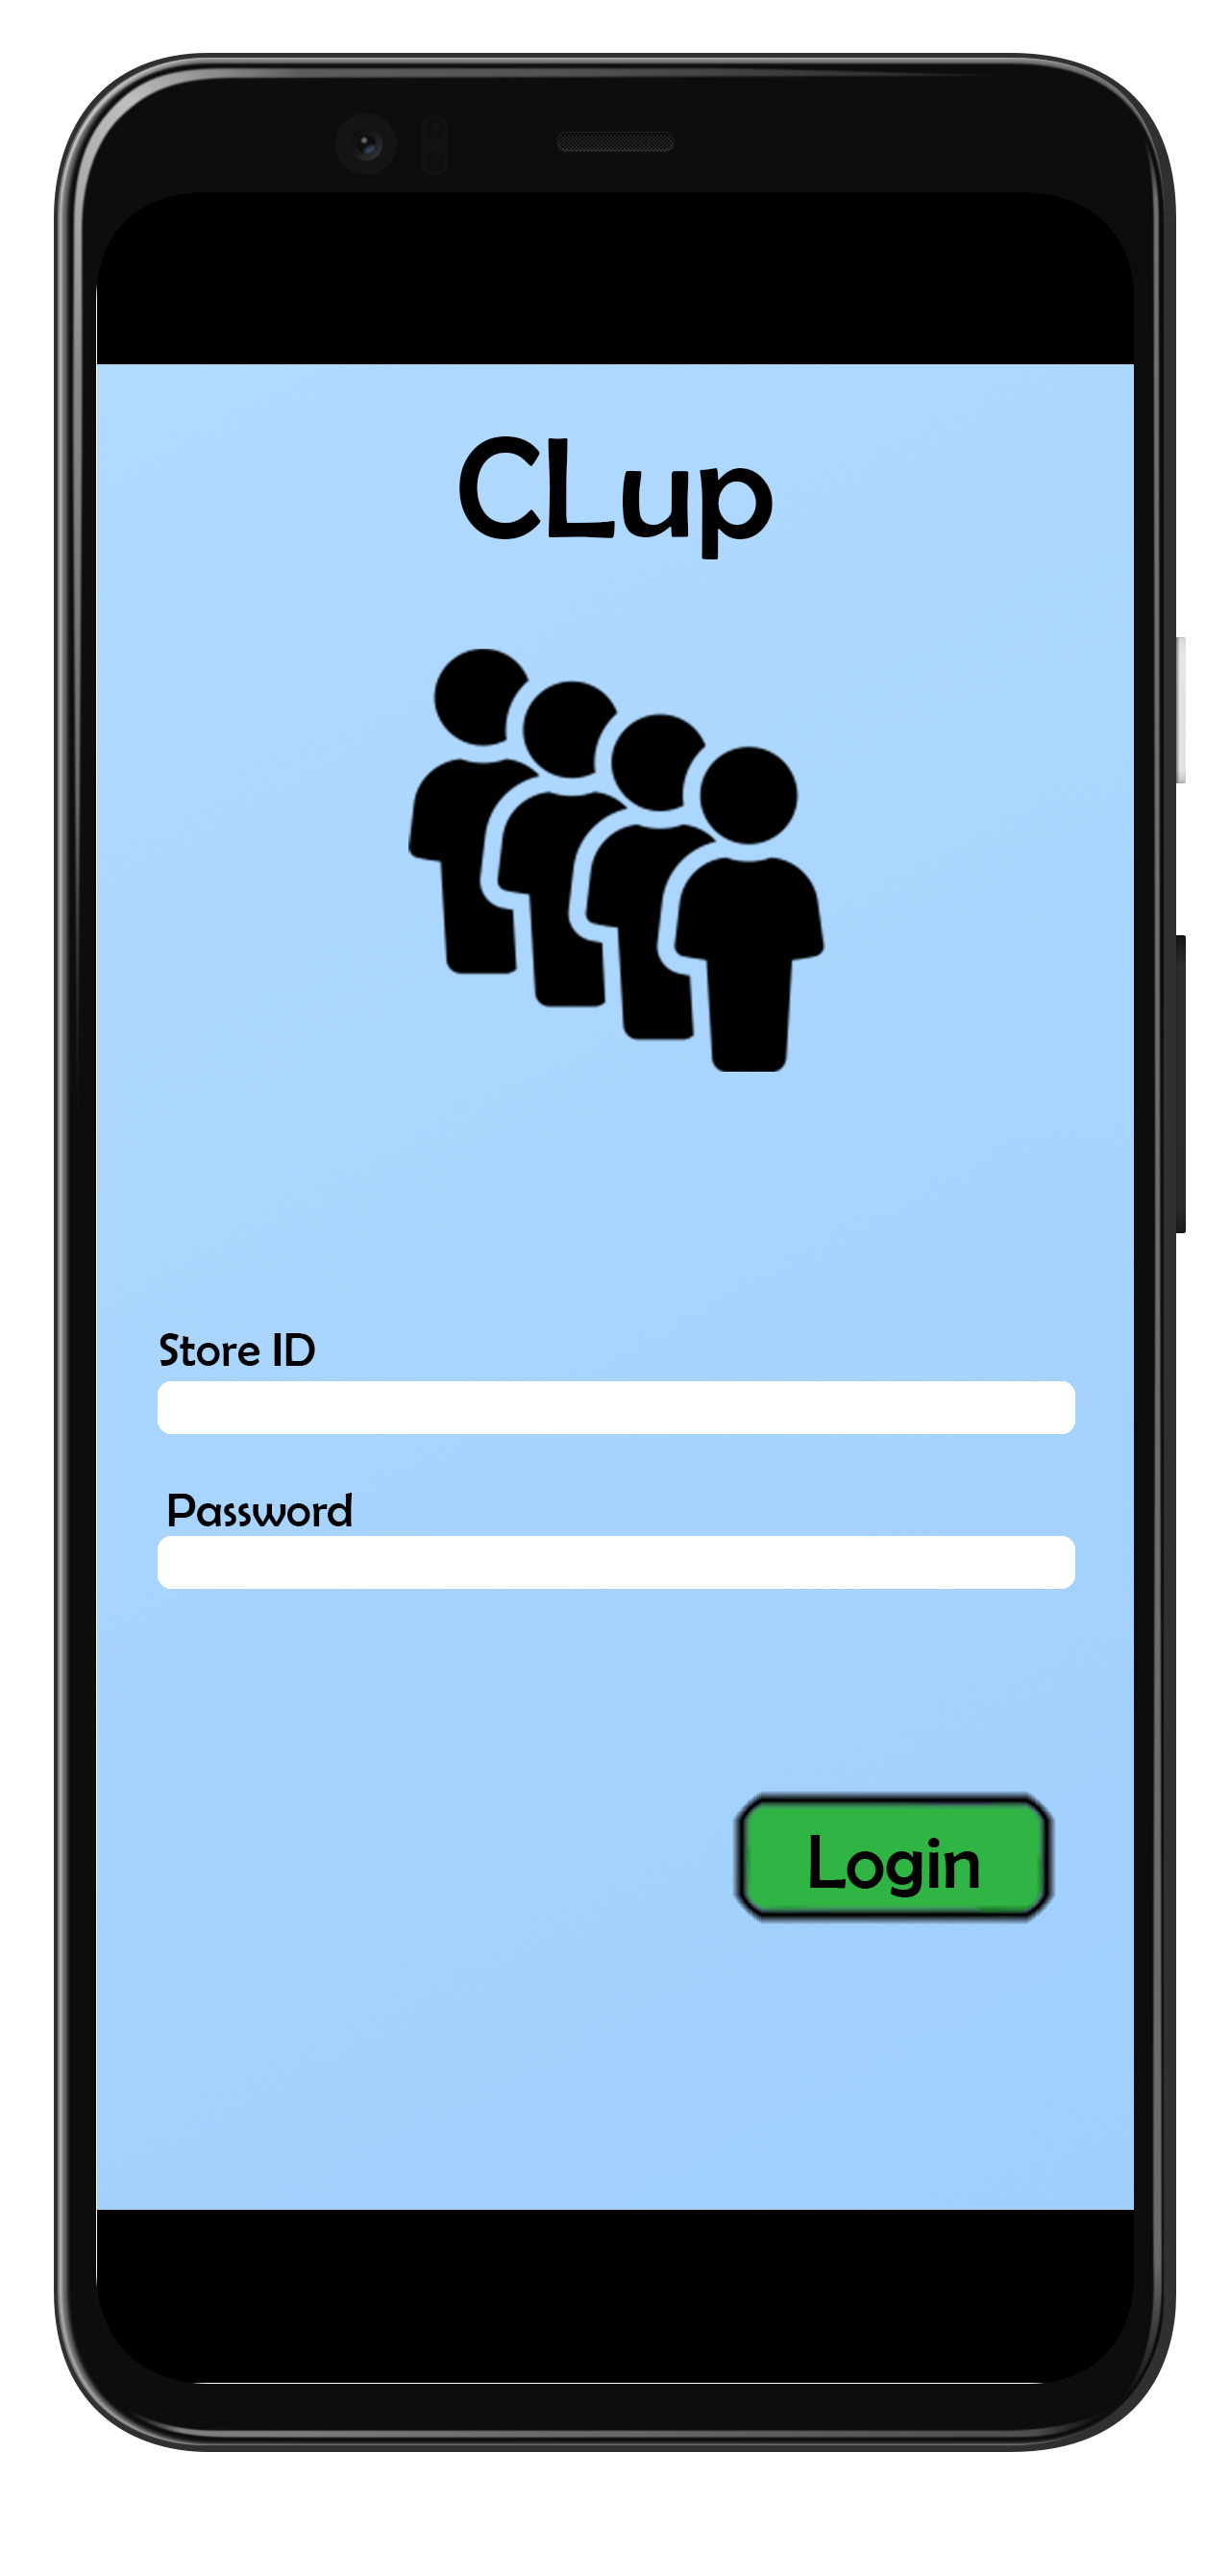
\includegraphics[scale=0.45]{../Mockups/LoginStore.png}\\
			\end{adjustwidth}
			\caption{\emph{Login as a store}}
		\end{figure}
		
		\subsubsection{Manage bookings}
		
		Clicking on "Manage bookings" will bring us to Figure ???, in which we can see all the future reservations of our store, and selecting one of them will show us some possible actions (Figure ???):
		
			- "Contact Client" allow us to send an email to the customer that made the selected reservation;
			
			- "Cancel Booking" allow us to delete the selected reservation and send an email to the customer that made that reservation (justifying the deletion);
			
			- "Reschedule Booking" allow us to change date and time of the selected reservation
			
			\begin{figure}[H]
			\begin{adjustwidth} {-4cm}{}
				\centering
				\includegraphics[scale=0.45]{../Mockups/ManageBooking.png}\\
			\end{adjustwidth}
			\caption{\emph{Manage reservations}}
			\end{figure}
		
			\begin{figure}[H]
				\begin{adjustwidth} {-4cm}{}
					\centering
					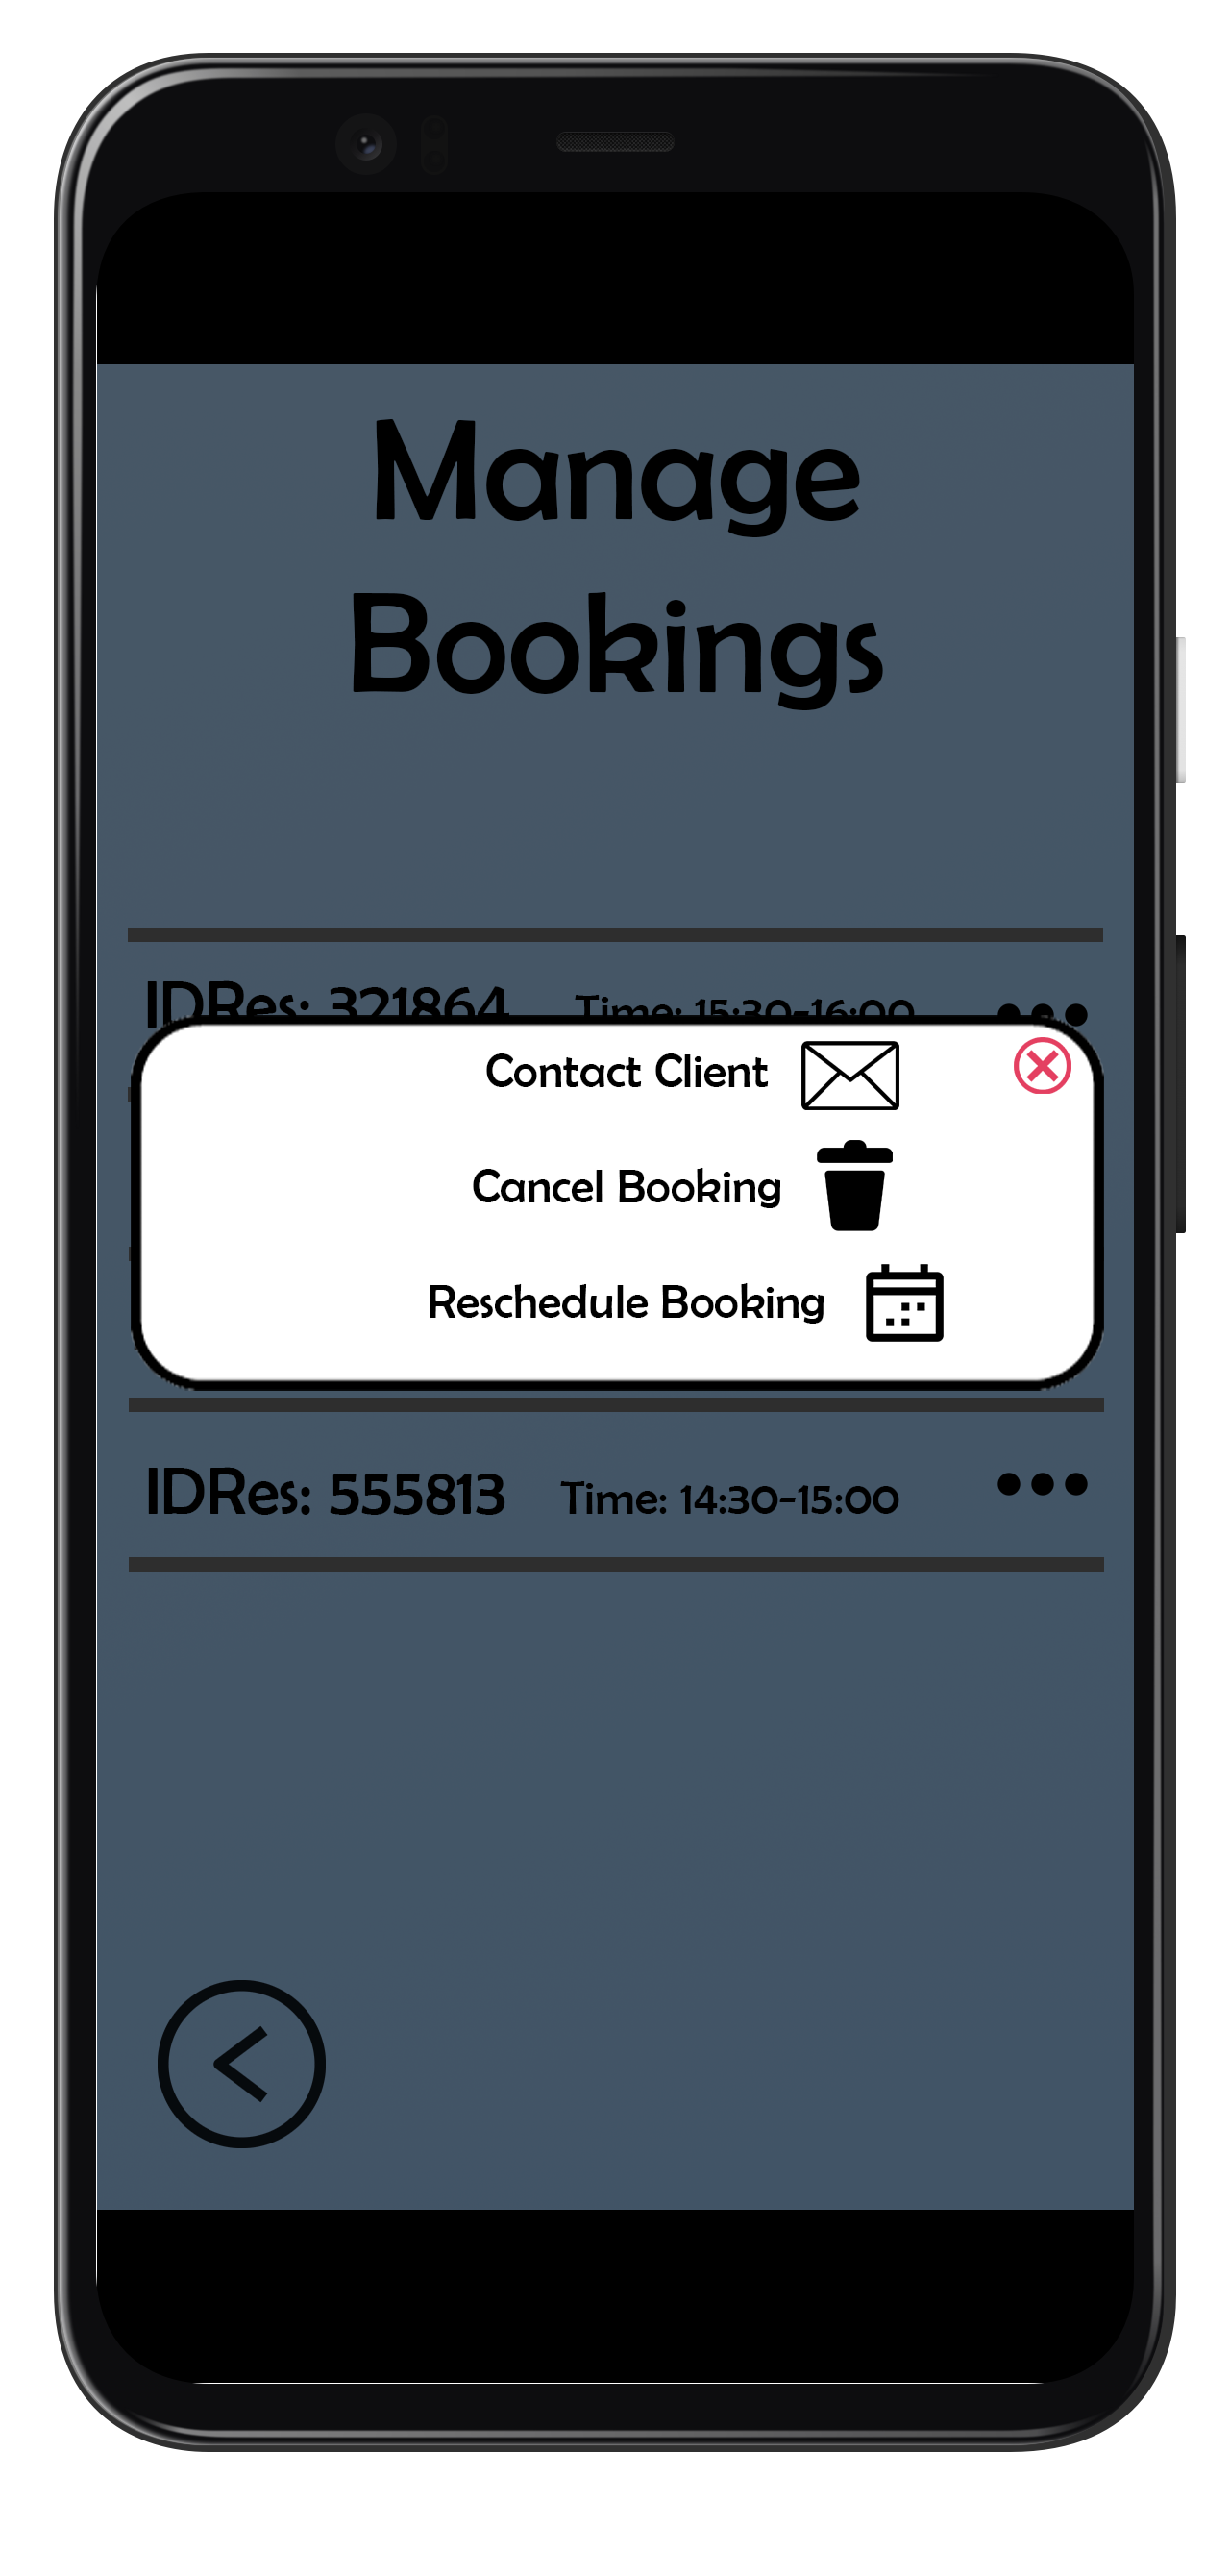
\includegraphics[scale=0.45]{../Mockups/MBpopup.png}\\
				\end{adjustwidth}
				\caption{\emph{Possible actions for the selected reservation}}
			\end{figure}
		
			\begin{figure}[H]
				\begin{adjustwidth} {-4cm}{}
					\centering
					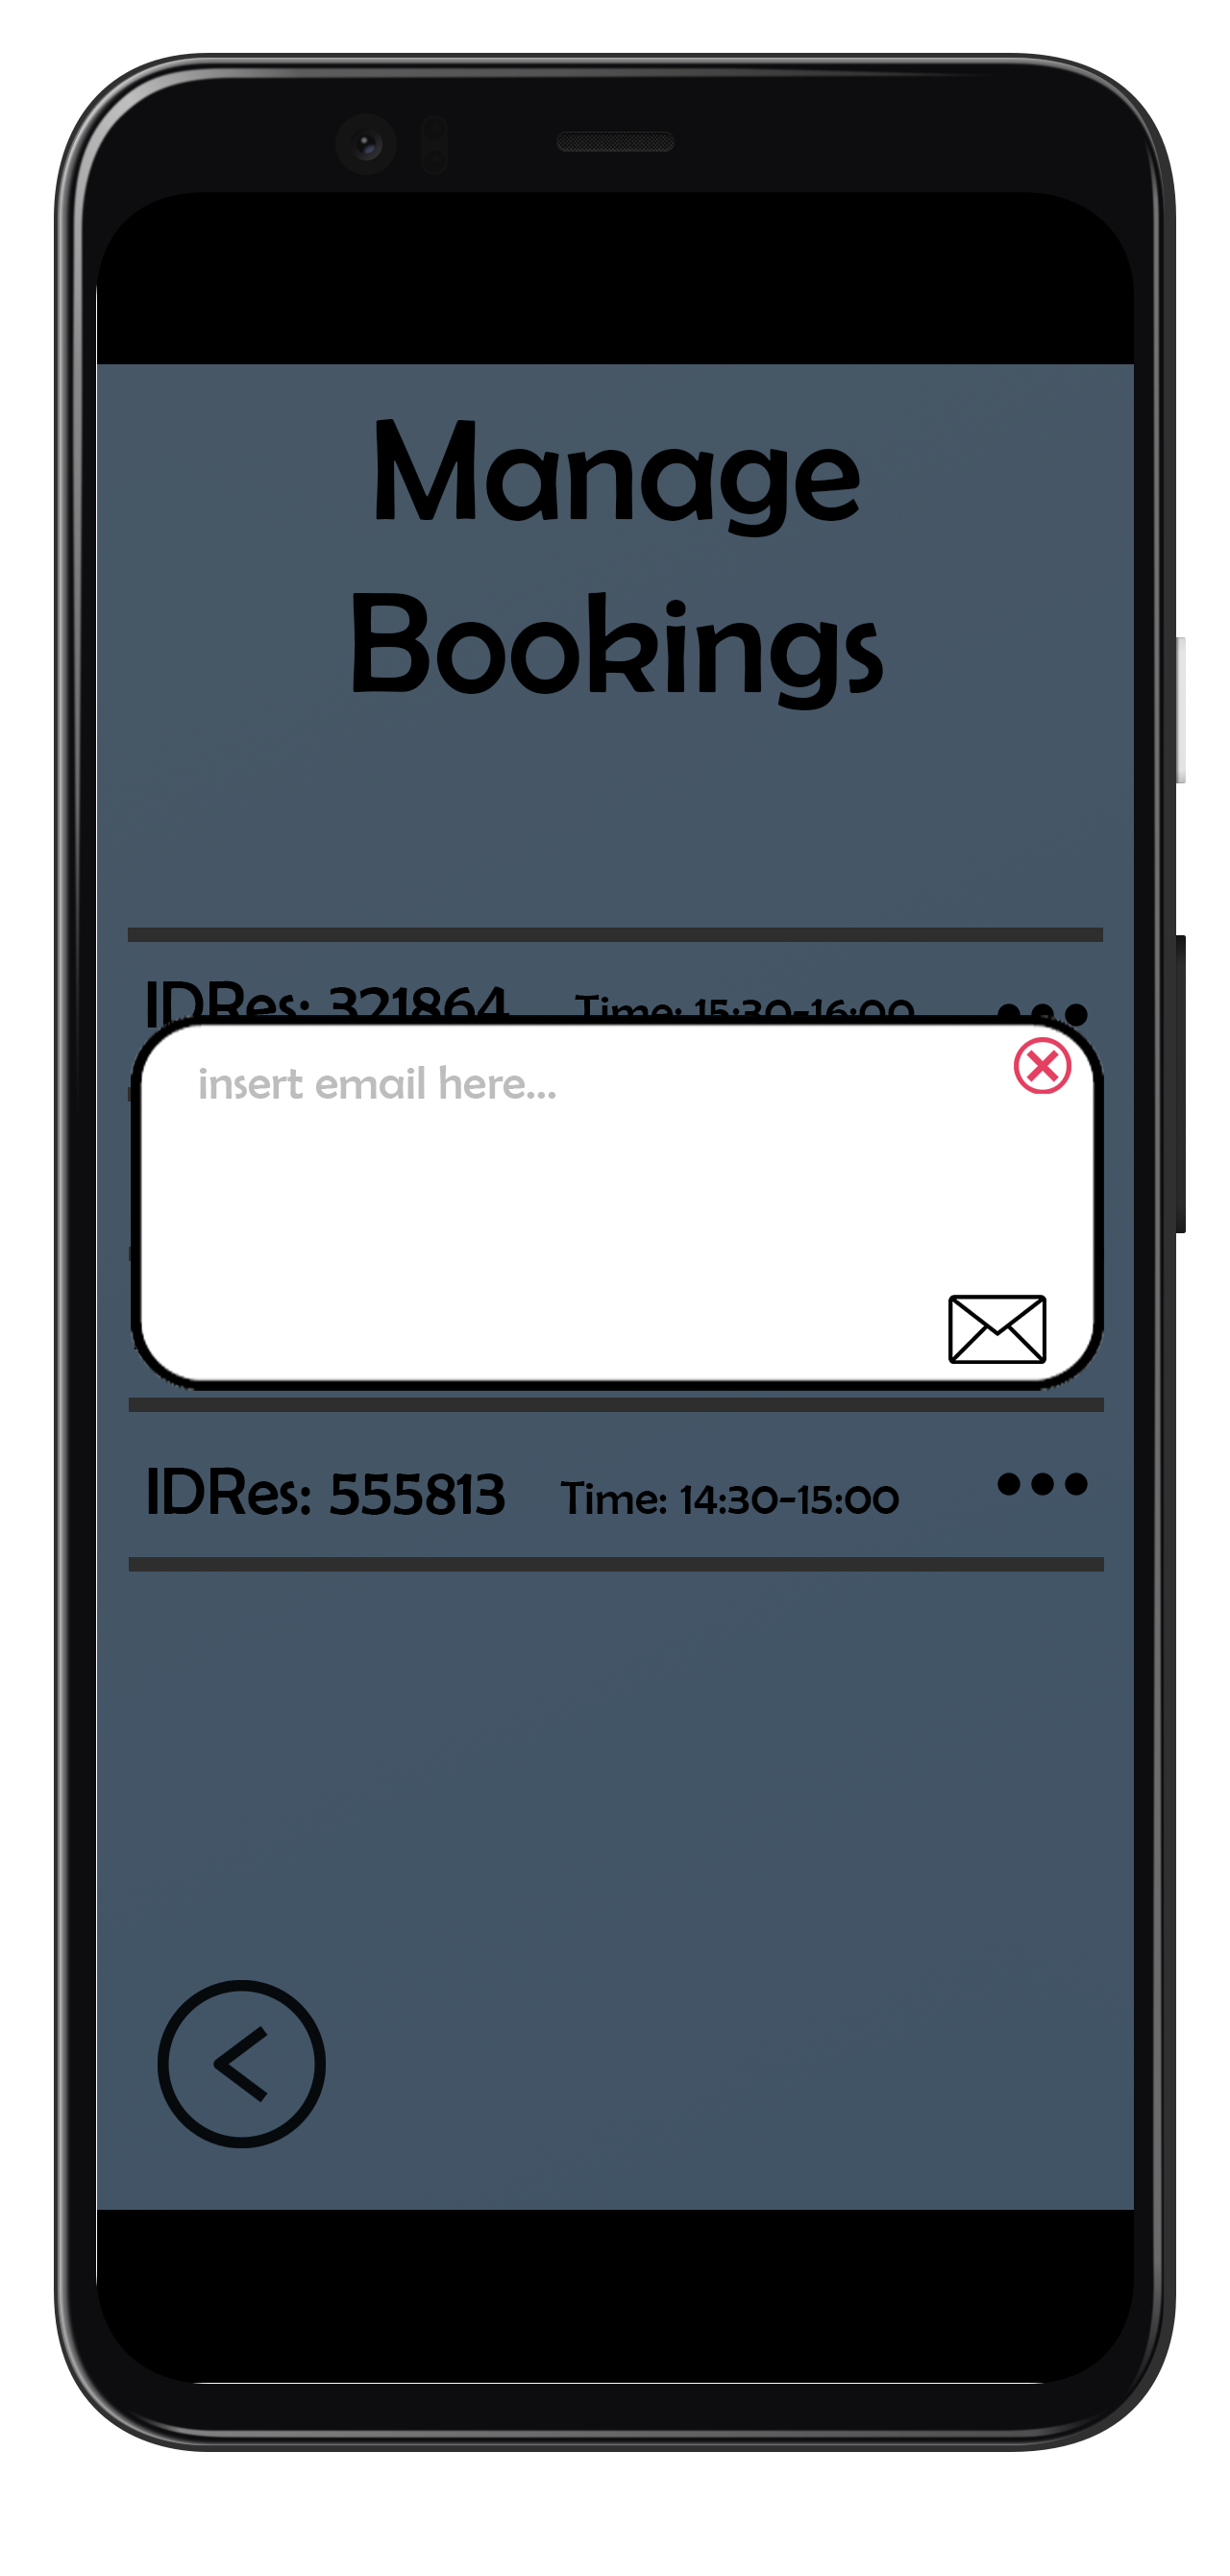
\includegraphics[scale=0.45]{../Mockups/MBpopup2}\\
				\end{adjustwidth}
				\caption{\emph{Contact client}}
			\end{figure}
		
			\begin{figure}[H]
				\begin{adjustwidth} {-4cm}{}
					\centering
					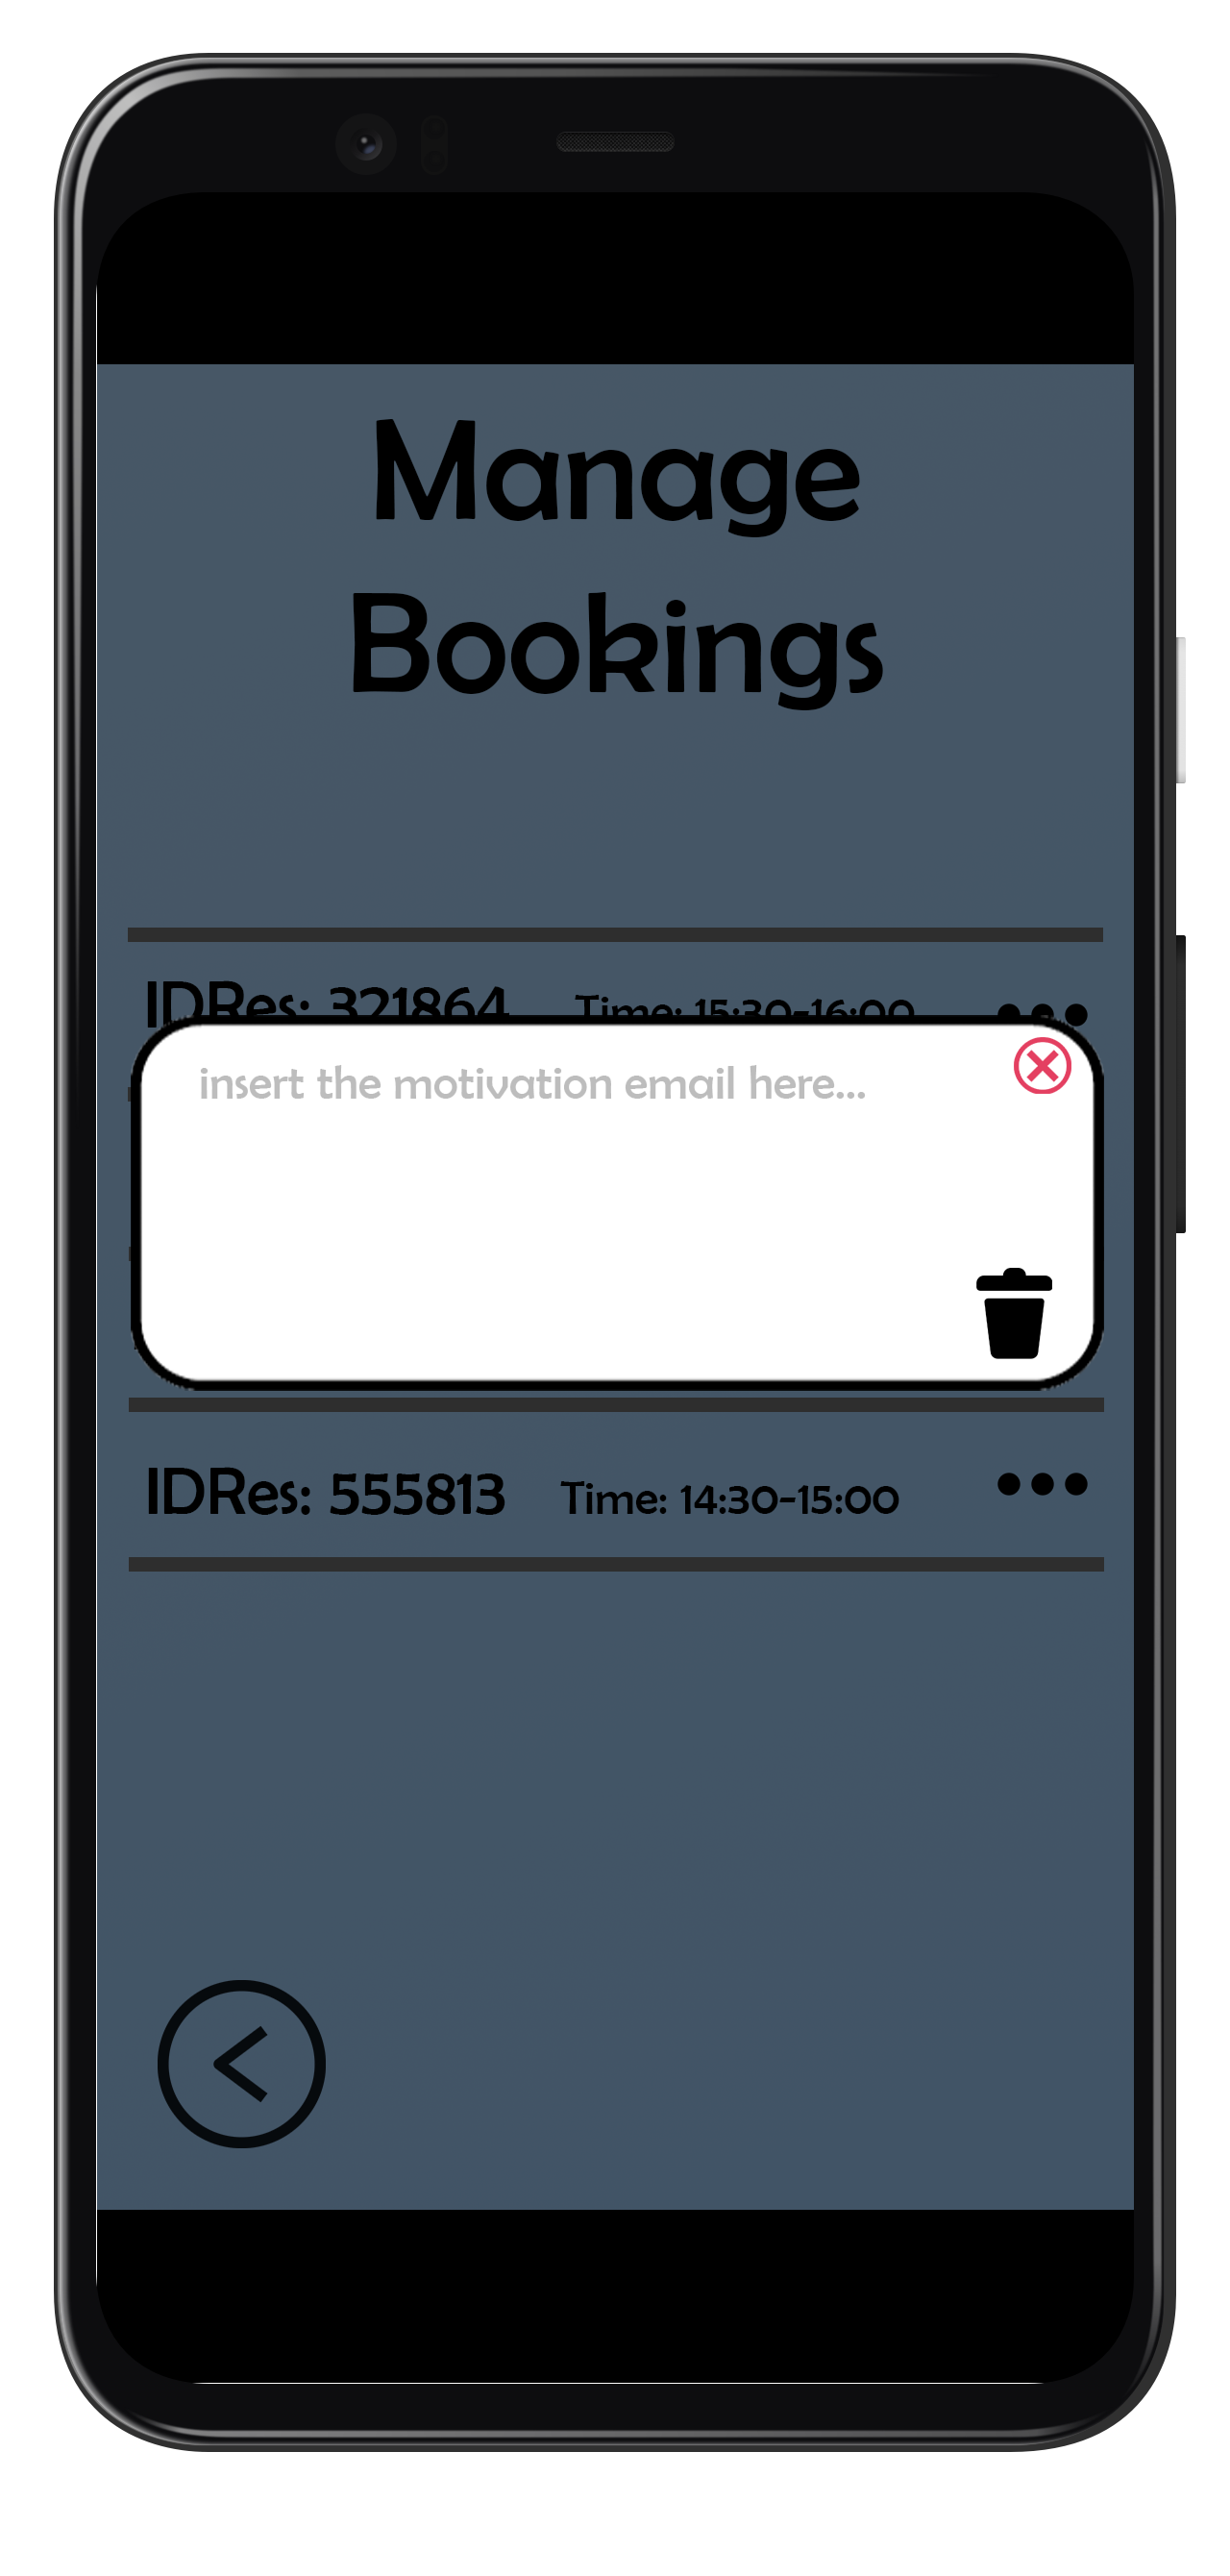
\includegraphics[scale=0.45]{../Mockups/MBpopup3}\\
				\end{adjustwidth}
				\caption{\emph{Cancel booking}}
			\end{figure}
		
		\subsubsection{Monitor store}
		
		Clicking on "Monitor store" will bring us to Figure ???, in which we can see all the statistics related to our store
		
		\begin{figure}[H]
			\begin{adjustwidth} {-4cm}{}
				\centering
				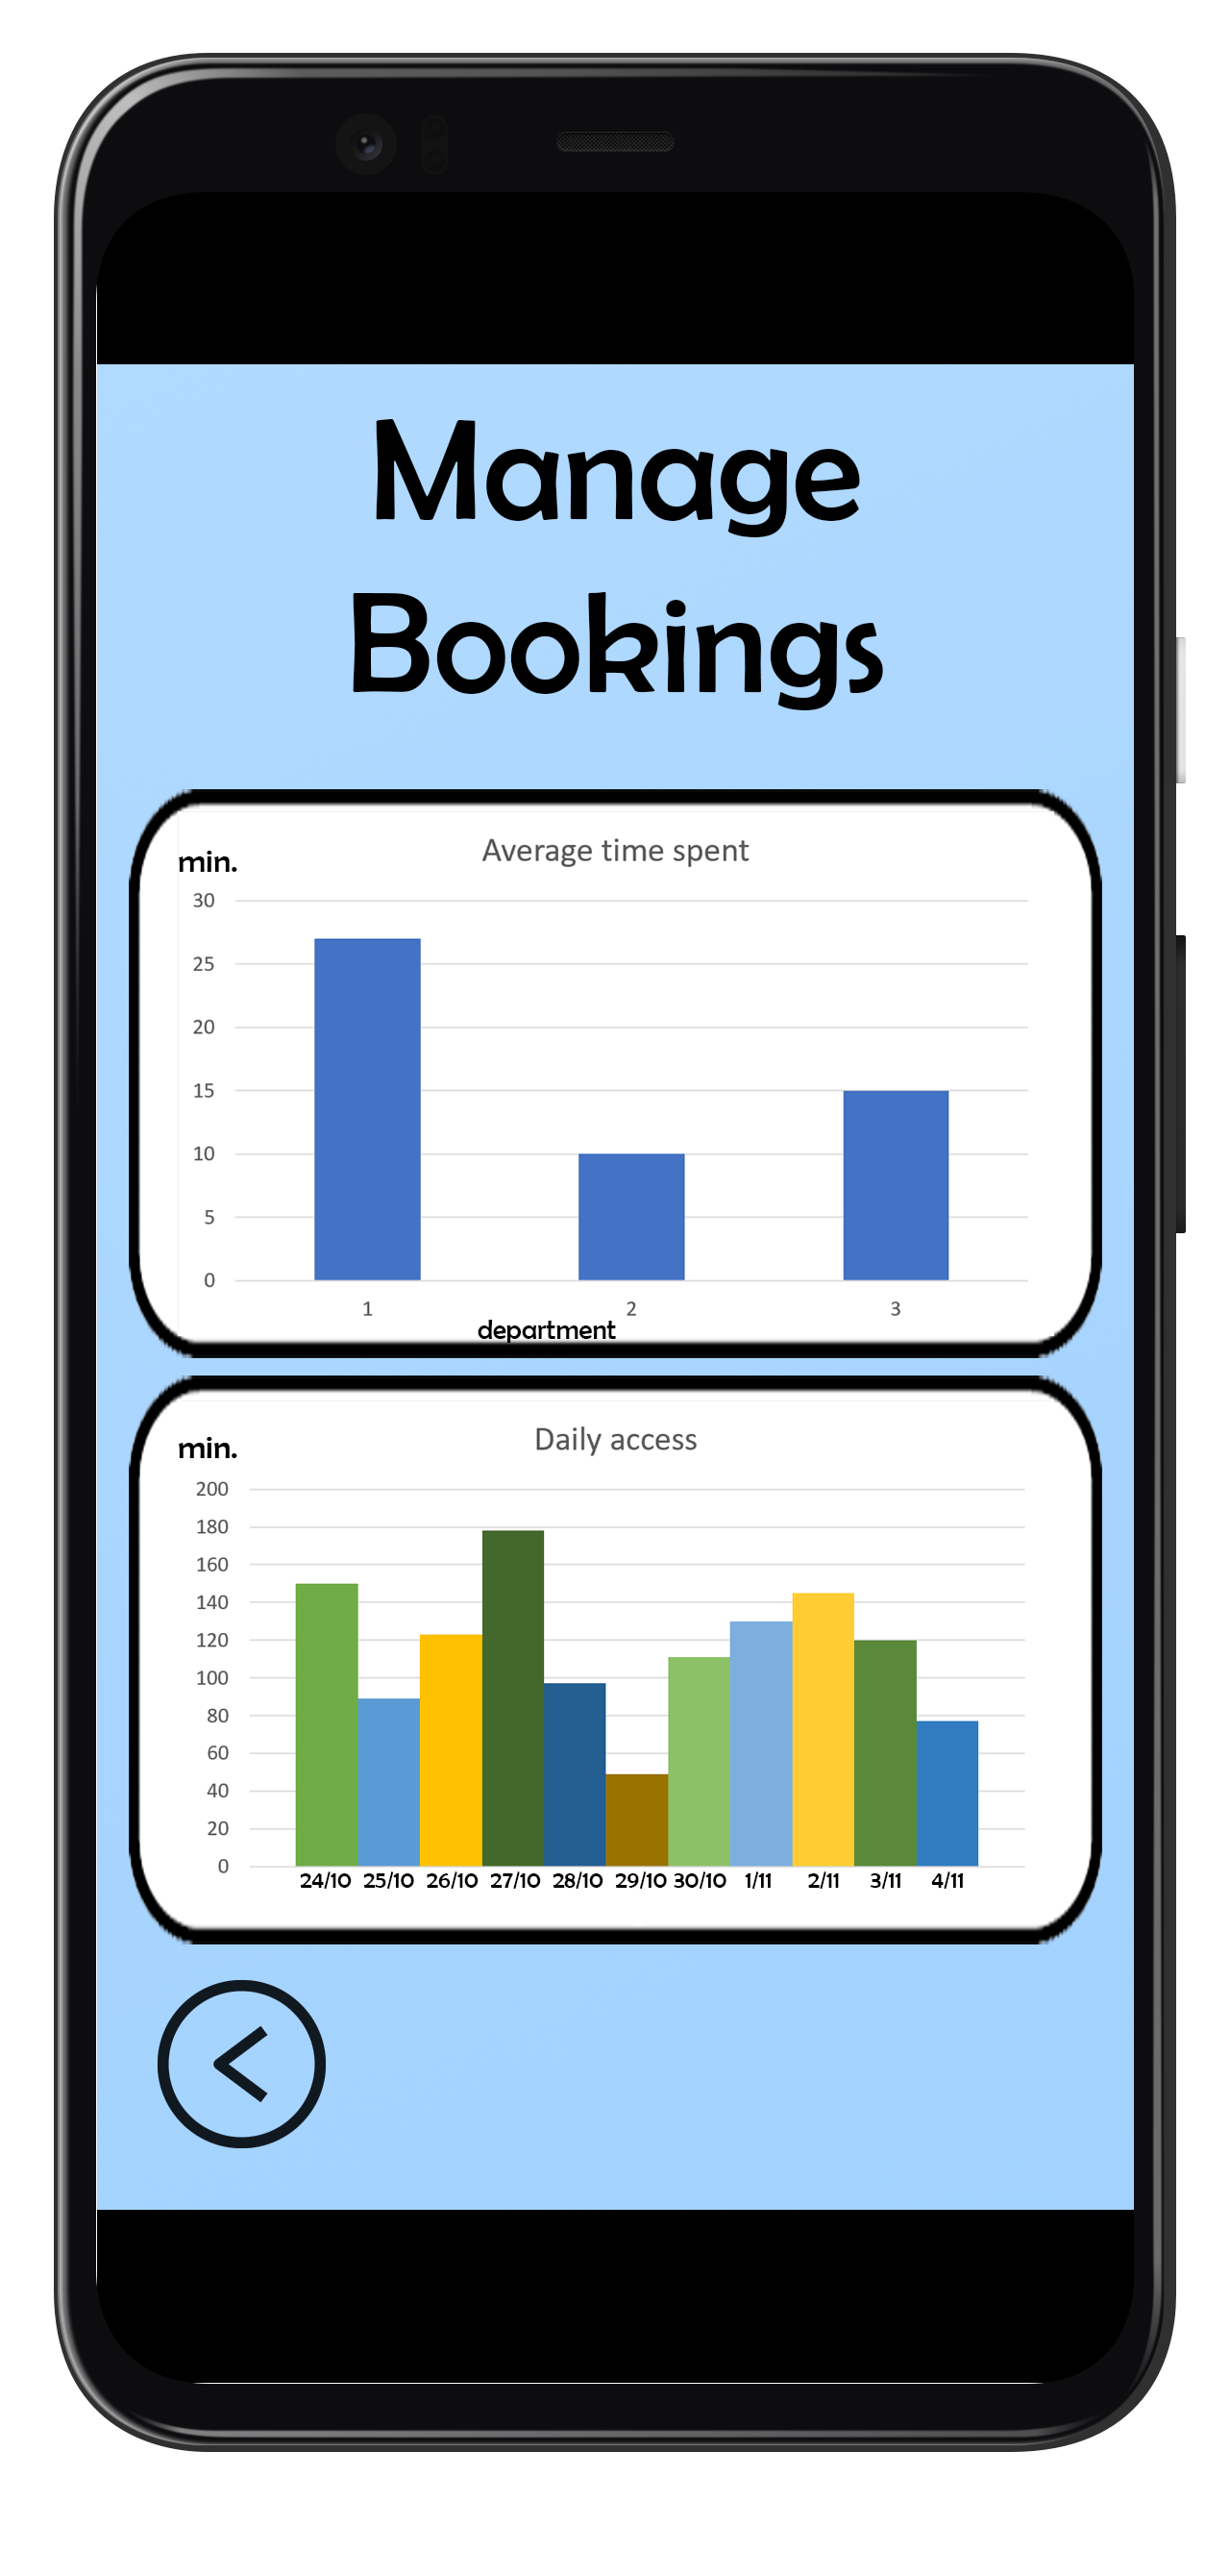
\includegraphics[scale=0.45]{../Mockups/Statistics.png}\\
			\end{adjustwidth}
			\caption{\emph{Monitor store}}
		\end{figure}
		
		\subsubsection{Modify parameters}
		
		Clicking on "Modify parameters" will bring us to Figure ???, in which we can:
		- see our daily settings;
		- change our general settings (store name, password, max wait time, max simultaneous booking per week and departments settings);
		- change our daily settings (closing day, opening and closure hours);
		- save changes or go back without saving.
		
		\begin{figure}[H]
			\begin{adjustwidth} {-4cm}{}
				\centering
				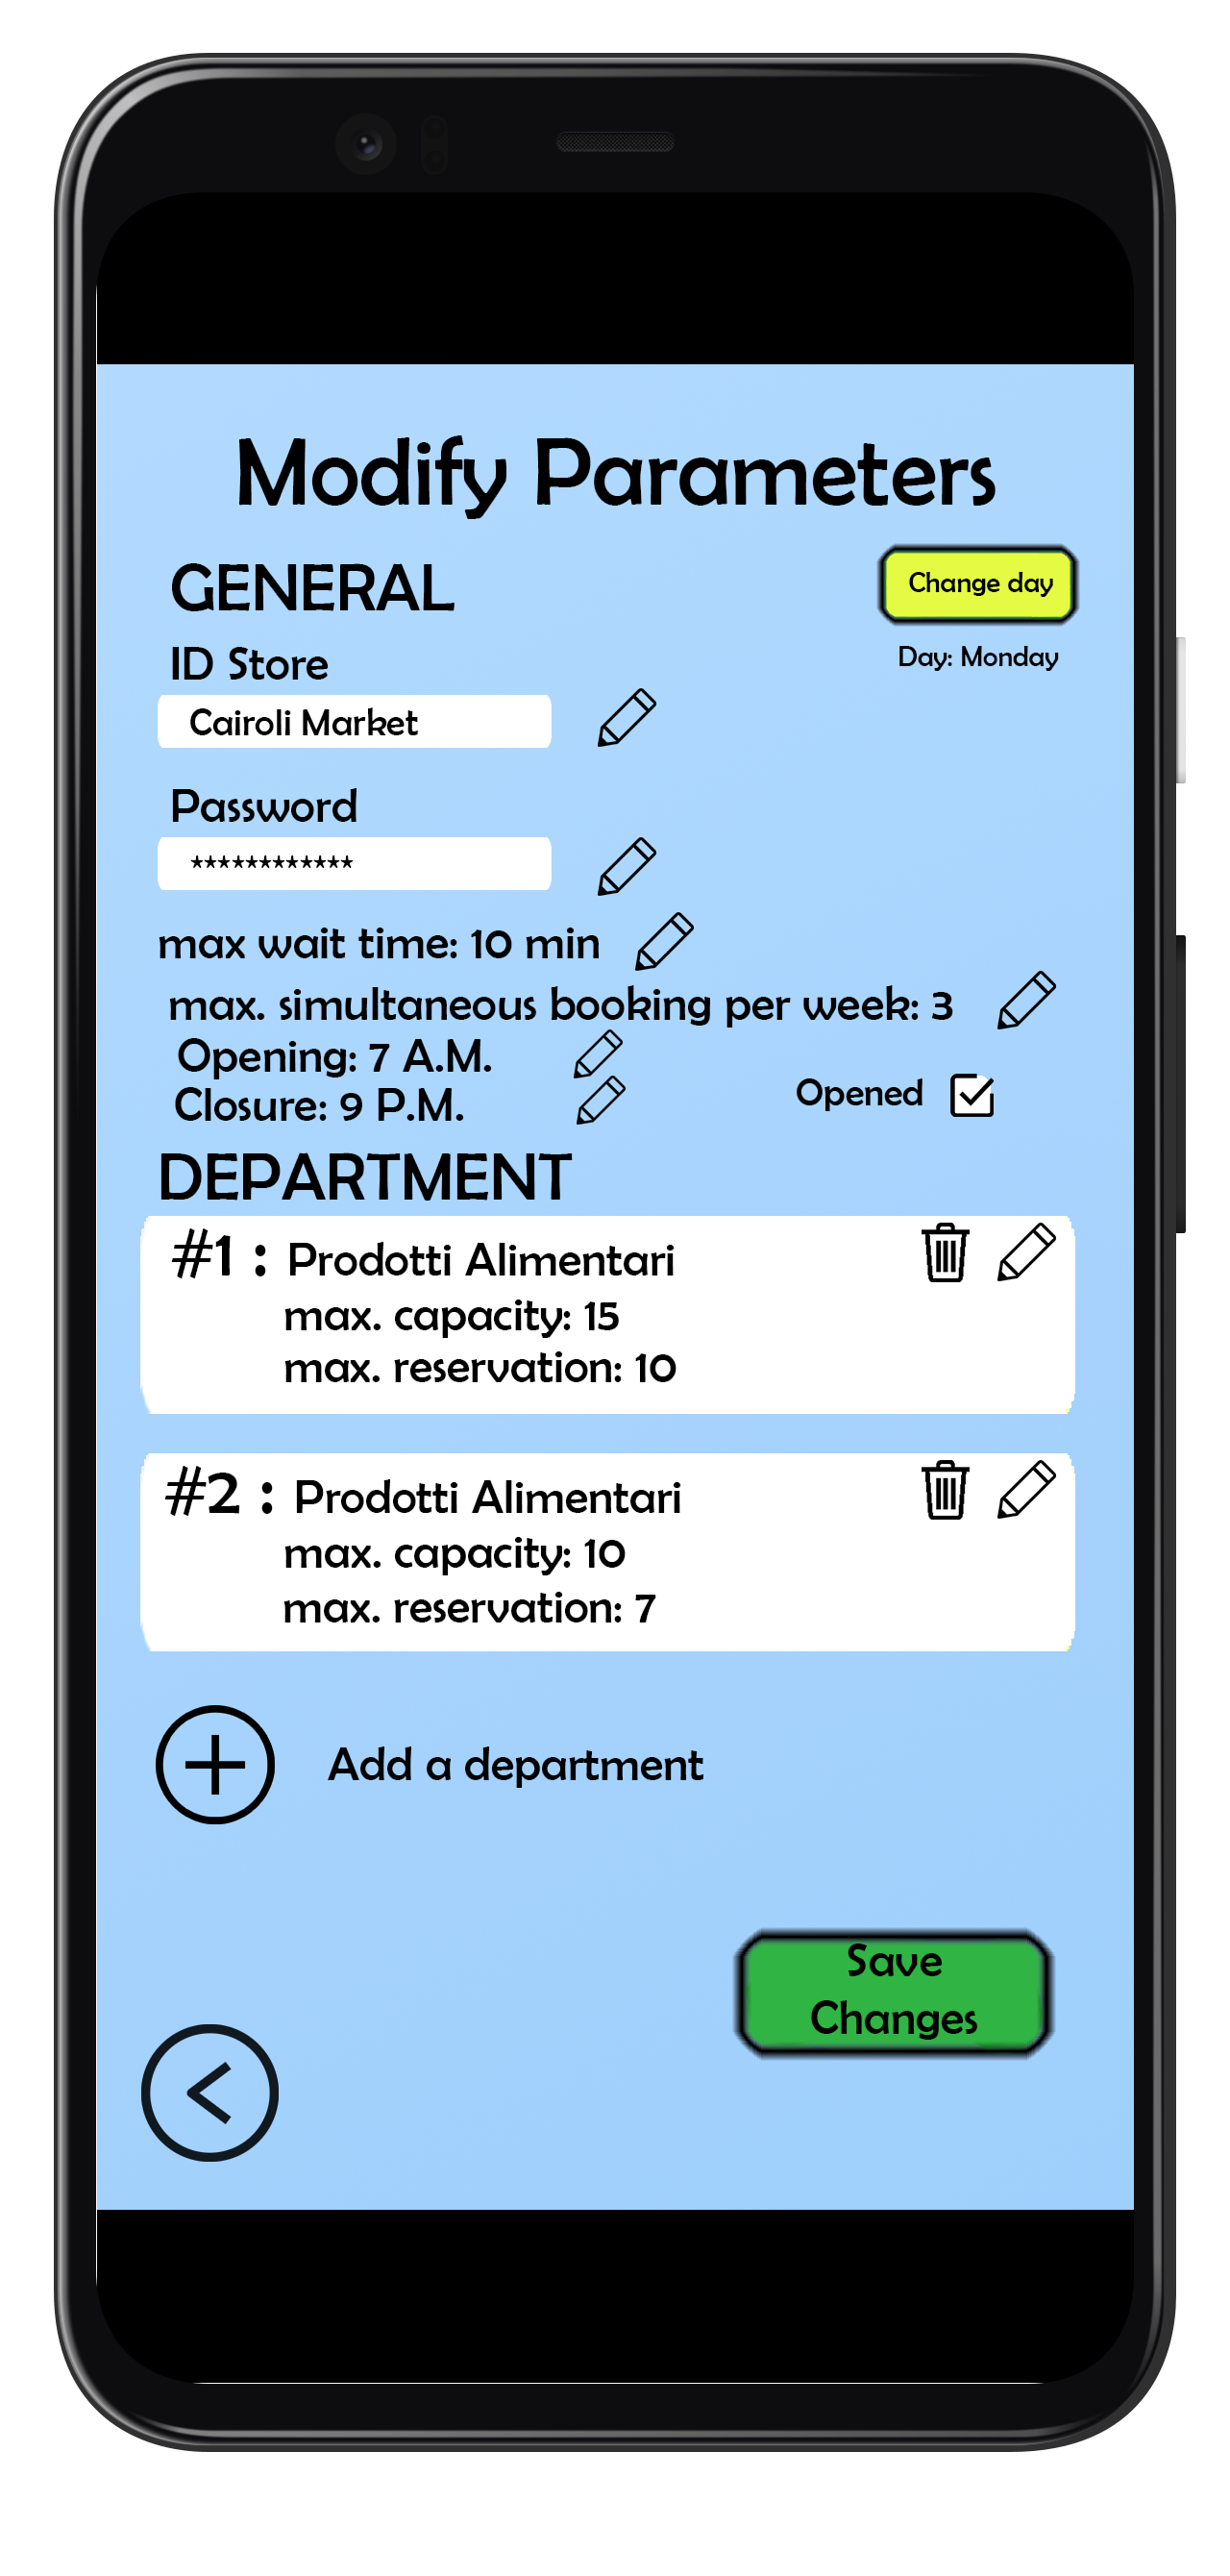
\includegraphics[scale=0.45]{../Mockups/ModifyParameters.png}\\
			\end{adjustwidth}
			\caption{\emph{Modify parameters}}
		\end{figure}
		
		
	




\section{Requirements Tracebility}

\section{Implementation, Integration and Test Plan}

\section{Effort Spent}

\section{References}
\end{document}.